\documentclass[12pt,english]{article}
%DIF LATEXDIFF DIFFERENCE FILE
%DIF DEL old versions for comparison/full_article_june2016.tex   Mon Feb 20 17:16:11 2017
%DIF ADD full_article.tex                                        Mon Feb 20 16:57:54 2017
\usepackage[affil-it]{authblk}
\usepackage{graphicx}
\usepackage[space]{grffile}
\usepackage{latexsym}
\usepackage{textcomp}
\usepackage{longtable}
\usepackage[flushleft]{threeparttable} 
\usepackage{multirow,booktabs}
\usepackage{amsfonts,amsmath,amssymb}
\usepackage{url}
%DIF 12c12
%DIF < %\usepackage[utf8]{inputenc}
%DIF -------
\usepackage[utf8]{inputenc} %DIF > 
%DIF -------
\usepackage{hyperref}
\hypersetup{colorlinks=false,pdfborder={0 0 0}}
%\usepackage{latexml}
\newcommand{\truncateit}[1]{\truncate{0.8\textwidth}{#1}}
\newcommand{\scititle}[1]{\title[\truncateit{#1}]{#1}}
%DIF 18c18
%DIF < \usepackage{lmodern}
%DIF -------
%\usepackage{lmodern} %DIF > 
%DIF -------
\usepackage[T1]{fontenc}
%DIF 20c20-21
%DIF < \usepackage[latin9]{inputenc}
%DIF -------
%\usepackage[latin9]{inputenc} %DIF > 
%\pagenumbering{gobble} %DIF > 
%DIF -------

\providecommand{\tabularnewline}{\\}
\usepackage[nolist]{acronym}
\newacro{BMI} {body mass index}  
\newacro{LMICs} {low- and middle-income countries}  
\newacro{LMIC} {low- and middle-income country}  
\newacro{MICs} {middle-income countries} 
\acrodefplural{HIC}[HICs]{high-income countries}
\newacro{MIC} {middle-income country}  
\newacro{HIC} {high-income country}  
 \newacro{FE} {fixed effects}  
\newacro{HbA1c} {glycated hemoglobin}  
\newacro{IDF} {International Diabetes Federation}  
\newacro{IV} {instrumental variable}  
\newacro{LPM} {linear probability model}  
\newacro{MxFLS} {Mexican Family Life Survey}  
\newacro{OLS} {ordinary least squares}  
\newacro{RE} {random effects}  
\newacro{US} {United States}
\newacro{WHO} {World Health Organization} 
\newacro{USA} {United States of America}   
%DIF 42d43
%DIF < \newacro{p.p.} {percentage points} 
%DIF -------
\usepackage{longtable}
\usepackage{booktabs}
\usepackage{multirow}
\usepackage{graphicx}
\usepackage[Export]{adjustbox}
%\newcommand{\sym}[1]{\ensuremath{^{#1}}} % for symbols in Table
%landscape pages
\usepackage{pdflscape}
\newcommand{\comment}[1]{}  %allows multiline comments
%DIF 52c52
%DIF < %\usepackage[english]{babel}% Recommended
%DIF -------
\usepackage[english]{babel}% Recommended %DIF > 
%DIF -------
%\usepackage{csquotes}
\usepackage[
maxcitenames=2, 
style=authoryear-comp,
firstinits=true,
maxbibnames=99,
backend=biber,
uniquename=false,
%DIF 61c61
%DIF < url=true,
%DIF -------
url=false, %DIF > 
%DIF -------
isbn=false]{biblatex}
\DeclareNameAlias{sortname}{last-first}
\DeclareFieldFormat{pages}{#1}%
\renewcommand*{\nameyeardelim}{\addcomma\space} %adds comma between name and years in citations

\renewbibmacro{in:}{}
\renewbibmacro*{volume+number+eid}{%
  \printfield{volume}%
  \setunit*{\adddot}% DELETED
  \setunit*{\addnbspace}% NEW (optional); there's also \addnbthinspace
 \printfield{number}%
 \setunit{\addcomma\space}%
 \printfield{eid}}
\DeclareFieldFormat[article]{number}{\mkbibparens{#1}}
\DeclareLanguageMapping{english}{english-apa}  %needed for APA style
\AtEveryBibitem{
  \clearfield{labelmonth}
}

%DIF 81c81-90
%DIF < \addbibresource{/home/till/Dokumente/BibTex/Second_Mexico_paper-Article.bib}
%DIF -------
\DeclareCiteCommand{\fullcite} %DIF > 
  {\usebibmacro{prenote}} %DIF > 
  {\usedriver %DIF > 
     {\defcounter{minnames}{6}% %DIF > 
      \defcounter{maxnames}{6}} %DIF > 
     {\thefield{entrytype}}.} %DIF > 
  {\multicitedelim} %DIF > 
  {\usebibmacro{postnote}} %DIF > 
%\addbibresource{/home/till/Dokumente/BibTex/Second_Mexico_paper-Article.bib} %DIF > 
\addbibresource{/home/till/Dokumente/BibTex/Thesis.bib} %DIF > 
%DIF -------
%\usepackage[authoryear]{natbib}


% paper margins
\usepackage{geometry}
\geometry{
letterpaper,
left=25mm,
right=30mm,
top=20mm,
bottom=30mm,
}   
%limiting tables to only float within section
%DIF 95c104
%DIF < \usepackage[section]{placeins}
%DIF -------
\usepackage{placeins} %DIF > 
%DIF -------
  
%use for commands only working with pdf
  
% formatation

\usepackage{listings}
\lstset{ %
  backgroundcolor=\color{white},   % choose the background color
  basicstyle=\footnotesize,        % size of fonts used for the code
  breaklines=true,                 % automatic line breaking only at whitespace
  captionpos=b,                    % sets the caption-position to bottom
  commentstyle=\color{OliveGreen},    % comment style
  keywordstyle=\color{BlueViolet},       % keyword style
  stringstyle=\color{black},     % string literal style
  language=[AlLaTeX]TeX,             % Set your language (you can change the language for each code-block optionally)
  frame=lrtb, %
  xleftmargin=\fboxsep, %
  xrightmargin=-\fboxsep, %
  moretexcs={lstset,color,colorlet, cellcolor, newcolumntype, columncolor, rowcolor, multirow, xspace, LaTeX, TeX},
}

	% *****************************************************************
	% siunitx
	% *****************************************************************
	\usepackage{siunitx} % centering in tables
		\sisetup{
			detect-mode,
			tight-spacing		= true,
			group-digits		= false ,
			input-signs		= ,
			input-symbols		= ( ) [ ] - + *,
			input-open-uncertainty	= ,
			input-close-uncertainty	= ,
			table-align-text-post	= false
	        }
\usepackage[firstpage]{draftwatermark}	         %DIF > 
%DIF PREAMBLE EXTENSION ADDED BY LATEXDIFF
%DIF UNDERLINE PREAMBLE %DIF PREAMBLE
\RequirePackage[normalem]{ulem} %DIF PREAMBLE
\RequirePackage{color}\definecolor{RED}{rgb}{1,0,0}\definecolor{BLUE}{rgb}{0,0,1} %DIF PREAMBLE
\providecommand{\DIFaddtex}[1]{{\protect\color{blue}\uwave{#1}}} %DIF PREAMBLE
\providecommand{\DIFdeltex}[1]{{\protect\color{red}\sout{#1}}}                      %DIF PREAMBLE
%DIF SAFE PREAMBLE %DIF PREAMBLE
\providecommand{\DIFaddbegin}{} %DIF PREAMBLE
\providecommand{\DIFaddend}{} %DIF PREAMBLE
\providecommand{\DIFdelbegin}{} %DIF PREAMBLE
\providecommand{\DIFdelend}{} %DIF PREAMBLE
%DIF FLOATSAFE PREAMBLE %DIF PREAMBLE
\providecommand{\DIFaddFL}[1]{\DIFadd{#1}} %DIF PREAMBLE
\providecommand{\DIFdelFL}[1]{\DIFdel{#1}} %DIF PREAMBLE
\providecommand{\DIFaddbeginFL}{} %DIF PREAMBLE
\providecommand{\DIFaddendFL}{} %DIF PREAMBLE
\providecommand{\DIFdelbeginFL}{} %DIF PREAMBLE
\providecommand{\DIFdelendFL}{} %DIF PREAMBLE
%DIF END PREAMBLE EXTENSION ADDED BY LATEXDIFF
%DIF PREAMBLE EXTENSION ADDED BY LATEXDIFF
%DIF HYPERREF PREAMBLE %DIF PREAMBLE
\providecommand{\DIFadd}[1]{\texorpdfstring{\DIFaddtex{#1}}{#1}} %DIF PREAMBLE
\providecommand{\DIFdel}[1]{\texorpdfstring{\DIFdeltex{#1}}{}} %DIF PREAMBLE
%DIF END PREAMBLE EXTENSION ADDED BY LATEXDIFF

\begin{document}
\title{The impact of diabetes on labor market outcomes in Mexico: a panel data and biomarker analysis\DIFaddbegin \thanks{Till Seuring is a post-doctoral researcher at the Leibniz Institute for Prevention Research and Epidemiology - BIPS and his email is seuring@leibniz-bips.de,  Pieter Serneels is Associate Professor at University of East Anglia and can be contacted at p.serneels@uea.ac.uk, Marc Suhrcke is Professor at the University of York and his email is marc.suhrcke@york.ac.uk.}\DIFaddend }

\DIFdelbegin %DIFDELCMD < \author[a]{%%%
\DIFdelend \DIFaddbegin \author[1,2]{\DIFaddend Till Seuring%
	\thanks{Corresponding author}}
\DIFdelbegin %DIFDELCMD < \author[b]{%%%
\DIFdelend \DIFaddbegin \author[2]{\DIFaddend Pieter Serneels}
\DIFdelbegin %DIFDELCMD < \author[c]{%%%
\DIFdelend \DIFaddbegin \author[3]{\DIFaddend Marc Suhrcke}

\DIFdelbegin %DIFDELCMD < \affil[a]{Norwich Medical School, University of East Anglia, Norwich Research Park, Norwich, Norfolk, NR47TJ, UK, t.seuring@uea.ac.uk}
%DIFDELCMD < \affil[b]{School of International Development, University of East Anglia, Norwich Research Park, Norwich, Norfolk, NR47TJ, UK, p.serneels@uea.ac.uk}
%DIFDELCMD < \affil[c]{Centre for Health Economics, University of York, Heslington, York, YO105DD, UK, marc.suhrcke@york.ac.uk}
%DIFDELCMD < \date{}
%DIFDELCMD < %%%
\DIFdelend \DIFaddbegin \affil[1]{Leibniz Institute for Prevention Research and Epidemiology - BIPS}
\affil[2]{University of East Anglia}
\affil[3]{University of York}
\DIFaddend 





\maketitle 
\DIFdelbegin %DIFDELCMD < 

%DIFDELCMD < %%%
\DIFdelend \begin{abstract}
\DIFdelbegin \DIFdel{There is limited evidence on the labor market impact of diabetes, and existing evidence tends to be weakly identified}\DIFdelend \DIFaddbegin \DIFadd{Diabetes has become one of the most common chronic diseases in middle- and high-income countries. Yet, our understanding of its economic consequences remains limited}\DIFaddend . Making use of \DIFdelbegin \DIFdel{Mexican panel data to estimate individual fixed effects models}\DIFdelend \DIFaddbegin \DIFadd{rich panel data for Mexico, where diabetes is the number one cause of death}\DIFaddend , we find evidence for adverse effects of self-reported diabetes on \DIFdelbegin \DIFdel{employment probabilities}\DIFdelend \DIFaddbegin \DIFadd{the probability of being employed}\DIFaddend , but not on wages or hours worked\DIFdelbegin \DIFdel{. Complementary biomarker information for a cross section indicates that a large diabetes population is unaware of the disease.  When accounting for this, the negative relationship }\DIFdelend \DIFaddbegin \DIFadd{, using fixed effects estimation. Self-reported diabetes reduces the probability of employment with 5 percentage points for men and close to 6 percentage points for women.  Considering different types of work, the relationship between self-reported diabetes, and wages and hours worked remains weak, but the results also suggest occupational selection with women with self-reported diabetes less likely to work in agriculture.  A dynamic analysis finds that the employment probability falls gradually over the years after having been diagnosed with this chronic condition.  Using unique biomarker data for a large subsample, we find that two thirds of those tested positive do not self-report diabetes, while 19}\% \DIFadd{of those who self-report have levels below the clinical threshold.  We contrast the impact }\DIFaddend of self-reported \DIFdelbegin \DIFdel{diabetes with employment remains, but does not extend to those unaware of their diabetes.  Further analysis suggests that this difference stems from worse general health among the self-reports rather than more }\DIFdelend \DIFaddbegin \DIFadd{and tested diabetes, and find that it is similar for women but not for men.  Combined results suggest lower employment for those self-reporting, especially for men, while there is no employment effect for undiagnosed men or women, who tested positive but did not self-report.  This lack of employment effect for undiagnosed men seems to stem from better general health rather than less }\DIFaddend severe diabetes. \DIFaddbegin \DIFadd{The results highlight both the importance of the economic impact of diabetes, and the need to take into account (especially female) undiagnosed patients.
}\DIFaddend \end{abstract}



\DIFdelbegin %DIFDELCMD < {\bf %%%
\DIFdel{Keywords:}%DIFDELCMD < } %%%
\DIFdel{diabetes; labor market; Mexico; biomarker; panel data
}%DIFDELCMD < 

%DIFDELCMD < %%%
\DIFdelend \section{\DIFdelbegin %DIFDELCMD < \label{sec:Introduction}%%%
\DIFdelend \DIFaddbegin \label{sec:Introduction4}\DIFaddend Introduction }

Diabetes, and particularly its most common variant, type 2 diabetes, has increased worldwide and is expected to continue to rise over the next decades \parencite{Risk2016}. \DIFdelbegin \DIFdel{It }\DIFdelend \DIFaddbegin \DIFadd{The condition }\DIFaddend has become a problem for \DIFdelbegin %DIFDELCMD < \ac{MICs} %%%
\DIFdel{and }%DIFDELCMD < \acp{HIC} %%%
\DIFdelend \DIFaddbegin \DIFadd{middle-income countries and high-income countries }\DIFaddend alike, with over two-thirds of people with diabetes living in the developing world \parencite{InternationalDiabetesFederation2013}. Mexicans and Mexican-Americans appear to be particularly affected by diabetes, also in comparison to other Latino populations living in the \DIFdelbegin %DIFDELCMD < \ac{USA} %%%
\DIFdelend \DIFaddbegin \DIFadd{USA }\DIFaddend \parencite{Schneiderman2014}. In Mexico itself, diabetes prevalence has been estimated to have grown from 6.7\% in 1994 to 14.4\% in 2006, including both diagnosed and undiagnosed cases \parencite{Barquera2013}, and is expected to increase further over the next decades \parencite{Meza2015}. Already now, diabetes is the number one cause of death in Mexico \parencite{Barquera2013}. 

The observed trend has been attributed to a deterioration in diet and a reduction in physical activity \parencite{Barquera2008b,Basu2013}, while genetic predisposition among Mexicans with pre-hispanic ancestry may also \DIFdelbegin \DIFdel{have played }\DIFdelend \DIFaddbegin \DIFadd{play }\DIFaddend a role \parencite{Williams2013}. Recent evidence indicates that the onset of diabetes has been occurring at an ever earlier age in Mexico \parencite{Villalpando2010}. With treatment as ineffective as it currently \DIFdelbegin \DIFdel{is ---only }\DIFdelend \DIFaddbegin \DIFadd{is---only }\DIFaddend a minority achieves adequate blood glucose control \parencite{Barquera2013}\DIFdelbegin \DIFdel{--- the earlier onset }\DIFdelend \DIFaddbegin \DIFadd{---the earlier start }\DIFaddend will increase the likelihood of complications during the productive lifespan. 

Diabetes is a term used to describe various conditions characterized by high blood glucose values, with the predominant disease being type 2 diabetes accounting for about 90\DIFdelbegin \DIFdel{percent }\DIFdelend \DIFaddbegin \% \DIFaddend of all diabetes cases \parencite{Sicree2009}. The elevated
blood glucose levels that are a result of the body's inability to use insulin properly to maintain blood glucose at normal levels, can entail a range of adverse health effects for the individual concerned. However, via effective self-management of the disease much if not all of the complications can be avoided \parencite{Lim2011, Gregg2012}. In the absence of \DIFdelbegin \DIFdel{effective self-management ---or }\DIFdelend \DIFaddbegin \DIFadd{this management---or }\DIFaddend in the case of inadequate \DIFdelbegin \DIFdel{treatment--- diabetes }\DIFdelend \DIFaddbegin \DIFadd{treatment---diabetes }\DIFaddend has been documented to lead to conditions such as heart disease and stroke, blindness, kidney problems, and nerve problems which together with impaired wound healing can lead to the loss of limbs \parencite{Reynoso-Noveron2011}. These conditions can be seriously debilitating and may therefore reduce an individual's economic activity, including its productivity and labor market participation.

The effect of diabetes on labor \DIFdelbegin \DIFdel{market }\DIFdelend outcomes has been studied predominantly in \DIFdelbegin %DIFDELCMD < \acp{HIC} %%%
\DIFdel{---with the exception of a study on Mexico }%DIFDELCMD < \autocite{Seuring2015} %%%
\DIFdel{and one on China }%DIFDELCMD < \parencite{Liu2014} %%%
\DIFdel{each. In the }%DIFDELCMD < \ac{HIC} %%%
\DIFdel{studies }\DIFdelend \DIFaddbegin \DIFadd{high-income countries where }\DIFaddend diabetes has been found to be associated with reductions in employment probabilities as well as wages and labor supply \DIFdelbegin %DIFDELCMD < \parencite{Brown2005,Brown2014,BrownIII2011,Minor2010,Minor2013,Minor2015,Latif2009,Seuring2015a}%%%
\DIFdel{.}\DIFdelend \DIFaddbegin \parencite{Brown2005,Brown2014,BrownIII2011,Minor2011,Minor2013,Minor2015,Latif2009,Seuring2015a}\DIFadd{.}\footnote{\DIFadd{We know of only two studies for middle income countries, one for Mexico }\parencite{Seuring2015} \DIFadd{and one for China }\parencite{Liu2014}\DIFadd{, which are discussed later in more detail.}}
\DIFaddend 

While these studies have provided useful evidence \DIFdelbegin \DIFdel{on the potential labor market effects of diabetes}\DIFdelend , many of the complexities of the relationship \DIFdelbegin \DIFdel{have not been comprehensively addressed in any given study. First of all, unobserved }\DIFdelend \DIFaddbegin \DIFadd{between diabetes and labor outcomes remain have remained unaddressed. Unobserved }\DIFaddend heterogeneity presents a challenge \DIFdelbegin \DIFdel{to estimate }\DIFdelend \DIFaddbegin \DIFadd{when estimating }\DIFaddend the relationship between diabetes and labor outcomes. Especially time-invariant unobserved individual characteristics, \DIFdelbegin \DIFdel{e.g. health endowments ---often related to health during uteru, infant and child years, and to low household income or adverse health shocks during these early years--- }\DIFdelend \DIFaddbegin \DIFadd{like health endowments , }\DIFaddend as well as risk preferences have been shown to adversely affect health in general and the propensity to develop type 2 diabetes more specifically \parencite{VanEwijk2011,Sotomayor2013,Li2010b}\DIFdelbegin \DIFdel{. These and other unobserved personal characteristics (e.g. ability) }\DIFdelend \DIFaddbegin \DIFadd{; they }\DIFaddend may also affect employment probabilities, wages or working \DIFdelbegin \DIFdel{hours }\DIFdelend \DIFaddbegin \DIFadd{hours---either }\DIFaddend directly through their effects on contemporaneous productivity \parencite{Currie2013} \DIFdelbegin \DIFdel{and }\DIFdelend \DIFaddbegin \DIFadd{or }\DIFaddend indirectly by limiting educational attainment and human capital accumulation \parencite{Ayyagari2011a}. Further, \DIFdelbegin \DIFdel{only focusing on the overall effect of a self-reported diabetes diagnosis does not reveal }\DIFdelend \DIFaddbegin \DIFadd{given the chronic nature of the condition, it would be of interest to better understand }\DIFaddend when potential labor market penalties appear, \DIFdelbegin \DIFdel{given the dynamic aspect of diabetes and the potential differences in its effects }\DIFdelend \DIFaddbegin \DIFadd{and how these effects change }\DIFaddend over time. 
\DIFdelbegin \DIFdel{Additionally, apart from its health impact diabetesmight also affect labor market outcomes through other channels. For instance, people }\DIFdelend \DIFaddbegin 

\DIFadd{Finally, given that most studies rely on self-reported diabetes data, it is of interest to contrast estimates obtained from this data with those yielded from clinical test data on diabetes. Especially in a middle income country setting, where large parts of the population remain undiagnosed, this can reveal hidden impacts, namely for those who are unaware of the disease. Diabetes may also have an effect in itself. People }\DIFaddend aware of their condition may\DIFaddbegin \DIFadd{, for instance, }\DIFaddend be less inclined to continue working if this interferes with their disease management\DIFdelbegin \DIFdel{or }\DIFdelend \DIFaddbegin \DIFadd{, they may }\DIFaddend be suffering from psychological \DIFdelbegin \DIFdel{consequences (depression, anxiety) }\DIFdelend \DIFaddbegin \DIFadd{stress, depression, or anxiety, because }\DIFaddend of becoming aware of the disease; they may also use the diagnosis as a justification for decreasing their labor supply \DIFdelbegin \DIFdel{, leading to a potential justification bias in the estimated effect of diabetes }\DIFdelend \parencite{Kapteyn2009}. \DIFdelbegin \DIFdel{Importantly, for these reasons the }\DIFdelend \DIFaddbegin \DIFadd{As a consequence }\DIFaddend labor market effects may \DIFdelbegin \DIFdel{also }\DIFdelend be distinct for people with self-reported versus those unaware of their condition, potentially leading to biased estimates if the analysis is \DIFdelbegin \DIFdel{solely }\DIFdelend based on self-reports \DIFaddbegin \DIFadd{alone}\DIFaddend .

The objective of this study is to provide new evidence on the impact of diabetes on labor outcomes, \DIFdelbegin \DIFdel{while improving }\DIFdelend \DIFaddbegin \DIFadd{and improve }\DIFaddend upon previous work by paying close attention to the above challenges. We use three waves of panel data from \DIFdelbegin \DIFdel{Mexico }\DIFdelend \DIFaddbegin \DIFadd{the }\acf{MxFLS}\DIFadd{, }\DIFaddend covering the period 2002--2012\DIFdelbegin \DIFdel{, provided by the }%DIFDELCMD < \ac{MxFLS}%%%
\DIFdelend . The \ac{MxFLS} is particularly useful for the analysis of diabetes as it allows \DIFdelbegin \DIFdel{us to account }\DIFdelend \DIFaddbegin \DIFadd{accounting }\DIFaddend for the above complexities in \DIFdelbegin \DIFdel{a more refined way than has been the case so far}\DIFdelend \DIFaddbegin \DIFadd{more refined ways than existing studies}\DIFaddend . Using individual level \DIFdelbegin %DIFDELCMD < \ac{FE} %%%
\DIFdelend \DIFaddbegin \acf{FE} \DIFaddend analysis for the first time in this literature, we take account of time-invariant heterogeneity when assessing the impact of self-reported diabetes and \DIFdelbegin \DIFdel{self-reported diabetes }\DIFdelend \DIFaddbegin \DIFadd{its }\DIFaddend duration on labor \DIFdelbegin \DIFdel{market outcomes.}\DIFdelend \DIFaddbegin \DIFadd{outcomes.}\DIFaddend \footnote{\DIFdelbegin \DIFdel{We are not aware }\DIFdelend \DIFaddbegin \DIFadd{A recent review }\DIFaddend of \DIFdelbegin \DIFdel{any other evidence on }\DIFdelend the \DIFdelbegin \DIFdel{effect on wages }\DIFdelend \DIFaddbegin \DIFadd{economic cost of diabetes confirms the scarcity of evidence for low- }\DIFaddend and \DIFdelbegin \DIFdel{working hours in a }%DIFDELCMD < \ac{MIC}%%%
\DIFdelend \DIFaddbegin \DIFadd{middle-income countries }\parencite{Seuring2015a}\DIFaddend .}  \DIFdelbegin \DIFdel{Further, we add to the current literature in exploring the role of undiagnosed diabetes, using }\DIFdelend \DIFaddbegin \DIFadd{Using }\DIFaddend novel and rich biomarker data \DIFdelbegin \DIFdel{- an }\DIFdelend \DIFaddbegin \DIFadd{we also explore the role of undiagnosed diabetes---an }\DIFaddend issue of considerable importance in light of \DIFdelbegin \DIFdel{the large prevalence of undiagnosed diabetes }\DIFdelend \DIFaddbegin \DIFadd{its high prevalence }\DIFaddend (see \textcite{Beagley2014}) \DIFdelbegin \DIFdel{that }\DIFdelend \DIFaddbegin \DIFadd{and because it has }\DIFaddend remained unaccounted for in most earlier studies\DIFaddbegin \DIFadd{, }\DIFaddend which typically rely on self-reported information. Doing so sheds light on the issue of measurement error and the potentially differential effects of self-reported and undiagnosed diabetes.

Our results using self-reported diabetes suggest an economically important decrease in the employment probability of people aware of their disease. Wages and working hours, however, do not appear to be \DIFdelbegin \DIFdel{negatively associated }\DIFdelend \DIFaddbegin \DIFadd{lower for those }\DIFaddend with self-reported diabetes. \DIFdelbegin \DIFdel{We further find }\DIFdelend \DIFaddbegin \DIFadd{A dynamic analysis indicates }\DIFaddend that employment probabilities are reduced \DIFaddbegin \DIFadd{gradually }\DIFaddend with each additional year since diagnosis, with some evidence for an even larger effect per year after the initial 10 years.

The biomarker analysis indicates that \DIFdelbegin \DIFdel{self-reported }\DIFdelend \DIFaddbegin \DIFadd{clinically diagnosed }\DIFaddend diabetes entails a significant employment penalty \DIFdelbegin \DIFdel{, while biometrically measured diabetes does not . Overall, undiagnosed diabetes does not appear to affect any of }\DIFdelend \DIFaddbegin \DIFadd{for women but not for men. Assessing the effects of both clinical and self-reported diabetes at the same time provides an insight into }\DIFaddend the labor market \DIFdelbegin \DIFdel{outcomes examined here, suggesting that adverse effects mainly occur to those }\DIFdelend \DIFaddbegin \DIFadd{impact for those with undiagnosed diabetes---people who are tested positive but did not self-report. The results suggest that }\DIFaddend self-reporting \DIFdelbegin \DIFdel{a diagnosis. We argue that , nonetheless, the effects found for self-reported diabetes in this study are largely unbiased as long as inference is not extended to the unobserved undiagnosed population, and are economically important in light of the sheer size of the diagnosed population in Mexico.
}\DIFdelend \DIFaddbegin \DIFadd{in itself has a negative and significant effect for men, but the effect is not statistically significant for women, possibly  due to large standard errors. In contrast we find no evidence for an effect of undiagnosed diabetes. 
}\DIFaddend 


\DIFdelbegin \section{%DIFDELCMD < \label{sec:Labor  outcomes and diabetes literature} %%%
\DIFdel{Diabetes and labor outcomes -- existing evidence }}
%DIFAUXCMD
\addtocounter{section}{-1}%DIFAUXCMD
\DIFdelend \DIFaddbegin \section{\label{sec:labor  outcomes and diabetes literature}\DIFadd{Diabetes and labor outcomes---what do we know?}}
\DIFaddend 

\DIFdelbegin \DIFdel{Several }\DIFdelend \DIFaddbegin \DIFadd{A limited number of studies provides insights on the relationship between diabetes and labor outcomes.  Table 1 in appendix summarises the main findings of these studies, the characteristics of the sample and estimation method they use, and the approach to measure diabetes.  To the best of our knowledge only two studies exist for developing countries. \textcite{Liu2014} exploiting a natural experiment in China, find a significant reduction in income for those with a recent diagnosis of diabetes. A study for Mexico using cross-section data from 2005, finds a significant (p<0.01) reduction in employment probabilities for males by about 10 percentage points and for females by about 4.5 percentage points (p<0.1), using parental diabetes as an }\ac{IV} \parencite{Seuring2015}\DIFadd{.
}

\DIFadd{A small number of }\DIFaddend studies have investigated the effects of diabetes on labor \DIFdelbegin \DIFdel{market outcomes . 
}%DIFDELCMD < 

%DIFDELCMD < %%%
\DIFdel{For the }%DIFDELCMD < \ac{USA}%%%
\DIFdel{, \textcite{Brown2005} estimate  the impact on employment in 1996--1997 in }\DIFdelend \DIFaddbegin \DIFadd{outcomes in high income countries. \textcite{Brown2005} consider }\DIFaddend an elderly population of Mexican Americans living \DIFaddbegin \DIFadd{in the US, }\DIFaddend close to the Mexican border, \DIFdelbegin \DIFdel{using a bivariate probit model. The study finds diabetes to be endogenous for women but not for men.  For the latter, the estimates show }\DIFdelend \DIFaddbegin \DIFadd{and find }\DIFaddend a significant adverse \DIFdelbegin \DIFdel{effect of }\DIFdelend \DIFaddbegin \DIFadd{relationship, with }\DIFaddend 7 \DIFdelbegin %DIFDELCMD < \ac{p.p.}%%%
\DIFdel{. For }\DIFdelend \DIFaddbegin \DIFadd{percentage points lower employment rates for men with self-reported diabetes, while for }\DIFaddend women, the negative \DIFdelbegin \DIFdel{effect }\DIFdelend \DIFaddbegin \DIFadd{relationship }\DIFaddend becomes insignificant when using \ac{IV} estimation.  In \DIFdelbegin \DIFdel{another study, again for a cross-sectional sample }\DIFdelend \DIFaddbegin \DIFadd{a similar vein , \textcite{BrownIII2011}, again considering a cross-section }\DIFaddend of Mexican-Americans,  \DIFdelbegin \DIFdel{\textcite{BrownIII2011} look at how diabetes management, inferred from measured }%DIFDELCMD < \ac{HbA1c} %%%
\DIFdel{levels, is associated with employment chances and wages. The authors detect a linear negative  association between }\DIFdelend \DIFaddbegin \DIFadd{find a negative  relationship between the level of }\DIFaddend \ac{HbA1c} \DIFdelbegin \DIFdel{levels and both employment chances and wages for men}\DIFdelend \DIFaddbegin \DIFadd{and the probability of employment as well as the wage for men, but not for women}\DIFaddend .  

\DIFdelbegin \DIFdel{Two further studiesalso examine the impact of diabetes on employment and productivity for the }%DIFDELCMD < \ac{USA}%%%
\DIFdel{: \textcite{Minor2010} focuses on the effect of diabetes on female employment, earnings, working hours and lost work days in 2006, finding diabetes to be endogenous and its effect underestimated if exogeneity is assumed. In the }%DIFDELCMD < \ac{IV} %%%
\DIFdel{estimates, diabetes has }\DIFdelend \DIFaddbegin \DIFadd{Slightly different results are obtained in two other studies, this time for the USA in general. Using a sample comprised exclusively of women, \textcite{Minor2011} finds self-reported diabetes to have }\DIFaddend a significant negative effect on female employment \DIFdelbegin \DIFdel{as well as annual }\DIFdelend \DIFaddbegin \DIFadd{and }\DIFaddend earnings but not on working hours. \DIFaddbegin \DIFadd{The study finds self-reported diabetes to be endogenous and estimates upward biased compared to }\ac{IV} \DIFadd{estimates. }\DIFaddend In a later study \textcite{Minor2013} \DIFdelbegin \DIFdel{investigates the relationship of diabetes duration and labor market outcomes using a cross-sectional analysis, providing evidence of a non-linear relationship, with employment probabilities declining }\DIFdelend \DIFaddbegin \DIFadd{finds that employment probabilities decline }\DIFaddend shortly after diagnosis for men and after about 10 years for women\DIFdelbegin \DIFdel{; }\DIFdelend \DIFaddbegin \DIFadd{, while }\DIFaddend wages are not affected by \DIFdelbegin \DIFdel{duration}\DIFdelend \DIFaddbegin \DIFadd{the duration of the condition, using cross section data. 
}

\DIFadd{As far as we know, only one paper considers undiagnosed diabetes}\DIFaddend . \DIFdelbegin \DIFdel{Finally, a recent study by }\DIFdelend \textcite{Minor2015} \DIFdelbegin \DIFdel{investigates the association of self-reported diabetesand undiagnosed diabetes with employment probabilities and working hours in an adult USA population, using cross-sectional data. This study indicates a reduction in the coefficient size of diabetes if undiagnosed diabetes cases are included in the diabetes indicator instead of only }\DIFdelend \DIFaddbegin \DIFadd{finds a negative, but not statistically significant, relationship between undiagnosed diabetes and the probability of, in particular, female employment. They further find a negative and statistically significant relationship of }\DIFaddend self-reported diabetes \DIFdelbegin \DIFdel{. Further, they find that there is no association of undiagnosed diabetes with employment probabilities itself}\DIFdelend \DIFaddbegin \DIFadd{with employment for both men and women. When combining both the undiagnosed and self-reporting, the relationship with employment remains statistically significant but becomes less negative}\DIFaddend . However, the results of \DIFdelbegin \DIFdel{the study, particularly those for undiagnosed diabetes, }\DIFdelend \DIFaddbegin \DIFadd{this part of the study }\DIFaddend are based on a very small \DIFdelbegin \DIFdel{number of cases, warranting further investigation}\DIFdelend \DIFaddbegin \DIFadd{sample size}\DIFaddend .

\DIFdelbegin \DIFdel{For Canada , \textcite{Latif2009} estimate the effect of the disease on employment probabilities using an }%DIFDELCMD < \ac{IV} %%%
\DIFdelend \DIFaddbegin \DIFadd{Results for Canada indicate a significant negative impact of self-reported diabetes on the employment probability  for women, but not for men }\parencite{Latif2009}\DIFadd{, using an IV }\DIFaddend strategy similar to \textcite{Brown2005}\DIFdelbegin \DIFdel{. His results suggest }\DIFdelend \DIFaddbegin \DIFadd{, and suggesting }\DIFaddend diabetes to be  \DIFdelbegin \DIFdel{exogenous for females, and both endogenous and overestimated for males in the univariate model, with the estimatesof the bivariate model indicating a significant negative impact on the employment probabilities for women}\DIFdelend \DIFaddbegin \DIFadd{endogenous for men, resulting in upwards biased estimates}\DIFaddend ,  but not for \DIFdelbegin \DIFdel{men}\DIFdelend \DIFaddbegin \DIFadd{women}\DIFaddend . For Australia, \DIFdelbegin \DIFdel{\textcite{Zhang2009} analyze the effects of diabetes on labor force participation using a multivariate endogenous probit model. Their results demonstrate }\DIFdelend \DIFaddbegin \parencite{Zhang2009} \DIFadd{find  }\DIFaddend reduced labor market participation for \DIFdelbegin \DIFdel{males and females }\DIFdelend \DIFaddbegin \DIFadd{men and women }\DIFaddend as a result of diabetes, with the effects appearing overstated if the endogeneity of diabetes is unaccounted for.



\DIFdelbegin \DIFdel{To the best of our knowledge only two studies exist for non-}%DIFDELCMD < \acp{HIC}%%%
\DIFdel{. \textcite{Liu2014} investigate the effect of a diabetes diagnosis on labor income in China, exploiting a natural experiment to identify causality and find a significant reduction in income for those with a recent diagnosis. An earlier study for Mexico explored the effect of self-reported diabetes on the probability of employment using only cross-sectional data from the 2005 wave of the }%DIFDELCMD < \ac{MxFLS}%%%
\DIFdel{, and found a significant (p<0.01) reduction in employment chances for males by about 10 }%DIFDELCMD < \ac{p.p.} %%%
\DIFdel{and for females by about 4.5  }%DIFDELCMD < \ac{p.p.} %%%
\DIFdel{(p<0.1), using parental diabetes as an }%DIFDELCMD < \ac{IV} \parencite{Seuring2015}%%%
\DIFdel{. The scarcity of evidence for }%DIFDELCMD < \ac{LMICs} %%%
\DIFdel{is also documented in a recent systematic review of the economic cost of diabetes }%DIFDELCMD < \parencite{Seuring2015a}%%%
\DIFdel{. 
}%DIFDELCMD < 

%DIFDELCMD < %%%
\DIFdel{Overall, the majority of existing studies , including those on high income countries, tend to suffer from at least four key limitations: 
}%DIFDELCMD < \begin{enumerate}
%DIFDELCMD < \item  %%%
\DIFdel{They rely exclusively on cross-sectional data, limiting the possibilities to }\DIFdelend \DIFaddbegin \DIFadd{While the above existing studies suggest that diabetes can impose substantial economic losses on individuals and households, most of these studies have one or more methodological limitations.  
Mostly using cross sectional data, they cannot }\DIFaddend account for unobserved \DIFdelbegin \DIFdel{individual characteristics.  }%DIFDELCMD < \item %%%
\DIFdel{The use of }\DIFdelend \DIFaddbegin \DIFadd{characteristics.  As a result it often remains uncertain whether the estimated coefficient reflects  a causal relationship.  A number of papers try to address this bias, typically using }\DIFaddend the family history of diabetes \DIFdelbegin \DIFdel{, which has been the sole instrumental variable employed so far, }\DIFdelend \DIFaddbegin \DIFadd{as identifying instrument. This }\DIFaddend relies on the genetic and heritable component of type 2 diabetes \DIFdelbegin \DIFdel{that could theoretically provide valid identification of the true effect of diabetes. However, }\DIFdelend \DIFaddbegin \DIFadd{but }\DIFaddend it remains unclear whether the variable \DIFdelbegin \DIFdel{fully }\DIFdelend satisfies the exclusion restriction, as it may also proxy for other genetically transferred traits, including unobserved abilities\DIFaddbegin \DIFadd{, as well as  intrahousehold or intergenerational dynamics }\DIFaddend that impact labor outcomes directly.\DIFdelbegin \DIFdel{This traditional identification strategy also abstracts from intrahousehold or intergenerational labor supply effects }%DIFDELCMD < \parencite{Seuring2015}%%%
\DIFdel{.}\DIFdelend \footnote{It is conceivable that diabetes might deteriorate parental health in such a way that the offspring either has to give up their employment to provide care, or has to increase labor supply to compensate for lost income\DIFaddbegin \DIFadd{, as also argued by \textcite{Seuring2015}}\DIFaddend .} 
\DIFdelbegin %DIFDELCMD < \item %%%
\DIFdel{The use of }\DIFdelend \DIFaddbegin 

\DIFadd{Furthermore, most---but not all---studies use }\DIFaddend self-reported diabetes \DIFdelbegin \DIFdel{can }\DIFdelend \DIFaddbegin \DIFadd{as a proxy for diabetes. Self-reported health data can suffer from  several short comings, and }\DIFaddend introduce non-classical measurement error due to systematic misreporting\DIFdelbegin \DIFdel{which }\DIFdelend \DIFaddbegin \DIFadd{. This }\DIFaddend has been shown to cause estimates of economic impacts to be potentially biased and overstated \parencite{Cawley2015,ONeill2013,Perks2015}.  \DIFdelbegin %DIFDELCMD < \item %%%
\DIFdel{A final potential limitation lies in the selection into diagnosis as a result of disease severity: those who are more severely ill are more likely to have visited a medical doctor and be diagnosed.   }%DIFDELCMD < \end{enumerate}
%DIFDELCMD < %%%
\DIFdelend \DIFaddbegin \DIFadd{In the context of diabetes, the concern is especially related to possible false negatives. False positives might be less of a problem since there seems to be limited incentive to report diabetes when one does not have it – although we cannot exclude this.  A recent study from China confirms that those who self-report diabetes are highly likely to actually have diabetes (>98}\%\DIFadd{), while only a minority of those who have diabetes (40}\%\DIFadd{) according to clinical tests, actually self-report the disease }\parencite{Yuan2015}\DIFadd{. This pattern is confirmed in our data where only a tiny proportion of the respondents reports to have diabetes while having biomarker results below the diabetes threshold. Of these, many likely have diabetes but treatment has pushed their }\ac{HbA1c} \DIFadd{levels back below the threshold, so that likely only very few respondents misreport their status.  However, a much larger proportion misreports to not have diabetes (18}\%\DIFadd{). The key concern thus lies with false negatives, as people may either have forgotten that they have been diagnosed with the condition, or have never been diagnosed.   These undiagnosed may have a distinct profile, they may for instance not be able to afford health care, live further away from a health facility,  or their diabetes has remained mostly asymptomatic so far.
}\DIFaddend 

\DIFdelbegin \DIFdel{To overcome some of these limitations, this paper appliesan individual level }%DIFDELCMD < \ac{FE} %%%
\DIFdel{panel estimation strategy and }\DIFdelend \DIFaddbegin \DIFadd{This paper makes headway to overcome these key limitations in two ways, using a rich data set for Mexico.  First, it applies, making use of panel data, fixed effects estimation that allows controlling for unobserved time invariant characteristics.  Second, it }\DIFaddend makes use of biomarker data \DIFdelbegin \DIFdel{. We also estimate models for different types }\DIFdelend \DIFaddbegin \DIFadd{for a large subsample of the population. This allows us to carry out a comparison between the effect of self-reported and clinically tested diabetes. Given the careful measurement of self-reported diabetes in our case it also allows inference about the effects for undiagnosed patients, who suffer from diabetes according to a clinical test, but are unaware of this. To further our understanding of the relationship between diabetes and labor outcomes, we also consider its effect on the type and sector }\DIFaddend of employment, \DIFdelbegin \DIFdel{i.
e. non-agricultural wage employment, agricultural employment and self-employment, as ill health may have distinct effects across these activities.
}\section{%DIFDELCMD < \label{sec:Data}%%%
\DIFdel{Data}}
%DIFAUXCMD
\addtocounter{section}{-1}%DIFAUXCMD
\DIFdelend \DIFaddbegin \DIFadd{and the dynamic effects in the years after diagnosis.
}\DIFaddend 

\DIFdelbegin \DIFdel{We use }\DIFdelend \DIFaddbegin \section{\label{sec:Data}\DIFadd{Context and Data}}

\DIFadd{Mexico is a middle-income country with among the highest prevalences of obesity and diabetes in the world }\parencite{InternationalDiabetesFederation2015,WHO}\DIFadd{. A recent study showed that diabetes accounted for one-third of all deaths in a large sample of Mexicans 35 to 74 years of age in Mexico City, with renal disease, cardiac disease, infection, acute diabetic crisis, and other vascular diseases being the biggest contributors to the elevated mortality risk of people with diabetes }\parencite{Alegre-Diaz2016}\DIFadd{. The high disease burden of diabetes coexist with high levels of infectious diseases in Mexico, exposing the health system to a 'double-disease burden' that increases the pressure to identify treatment priorities and to efficiently use the existing resources, with the treatment of non-communicable diseases not being well integrated in the health care system }\parencite{Gutierrez-delgado2009}\DIFadd{. Earlier studies point to an underwhelming performance of the health system in diagnosing and effectively treating diabetes in Mexico, with most persons with diabetes achieving only poor glucose control and suffering from other untreated risk factors such as hypertension }\parencite{Alegre-Diaz2016,Flores-Hernandez2015,Barquera2013}\DIFadd{. Additionally, about half of the diabetes population has been estimated to be unaware of the condition }\parencite{Barquera2013}\DIFadd{.
}

\DIFadd{This paper uses }\DIFaddend the \acf{MxFLS}, a nationally representative, longitudinal household survey \DIFdelbegin \DIFdel{, }\DIFdelend which has three waves conducted in 2002, 2005--2006 and 2009--2012. All household members aged 15 and above were interviewed, covering information on a wide range of social, demographic, economic and health characteristics of the individuals and their families \parencite{Rubalcava2013}. \DIFaddbegin \DIFadd{Throughout the analysis the samples we use are restricted to the working age population (15--64). Our first part of the analysis uses all three waves, taking advantage of the large amount of observations and the panel structure of the data. The second part uses a biomarker subsample of the third wave (2009---2012). It is important to note that this sample is somewhat older on average, as it includes everybody above the age of 44 but only a random subsample of those aged 44 or below }\parencite{Crimmins2015}\DIFadd{. This also leads to self-reported diabetes being higher for this subsample. The biomarker analysis will therefore be compared for this subsample specifically.
}

\DIFadd{The analysis focuses on the labor outcomes employment, hourly wage and weekly working hour, as well as occupation.}\footnote{\DIFadd{Employment status is defined as having worked or carried out an activity that helped with the household expenses the last week and working for at least four hours per week. We explicitly include those employed informally, for instance people working in a family business. We tested if changing the definition of being employed to having worked at least ten hours per week, and this only leads to marginal changes in the coefficients and standard errors, not affecting the interpretation of the results. Hourly wage was calculated by adding up the reported monthly income from the first and second job (if any) and dividing it by the average number of weeks per month providing us with an estimate of the average earnings per week, which is then divided by the weekly working hours to arrive at the hourly wage.  labor income was reported in two ways: either responding to questions on wages, income from piecework, tips, income from extra hours, meals, housing, transport, medical benefits and other earnings, or by reporting the aggregate labor income for the whole month. We adjusted the calculated wage for inflation from the year of the interview up to 2013 and consider the log of real wages.  Due to a considerable number of missing or zero income reports, the sample used for the wage estimation is smaller than the sample for working hours. Working hours reflect working hours of the first and second job (if applicable).}}  \DIFadd{About half of the respondents in the sample live in rural areas. Looking at our outcome variables, 86}\% \DIFadd{of men report some form of employment compared to 37}\% \DIFadd{of women. Interestingly, men do not report considerably higher hourly wages than women but work more hours per week. Also, men are working more often in agricultural jobs while women are more likely to be self-employed or in non-agricultural wage employment. Women also have lower educational attainment on average (see Table \ref{tab:Pooled-sample-characteristics}).
}

 


\DIFadd{In the first part of the analysis we focus on the relationship of labor outcomes with self-reported diabetes }\footnote{\DIFadd{Self-reported diabetes is based on the survey question: “Have you ever been diagnosed with diabetes?”}}\DIFadd{, following the dominant approach in the literature. For the pooled data of all three waves (Table \ref{tab:Pooled-sample-characteristics}), diabetes was self-reported by 5}\% \DIFadd{of men and 6}\% \DIFadd{of women, respectively. This is consistent with \textcite{Barquera2013} who observe a prevalence of diagnosed diabetes in Mexico of 7.5}\% \DIFadd{in 2006, using a slightly older sample that also included elderly above the age of 64. }\DIFaddend Apart from self-reported diabetes information that is available in all rounds, we also use information on the self-reported year of diagnosis as well as biomarker data including \ac{HbA1c} levels for a subsample of respondents. 
\DIFdelbegin \DIFdel{Our main analysis uses all three waves taking advantage of the large amount of observations and the panel structure of the data.Our variable of interest is self-reported diabetes}\DIFdelend \DIFaddbegin 

\DIFadd{Because self-reported diabetes reporting inhibited some inconsistency over time for some of the respondents, we tried to increase the consistency by using disease information from earlier and ensuing waves to infer on the current, missing or inconsistent, diabetes status. Appendix 1 provides details on the applied correction procedures. An further, and no less important, source of measurement error with self-reported diabetes is the omission of those with undiagnosed diabetes, i.e the false negatives. In order to investigate how this may affect estimates of the labor market impact of diabetes, we use information from a subsample of the 2009-2012 wave containing over 6000 respondents (everybody aged 45+ and a random subsample of those aged 15–44 (Crimmins et al.}\DIFaddend , \DIFdelbegin \DIFdel{which is based on the survey question: "Have you ever been diagnosed with diabetes ?"}\DIFdelend \DIFaddbegin \DIFadd{2015)) that have biometrically measured blood glucose values, allowing for the identification of those with undiagnosed diabetes. Throughout, our analysis focuses on the working age population (15–64), and excludes pregnant women and those in school.}\footnote{\DIFadd{Pregnant women have an increased diabetes risk and this may bias the estimated impact of diabetes on female employment status. We dropped all observations of women reporting to be pregnant at the time of the survey (N=764).}} \DIFadd{Apart from self-reported diabetes information available in all waves, we also use information on the self-reported year of diagnosis---available in the third wave---to construct a measure of the time since diagnosis for all waves. Importantly, this limits the sample of the time since diagnosis analysis to those that were present in the third wave}\DIFaddend . 

\DIFdelbegin %DIFDELCMD < \begin{table}
%DIFDELCMD < %%%
\DIFdelend \DIFaddbegin \begin{table}[p]
\DIFaddendFL \caption{\label{tab:Pooled-sample-characteristics}Descriptive statistics for panel and biomarker sample.}
\DIFdelbeginFL %DIFDELCMD < \begin{adjustbox}{max width=0.9\textwidth, center}
%DIFDELCMD < %%%
\DIFdelendFL \DIFaddbeginFL 

\begin{adjustbox}{max width=\linewidth, center}
\DIFaddendFL \begin{threeparttable}  %adds notes to tables
{
\def\sym#1{\ifmmode^{#1}\else\(^{#1}\)\fi}
\DIFdelbeginFL %DIFDELCMD < \begin{tabular}{l*{4}{c}}
%DIFDELCMD < %%%
\DIFdelendFL \DIFaddbeginFL \begin{tabular}{l*{4}{SS}}
\DIFaddendFL \toprule
                    &\multicolumn{2}{c}{Panel}&\multicolumn{2}{c}{Biomarker}\\\cmidrule(lr){2-3}\cmidrule(lr){4-5}
                    &\multicolumn{1}{c}{Males}&\multicolumn{1}{c}{Females}&\multicolumn{1}{c}{Males}&\multicolumn{1}{c}{Females}\\
                    \midrule
\hspace*{10mm}\emph{Dependent variables} \\
Employed           &        0.86&        0.37&        0.86&        0.34\\
                    &      (0.34)&      (0.48)&      (0.35)&      (0.47)\\
Hourly wage (Mexican Peso)        &      42.47&       40.49&       36.30&       35.23\\
                    &    (485.87)&    (142.08)&     (53.69)&     (43.63)\\
Weekly working hours&      46.82&       38.99&       46.00&       38.15\\
                    &     (16.79)&     (18.90)&     (16.89)&     (19.65)\\
Agricultural worker &        0.22&        0.04&        0.25&        0.03\\
                    &      (0.41)&      (0.20)&      (0.43)&      (0.18)\\
Self-employed       &        0.19&        0.28&        0.21&        0.32\\
                    &      (0.39)&      (0.45)&      (0.41)&      (0.47)\\
Non-agricultural worker \DIFaddbeginFL &&&&\\
\DIFaddendFL or employee& 0.59&        0.68&        0.53&        0.64\\
                    &      (0.49)&      (0.47)&      (0.50)&      (0.48)\\
\hspace*{10mm}\emph{Diabetes variables} \\
Self-reported diabetes  &         0.05&        0.06&        0.09&        0.12\\
                    &      (0.22)&      (0.24)&      (0.29)&      (0.32)\\
Diabetes duration if \DIFdelbeginFL \DIFdelFL{self-reported }\DIFdelendFL \DIFaddbeginFL \DIFaddFL{self- }&&&&\\
\DIFaddFL{reported }\DIFaddendFL diabetes (years)   &        7.49&        7.83&        7.48&        7.99\\
                    &      (6.01)&      (7.83)&      (6.07)&      (7.03)\\
Glycated hemoglobin (HbA1c)&            &            &       6.46&        6.58\\
                    &            &            &      (1.89)&      (2.02)\\
HbA1c $\geq 6.5\%$  &            &            &        0.26&        0.28\\
                    &            &            &      (0.44)&      (0.45)\\
Undiagnosed diabetes&            &            &        0.18&        0.18\\
                    &            &            &      (0.39)&      (0.39)\\
\hspace*{10mm}\emph{Education and demographic variables} \\
Age                 &       36.03&       36.29&       42.78&       42.79\\
                    &     (13.62)&     (13.17)&     (14.28)&     (13.94)\\
Rural village of < 2,500&        0.44&        0.43&        0.50&        0.46\\
                    &      (0.50)&      (0.50)&      (0.50)&      (0.50)\\
Married             &        0.54&        0.54&        0.60&        0.56\\
                    &      (0.50)&      (0.50)&      (0.49)&      (0.50)\\
Number of children (age < 6) \DIFaddbeginFL &&&&\\
\DIFaddendFL in household&        1.48&        1.57&        1.18&        1.22\\
                    &      (1.45)&      (1.47)&      (1.29)&      (1.32)\\
Indigenous group    &        0.19&        0.19&        0.19&        0.18\\
                    &      (0.39)&      (0.39)&      (0.39)&      (0.39)\\
Secondary           &        0.30&        0.30&        0.26&        0.26\\
                    &      (0.46)&      (0.46)&      (0.44)&      (0.44)\\
High school         &        0.16&        0.13&        0.14&        0.12\\
                    &      (0.36)&      (0.34)&      (0.34)&      (0.33)\\
Higher education    &        0.11&        0.09&        0.12&        0.09\\
                    &      (0.32)&      (0.29)&      (0.32)&      (0.28)\\
\midrule
Observations        &    21388&       27341&        2785&        3623\\
\bottomrule
\end{tabular}
\begin{tablenotes}
\item \DIFaddbeginFL \footnotesize \textit{\DIFaddFL{Notes}} \DIFaddendFL Mean values, standard deviations in parenthesis. Results for the other variables, i.e. the Mexican states \DIFdelbeginFL \DIFdelFL{, log hourly wage }\DIFdelendFL and wealth, are omitted to save space.
\end{tablenotes}
}
\end{threeparttable}
\end{adjustbox}
\end{table}


\DIFdelbegin \DIFdel{Because the response to this question may well suffer from measurement error due to recall bias, we investigate and try to increase the consistency of the self-reported diabetes variable, using disease information from earlier and ensuing waves to infer on the current, missing or inconsistent, diabetes status (see Appendix \ref{sec:Appendix} for further details on our correction procedures). A further, and no less important, source of measurement error is the omission of those with undiagnosed diabetes. In order to investigate how this may affect estimates of the labor market impact of diabetes we use information from a subsample of the 2009-2012 wave containing over 6000 respondents (everybody aged 45+  and a random subsample of those aged 15--44 }%DIFDELCMD < \parencite{Crimmins2015}%%%
\DIFdel{) that have biometrically measured blood glucose values, allowing for the identification of those with undiagnosed diabetes. 
Throughout our analysis the samples we use are restricted to the working age population (15--64). To prevent pregnant women from biasing our results due to the increased diabetes risk during pregnancy and its effects on female employment status, we have dropped all observations of women reporting to be pregnant at the time of the survey (N=764). We further exclude everybody currently in school.
}%DIFDELCMD < 

%DIFDELCMD < %%%
\DIFdel{The detailed information in the }%DIFDELCMD < \ac{MxFLS} %%%
\DIFdel{allows us to consider the following outcome variables of interest: employment}\footnote{\DIFdel{Employment status is defined as having worked or carried out an activity that helped with the household expenses the last week and working for at least four hours per week. This explicitly includes those employed informally, for instance people working in a family business.}}%DIFAUXCMD
\addtocounter{footnote}{-1}%DIFAUXCMD
\DIFdel{, hourly wage and weekly working hours.}\footnote{\DIFdel{Hourly wage was calculated by adding up the reported monthly income from the first and second job (if any) and dividing it by the average number of weeks per month. This gave us the average earnings per week which were then divided by the weekly working hours to arrive at an hourly wage estimate. Labor income was either reported as the total amount for the whole month or more detailed containing information on the monthly wage, income from piecework, tips, extra hours, meals, housing, transport, medical benefits and other earnings. Over 80}%DIFDELCMD < \% %%%
\DIFdel{of respondents reported the total amount instead of a detailed amount. Respondents were also asked for their annual income and we used that information to arrive at an hourly wage if information for monthly labor income was missing. Finally, we adjusted the calculated wage for inflation from the year of the interview up to 2013 and took the log of those values. Due to a considerable number of missing or zero income reports the sample used for the wage estimation is smaller than the sample for working hours. Working hours were calculated summing up the self-reported working hours of the first and ---if applicable--- the second job.}} %DIFAUXCMD
\addtocounter{footnote}{-1}%DIFAUXCMD
\DIFdel{For the pooled data of all three waves (Table  \ref{tab:Pooled-sample-characteristics}), diabetes was self-reported by 5}%DIFDELCMD < \% %%%
\DIFdel{of men and 6}%DIFDELCMD < \% %%%
\DIFdel{of women, respectively. This is consistent with other prevalence estimates of self-reported diabetes for this time period in Mexico.}\footnote{\DIFdel{\textcite{Barquera2013} show that the prevalence of diagnosed diabetes in Mexico was 7.5}%DIFDELCMD < \% %%%
\DIFdel{in 2006, only somewhat above our results, which may be the result of the slightly different age groups considered.}}  %DIFAUXCMD
\addtocounter{footnote}{-1}%DIFAUXCMD
\DIFdel{About half of the respondents in the sample live in rural areas. Looking at our outcome variables, 86}%DIFDELCMD < \% %%%
\DIFdel{of men report some form of employment compared to 37}%DIFDELCMD < \% %%%
\DIFdel{of women. Interestingly, men do not report considerably higher hourly wages than women but work more hours per week. Also, men are working more often in agricultural jobs while women are more likely to be self-employed or in non-agricultural wage employment. Women also have lower educational attainment on average. 
}%DIFDELCMD < 

%DIFDELCMD < %%%
\DIFdel{Turning to the biomarker subsample of the third wave (2009-2012), respondents are somewhat older on average than in the pooled sample, as it includes everybody above the age of 44 but only a random subsample of those aged 44 or below (\mbox{%DIFAUXCMD
\cite{Crimmins2015}
}%DIFAUXCMD
). Also, self-reported diabetes is higher than in the pooled sample}\footnote{\DIFdel{As well as in the full sample of wave 3.}}%DIFAUXCMD
\addtocounter{footnote}{-1}%DIFAUXCMD
\DIFdel{. Regarding the other control and outcome variables, the sample is fairly similar to the pooled sample. Remarkably, }\DIFdelend \DIFaddbegin \DIFadd{The biomarker data suggest that }\DIFaddend a relatively large share of \DIFdelbegin \DIFdel{people }\DIFdelend \DIFaddbegin \DIFadd{the population (27}\%\DIFadd{) }\DIFaddend have an \ac{HbA1c} indicative of diabetes, defined by the \ac{WHO} as levels \DIFdelbegin \DIFdel{above or equal }\DIFdelend \DIFaddbegin \DIFadd{equal to or above }\DIFaddend 6.5\% \parencite{WorldHealthOrganization2011}\DIFdelbegin \footnote{\DIFdel{In one of the first analyzes of these new biomarker data, \textcite{Frankenberg2015} show that the rates of elevated }%DIFDELCMD < \ac{HbA1c} %%%
\DIFdel{levels in Mexico are very high when compared to }%DIFDELCMD < \ac{HbA1c} %%%
\DIFdel{data from similar surveys in the }%DIFDELCMD < \ac{USA} %%%
\DIFdel{and China.}}%DIFAUXCMD
\addtocounter{footnote}{-1}%DIFAUXCMD
\DIFdel{: 18}\DIFdelend \DIFaddbegin \DIFadd{. As argued by others, these rates of elevated }\ac{HbA1c} \DIFadd{levels in Mexico are high when compared to }\ac{HbA1c} \DIFadd{data from similar surveys in the USA and China \textcite{Frankenberg2015}. 
A second striking observation is that  68}\DIFaddend \% of males and females \DIFaddbegin \DIFadd{who test positive do not self-report: they }\DIFaddend are unaware of their \DIFdelbegin \DIFdel{diabetes. This suggests that relying }\DIFdelend \DIFaddbegin \DIFadd{condition. This may mean that estimates based }\DIFaddend on self-reported diabetes as a measure for diabetes \DIFdelbegin \DIFdel{in Mexico might considerably understate the true extent of diabetes, potentially leading to biasedestimates of its economic impact.
}\DIFdelend \DIFaddbegin \DIFadd{may be biased, and underlines the importance of comparing with estimates based biomarker analysis. 19}\% \DIFadd{of respondents who self-report, has levels below the clinical threshold, possibly because they have managed their disease, although we cannot exclude misreporting of diagnosis.
%DIF > \FloatBarrier
}\DIFaddend 

\section{\label{sec:Estimation Strategy}Estimation strategy}


\DIFdelbegin \DIFdel{\textcite{Strauss1998} provide a useful framework to think about the relationship between health and labor outcomes:
}\begin{displaymath}\DIFdel{
L=L(H, pc, w(H;S,A,B,I,\alpha,e_{w}), S, A, B, V, \xi) \label{eq:wage}
}\end{displaymath}
%DIFAUXCMD
\DIFdel{where $L$ is labor supply or labor market participation, $pc $ is a vector of prices for consumer goods, $w$ is the real wage; $H$ is an array of measured health status ; $S$ is education; $A$ is a vector of demographic characteristics; $B$ is the family background of the individual; $I$ captures the local community infrastructure; $\alpha$ is an array of unobservables (e.g. ability), $e_w$ represents the measurement error, $V$ is non-labor income and $\xi$ is the taste parameter. 
}%DIFDELCMD < 

%DIFDELCMD < %%%
\DIFdel{The equation showcases the joint effect of health on both wages and labor supply or labor market participation. Health affects labor supply and participation directly by impacting the ability to work and indirectly by changing wages.
}%DIFDELCMD < 

%DIFDELCMD < %%%
\DIFdel{There are several ways diabetes may affect $H$. First of all, diabetes can deteriorate health if it remains untreated, with the adverse effects potentially increasing over time. Second, a diagnosis of diabetes and ensuing treatment may lead to better health compared to the undiagnosed state. However, compared to healthy people even those receiving treatment for their diabetes may still have worse health outcomes. Third, there is also evidence that the diagnosisitself may affect one's own health perception and could lead to worse self-perceived health }%DIFDELCMD < \parencite{Thoolen2006}%%%
\DIFdel{. We therefore expect diabetes to adversely affect health and consequently labor market outcomes.
}%DIFDELCMD < 

%DIFDELCMD < %%%
\DIFdel{When estimating Eq. \ref{eq:wage} empirically with observational data, unobserved heterogeneity may bias the results. As mentioned in section  \ref{sec:Introduction} unobserved factors captured in $\alpha$ such as early childhood investments, innate ability and risk preference could affect wages as well as the probability to develop diabetes. Further, changes in lifestyle due to changes in wages or employment status may also affect the probability to develop diabetes through changes in diet and physical activity. Finally, measurement error $e_w$ may be an important issue due to the large undiagnosed population with diabetes, particularly if being diagnosed is related to employment or wages via better access to healthcare through employment benefits and higher income.
}%DIFDELCMD < 

%DIFDELCMD < %%%
\DIFdel{The following section describes our estimation strategy for the different parts of the data.
}%DIFDELCMD < 

%DIFDELCMD < %%%
\DIFdelend \subsection{Panel data on self-reported diabetes}

\DIFdelbegin \DIFdel{We }\DIFdelend \DIFaddbegin \DIFadd{To }\DIFaddend investigate the relationship between self-reported diabetes and three labor \DIFdelbegin \DIFdel{market }\DIFdelend outcomes: employment, wages and \DIFdelbegin \DIFdel{labor supply}\DIFdelend \DIFaddbegin \DIFadd{weekly working hours}\DIFaddend , respectively, \DIFdelbegin \DIFdel{using a }%DIFDELCMD < \ac{FE} %%%
\DIFdel{model. While using individual level }%DIFDELCMD < \ac{FE} %%%
\DIFdel{does not allow to fully identify a causal relationship, this strategy does improve on the degree of causal inference, compared to a simple cross-sectional analysis.}\footnote{\DIFdel{Other forms of unobserved heterogeneity could also affect our estimates --- for instance time-variant unobserved heterogeneity or omitted variables simultaneously driving labor outcomes and health.}} %DIFAUXCMD
\addtocounter{footnote}{-1}%DIFAUXCMD
\DIFdel{In particular it does allow controlling for unobserved personal characteristics that could bias the estimates, without the drawbacks of an at least debatable }%DIFDELCMD < \ac{IV} %%%
\DIFdel{strategy that has been widely applied in this literature. We have also estimated }%DIFDELCMD < \ac{RE} %%%
\DIFdel{models but do not present them here as the Hausman test suggested the use of the }%DIFDELCMD < \ac{FE} %%%
\DIFdel{model throughout.}\footnote{\DIFdel{Results are available on request.}}
%DIFAUXCMD
\addtocounter{footnote}{-1}%DIFAUXCMD
%DIFDELCMD < 

%DIFDELCMD < %%%
\DIFdel{We }\DIFdelend \DIFaddbegin \DIFadd{we }\DIFaddend estimate the following \DIFdelbegin \DIFdel{model:
}\DIFdelend \DIFaddbegin \acf{FE} \DIFadd{model.}\footnote{\DIFadd{We also estimated random effects models and but do not present them here as the Hausman test suggested the use of the FE model throughout. The estimates also do not vary widely. Results are obtainable upon request.}}
\DIFaddend 


\noindent 
\begin{equation}
Y_{it}=\beta_{0}+\beta_{1}Diabetes_{it}+\beta_{2}X_{it}+c_{i}+\gamma_{t}+u_{it}.\DIFdelbegin %DIFDELCMD < \label{eq:employed}
%DIFDELCMD < %%%
\DIFdelend \DIFaddbegin \label{eq:cha4_employed}
\DIFaddend \end{equation}


where $Y_{it}$ is a binary variable taking a value of $1$ if respondent $i$ reports being in employment at time $t$ and $0$ otherwise, $Diabetes_{it}$ is a binary variable taking a value of $1$ at time $t$ if the respondent reports having ever received a diagnosis of diabetes\footnote{We are not able to distinguish between type 1 diabetes and type 2 diabetes using this data. Other studies that tried to assess the effect of type 1 diabetes on labor \DIFdelbegin \DIFdel{market }\DIFdelend outcomes have found no association \DIFdelbegin %DIFDELCMD < \parencite{Minor2010,Minor2015}%%%
\DIFdelend \DIFaddbegin \parencite{Minor2011,Minor2015}\DIFaddend . Including type 1 diabetes therefore likely attenuates any adverse relationship we may find.}, $X_{it}$ is a vector of control variables, $c_{i}$ represents an individual fixed effect, $\gamma_{t}$ represents \DIFdelbegin \DIFdel{a }\DIFdelend year dummies, and $u_{it}$ is the error term.

For the relationship of self-reported diabetes with wages and working hours our empirical models are estimated conditional on \DIFdelbegin \DIFdel{having positive wages and being employed, respectively. In these models }\DIFdelend \DIFaddbegin \DIFadd{being in employment, and }\DIFaddend $Y_{it}$ represents the log hourly wage \DIFdelbegin \DIFdel{of respondent $i$ at time $t$ }\DIFdelend or the weekly working hours over the last year\DIFaddbegin \DIFadd{, for respondent $i$ at time $t$}\DIFaddend .

The control variables in both \ac{FE} specifications include dummy variables to capture the effects of the living environment, of living in a small, medium or large city with rural as the reference category, and state dummies. We also include a marital status dummy and the number of children residing in the household below the age of 6 to control for the impact of marriage and children on labor \DIFdelbegin \DIFdel{market }\DIFdelend outcomes and the effect of childbearing and related gestational diabetes on the probability of developing type 2 diabetes
\parencite{Bellamy2009}. To account for the effect of changes in household wealth on diabetes and employment probabilities, we use standard
principal component analysis of multiple indicators of household assets and housing conditions to create an indicator for household wealth \DIFdelbegin \footnote{\DIFdel{Our composite wealth index consists of owning a vehicle, a second house, a washing machine, dryer, stove, refrigerator or furniture, any electric appliances, any domestic appliances, a bicycle or farm animals. It further accounts for the physical condition of the house, proxied by the floor material of the house, and the type of water access.}}
%DIFAUXCMD
\addtocounter{footnote}{-1}%DIFAUXCMD
\DIFdelend \parencite{Filmer2001}\DIFdelbegin \DIFdel{. Finally, }\DIFdelend \DIFaddbegin \footnote{\DIFadd{Our composite wealth index consists of owning a vehicle, a second house, a washing machine, dryer, stove, refrigerator or furniture, any electric appliances, any domestic appliances, a bicycle or farm animals. It further accounts for the physical condition of the house, proxied by the floor material of the house, and the type of water access.}}\DIFadd{. The models also include }\DIFaddend a quadratic age term and calendar year dummies \DIFdelbegin \DIFdel{are included }\DIFdelend to capture the non-linear effect of age and \DIFdelbegin \DIFdel{any trends over time }\DIFdelend \DIFaddbegin \DIFadd{a time trend}\DIFaddend , respectively.

\DIFdelbegin \DIFdel{Before moving on, it bears emphasizing that despite our efforts to reduce any bias in our estimates, the estimated coefficients do not reflect true causal effects since time-variant unobserved heterogeneity may still bias the estimates}\DIFdelend \DIFaddbegin \DIFadd{Note that while using individual level }\ac{FE} \DIFadd{does not allow to fully identify a causal relationship, it does improve considerably on existing estimates, which are typically obtained from cross-section analysis, or from }\ac{IV} \DIFadd{estimation which tend to be weakly identified.  The FE model does control for unobserved personal characteristics, although time-variant omitted variables may still simultaneously drive labor and health}\DIFaddend . With respect to employment status, one potential \DIFdelbegin \DIFdel{issue would }\DIFdelend \DIFaddbegin \DIFadd{concern could }\DIFaddend be that job loss affects lifestyle choices\DIFdelbegin \DIFdel{that }\DIFdelend \DIFaddbegin \DIFadd{, which may }\DIFaddend increase the probability to develop diabetes, \DIFdelbegin \DIFdel{which could then }\DIFdelend \DIFaddbegin \DIFadd{and could }\DIFaddend in turn negatively affect labor \DIFdelbegin \DIFdel{market outcomes. So far, no strong adverse effects of job loss as a result of diabetes self-reports have been reported in the literature }\DIFdelend \DIFaddbegin \DIFadd{outcomes. Existing work for high income countries finds no evidence for reverse causality, as job loss does not seem to affect the probability to develop diabetes }\DIFaddend \parencite{Bergemann2011,Schaller2015}\DIFdelbegin \DIFdel{, but this has so far only been researched in a high-income country context. Another example relates to }\DIFdelend \DIFaddbegin \DIFadd{. Another possible channel might be that }\DIFaddend stress at work \DIFdelbegin \DIFdel{, which has been linked to the development of }\DIFdelend \DIFaddbegin \DIFadd{leads to a higher propensity of developing }\DIFaddend type 2 diabetes \parencite{Heraclides2012,Eriksson2013}. However, while stress levels may change over time, a person\DIFdelbegin \DIFdel{'}\DIFdelend \DIFaddbegin \DIFadd{’}\DIFaddend s coping mechanisms to deal with stress are likely time-invariant \parencite{Schneiderman2005}. While we cannot exclude \DIFdelbegin \DIFdel{the role of these time variant }\DIFdelend \DIFaddbegin \DIFadd{a role of time-variant }\DIFaddend unobserved factors, \DIFdelbegin \DIFdel{it seems that the role of }\DIFdelend \DIFaddbegin \DIFadd{there seems to be consensus that }\DIFaddend time-invariant variables, \DIFdelbegin \DIFdel{e.g. }\DIFdelend \DIFaddbegin \DIFadd{including }\DIFaddend genetic predisposition and \DIFdelbegin \DIFdel{relatively }\DIFdelend stable personality traits, \DIFdelbegin \DIFdel{is predominant. The applied }\DIFdelend \DIFaddbegin \DIFadd{may be more important. The }\DIFaddend \ac{FE} approach should then limit the bias resulting from these time-invariant confounding factors.


\subsection{\DIFdelbegin \DIFdel{Self-reported diabetes duration}\DIFdelend \DIFaddbegin \DIFadd{Labor outcomes and time since diagnosis}\DIFaddend }
\DIFdelbegin \DIFdel{To explore the role of the duration of diabetesfor labor outcomes, we }\DIFdelend \DIFaddbegin 

\DIFadd{Given the chronic nature and irreversibility of diabetes, it is of interest to look at the dynamic effects after diagnosis.  We }\DIFaddend estimate the following model \DIFdelbegin \DIFdel{using a self-reported
measure of the years since diagnosis}\DIFdelend \DIFaddbegin \DIFadd{with years since self-reported diagnosis as the right hand side variable}\DIFaddend :

\begin{equation}
Y_{it}=\beta_{0}+\beta_{1}Dyears_{it}+\beta_{2}X_{it}+c_{i}+u_{it},\label{eq:duration_linear}
\end{equation}

\noindent where $\beta_{1}Dyears_{it}$ is a continuous variable indicating years since first \DIFaddbegin \DIFadd{reported }\DIFaddend diabetes diagnosis. \DIFdelbegin %DIFDELCMD < 

%DIFDELCMD < %%%
\DIFdel{In an effort to }\DIFdelend \DIFaddbegin \DIFadd{To }\DIFaddend capture possible non-linearities in the relationship \DIFdelbegin \DIFdel{of interest }\DIFdelend we then use a spline function that allows for the effect of an additional year with diabetes to vary over time.
\DIFaddbegin 

\DIFaddend \begin{equation}
Y_{it}=\delta_{0}+g(Dyears_{it})+\delta_{2}X_{it}+c_{i}+u_{it}.\label{eq:splines}
\end{equation}

\noindent with $g(Dyears_{it})=\sum_{n=1}^{N}\delta_{n}\cdot max\{Dyears_{it}-\eta_{n-1}\}I_{in}$ and $I_{in}=1[\eta_{n-1}\leq Dyears_{it}<\eta_{n}]$, with $\eta_{n}$ being the place of the $n$-th node for $n=1,2,\ldots,N$. We choose three nodes \DIFdelbegin \DIFdel{that ---based on visual inspection (see Figures \ref{fig:Kernel-weighted-local-polynomial_empl}, \ref{fig:Kernel-weighted-local-polynomial_wage} and \ref{fig:Kernel-weighted-local-polynomial_workhrs} in Section \ref{sec:duration})--- best }\DIFdelend \DIFaddbegin \DIFadd{that---based on visual inspection---best }\DIFaddend captured any possible non-linearity in the
relationship between diabetes duration and labor outcomes\DIFaddbegin \DIFadd{, see Figures \ref{fig:Kernel-weighted-local-polynomial_empl}, \ref{fig:Kernel-weighted-local-polynomial_wage} and \ref{fig:Kernel-weighted-local-polynomial_workhrs} on pages \pageref{fig:Kernel-weighted-local-polynomial_empl}, \pageref{fig:Kernel-weighted-local-polynomial_wage} and \pageref{fig:Kernel-weighted-local-polynomial_workhrs}, respectively)}\DIFaddend . These are located at 4, 11 and 20 years after diagnosis. The first four years should capture any immediate effects of the diagnosis, the years five to eleven should capture any effects of adaptation to the disease. After 11 years it is conceivable that many of the debilitating complications of diabetes would appear that could deteriorate health and lead to adverse effects on labor \DIFdelbegin \DIFdel{market }\DIFdelend outcomes. The coefficient $\delta_{n}$ captures the effect of diabetes for the $n$-th interval. The effects are linear if $\delta_{1}=\delta_{2}=,\ldots,=\delta_{n}$.\DIFdelbegin %DIFDELCMD < 

%DIFDELCMD < %%%
\DIFdel{Because the year of diagnosis was only reported in the third wave, duration of diabetes (or time since diagnosis) for the earlier waves was only calculated for those that had also been interviewed in the third wave, reducing the comparability of the results to those using the binary diabetes indicator.}\footnote{\DIFdel{To obtain the time passed since diagnosis, the year of diagnosis was subtracted from the year of the interview.}}
%DIFAUXCMD
\addtocounter{footnote}{-1}%DIFAUXCMD
%DIFDELCMD < 

%DIFDELCMD < %%%
\DIFdel{One caveat of using }%DIFDELCMD < \ac{FE} %%%
\DIFdel{is that, when year dummies are included, any variable that varies by one unit in each time period, is not separately identified }%DIFDELCMD < \parencite{Wooldridge2012}%%%
\DIFdel{. Because this is also the case for diabetes duration, in Eq. (\ref{eq:duration_linear}) and Eq. (\ref{eq:splines}), identification of this variable relies on the presence of people without diabetes in the sample, for which diabetes duration does not increase at the same rate as time.}\footnote{\DIFdel{Consequently, those that reported a diagnosis in the year of the interview were counted as 'one year since diagnosis'. From this follows that if the respondent reported to having been diagnosed in the year before the interview he or she was counted as 'two years since diagnosis' and so on.}} %DIFAUXCMD
\addtocounter{footnote}{-1}%DIFAUXCMD
\DIFdel{As a further robustness check, we also estimate two models that only use between-individuals variation, i.e. a }%DIFDELCMD < \ac{LPM} %%%
\DIFdel{that uses only data from the third wave, the only wave where year of diagnosis was originally reported, and a pooled }%DIFDELCMD < \ac{LPM} %%%
\DIFdel{that used data from all three waves.}\footnote{\DIFdel{Models excluding the calendar year dummies provide similar results.}}
%DIFAUXCMD
\addtocounter{footnote}{-1}%DIFAUXCMD
\DIFdelend \DIFaddbegin \footnote{\DIFadd{Because the year of diagnosis was only reported in the third wave, time since diagnosis is not available for those who were not interviewed in the third round.  A reported diagnosis in the year of the interview is counted as 'one year since diagnosis'.}}\footnote{\DIFadd{Note that while usually the simultaneous inclusion of year dummies and time since diagnosis, which varies by one unit in each time period, would not allow a separate identification of the coefficient of time since diabetes diagnosis in Eq.  (\ref{eq:duration_linear}) and Eq.  (\ref{eq:splines}), identification relies on the presence of people without diabetes in the sample, for which diabetes duration does not increase.  Models excluding the calendar year dummies provide similar results.  As a further robustness check, we also estimate two models that only use between-individuals variation, i.e. a }\ac{LPM} \DIFadd{that uses only data from the third wave, the only wave where year of diagnosis was originally reported, and a pooled }\ac{LPM} \DIFadd{that used data from all three waves.}}
\DIFaddend 

\subsection{\label{sec:Biomarker Strategy}\DIFdelbegin \DIFdel{Cross-section: biomarker }\DIFdelend \DIFaddbegin \DIFadd{Labor outcomes }\DIFaddend and \DIFdelbegin \DIFdel{self-reported data}\DIFdelend \DIFaddbegin \DIFadd{biometrically measured diabetes}\DIFaddend }

Self-reported diabetes only captures part of the diabetes population as many individuals remain undiagnosed; it may also contain cases of people who misreport having diabetes.  Estimations based on self-reports may therefore \DIFdelbegin \DIFdel{suffer from selection bias in at least three ways:
}%DIFDELCMD < 

%DIFDELCMD < \begin{enumerate}
%DIFDELCMD < \item %%%
\DIFdel{Systematic overreporting of diabetes: people without diabetes
may report a diabetes diagnosis, unintentionally ---for }\DIFdelend \DIFaddbegin \DIFadd{be biased due to one of the following three reasons: First respondent may systematically overreport, leading to false positives. This may be unintentionally---for }\DIFaddend instance due to \DIFaddbegin \DIFadd{a }\DIFaddend misdiagnosis, either from a health professional or because of self-diagnosis, or \DIFdelbegin \DIFdel{intentionally--- for }\DIFdelend \DIFaddbegin \DIFadd{intentionally---for }\DIFaddend instance with a view to justifying some other adverse event \DIFdelbegin \DIFdel{or status }\DIFdelend in their life\DIFdelbegin \DIFdel{(e.g. being unemployed). }%DIFDELCMD < \item %%%
\DIFdel{Systematic underreporting of diabetes: people with diabetes may also underreportbecause they are }\DIFdelend \DIFaddbegin \DIFadd{, like being unemployed. Second, respondents may systematically underreport, leading to false negatives. Respondents may be }\DIFaddend concerned about negative stigma associated with the condition \DIFdelbegin \DIFdel{. Furthermore, diabetes often remains undiagnosed}\DIFdelend \DIFaddbegin \DIFadd{or, more importantly, diabetes has remained undiagnosed, }\DIFaddend leaving people unaware of their condition. \DIFdelbegin %DIFDELCMD < \item %%%
\DIFdel{Diagnosis }\DIFdelend \DIFaddbegin \DIFadd{Third, a diagnosis }\DIFaddend is more likely \DIFaddbegin \DIFadd{to happen }\DIFaddend for those who are more likely to have visited a doctor, for instance because they are more affected by the condition, wealthier, or hypochondriac. \DIFdelbegin \footnote{\DIFdel{More formally, assume that the true model of the effect of diabetes on labor market outcomes is $y^=X^{*}\beta+\epsilon$. Because we do not observe the true values of  $X^{*}$  we have to use self-reported measures that contain errors: $X=X^{*} + u$. Since $u$ may be correlated with $\epsilon$ - in contrast to classic measurement error which is randomly distributed, we cannot sign the bias of  $\beta$.}}    
%DIFAUXCMD
\addtocounter{footnote}{-1}%DIFAUXCMD
%DIFDELCMD < \end{enumerate} 
%DIFDELCMD < %%%
\DIFdelend \DIFaddbegin \DIFadd{As a result, self-reports may suffer from a selection bias.
}\DIFaddend 

Overreporting may attenuate the \DIFdelbegin \DIFdel{effect }\DIFdelend \DIFaddbegin \DIFadd{estimated impact }\DIFaddend of diabetes if \DIFdelbegin \DIFdel{those falsely reporting a diabetes diagnosis }\DIFdelend \DIFaddbegin \DIFadd{the false positives }\DIFaddend are in fact in good health\DIFdelbegin \DIFdel{; it may also lead to }\DIFdelend \DIFaddbegin \DIFadd{, or it may lead to an }\DIFaddend overestimation of the impact if \DIFdelbegin \DIFdel{some of those misreports reflect other factors }\DIFdelend \DIFaddbegin \DIFadd{they have other attributes }\DIFaddend that negatively affect labor outcomes\DIFdelbegin \DIFdel{(e.g. other illnesses or general ill health), or if they are used to justify other adverse events that may negatively affect labor outcomes}\DIFdelend \DIFaddbegin \DIFadd{, like general health, or another illness}\DIFaddend . Similarly, underreporting may lead to \DIFaddbegin \DIFadd{an }\DIFaddend overestimation if those with undiagnosed diabetes are generally healthier, hence more likely to have positive labor \DIFdelbegin \DIFdel{market }\DIFdelend outcomes than those with self-reported diabetes. However, if the undiagnosed and the diagnosed groups are similar in terms of health, then this would lead to an underestimation of the \DIFdelbegin \DIFdel{effect }\DIFdelend \DIFaddbegin \DIFadd{impact }\DIFaddend of diabetes. 

The health information \DIFdelbegin \DIFdel{received }\DIFdelend \DIFaddbegin \DIFadd{revealed }\DIFaddend at a diabetes diagnosis may also have an effect in itself. It may for instance affect \DIFdelbegin \DIFdel{an individual}\DIFdelend \DIFaddbegin \DIFadd{the patient}\DIFaddend 's psychology which in turn may \DIFdelbegin \DIFdel{influence economic behavior}\DIFdelend \DIFaddbegin \DIFadd{affect his or her economic decision making and behaviour}\DIFaddend . Two studies found \DIFaddbegin \DIFadd{evidence that patients with }\DIFaddend a diabetes diagnosis and subsequent treatment \DIFdelbegin \DIFdel{to increase the odds of psychological problems}\DIFdelend \DIFaddbegin \DIFadd{are more prone to psychological conditions}\DIFaddend , including depression and anxiety \parencite{Thoolen2006,Paddison2011} \DIFdelbegin \DIFdel{, while similar results have not been found for }\DIFdelend \DIFaddbegin \DIFadd{compared to people without diabetes. Given that }\DIFaddend people with undiagnosed diabetes \DIFaddbegin \DIFadd{are not more prone to exhibit psychological conditions, this may point towards a causal relationship with the diagnosis and subsequent treatment }\DIFaddend \parencite{Nouwen2011}. \DIFdelbegin \DIFdel{Looking at behavioral change, health information has been shown to affect behavior after the diagnosis of not only diabetes}%DIFDELCMD < \parencite{Slade2012} %%%
\DIFdel{but also of }\DIFdelend \DIFaddbegin \DIFadd{Health information may also lead to a change in behaviour . \textcite{Slade2012} shows how patients, when learning about their diagnosis of diabetes, change their consumption of alcohol and smoking and start to loose weight. This is in line with evidence for }\DIFaddend other chronic diseases (see \textcite{Baird2014,Gong2015,Thornton2008,Zhao2013a}). 
\DIFdelbegin \DIFdel{However, little is known about the effects of health information on labor market outcomes. For diabetes, only \textcite{Liu2014} investigate the effect of }\DIFdelend \DIFaddbegin \DIFadd{Recent evidence for China shows that }\DIFaddend receiving a diabetes diagnosis \DIFdelbegin \DIFdel{on labor income in Chinese employees. This study finds a reduction in labor income which was attributed to the }\DIFdelend \DIFaddbegin \DIFadd{in itself reduces labor income, possibly through }\DIFaddend psychological effects of the diagnosis \DIFdelbegin \DIFdel{.}\DIFdelend \DIFaddbegin \parencite{Liu2014}\DIFadd{.}\DIFaddend \footnote{In a very different context \textcite{Dillon2014}, using a randomized intervention, find that the news stemming from \DIFaddbegin \DIFadd{a }\DIFaddend diagnosis of malaria \DIFdelbegin \DIFdel{affects }\DIFdelend \DIFaddbegin \DIFadd{affect }\DIFaddend productivity and income, but not labor supply among sugar cane cutters in Nigeria.} 


The use of biomarker data allows to explore \DIFdelbegin \DIFdel{the relationship of measured diabetes with labor outcomes which can then be compared to the estimated effect }\DIFdelend \DIFaddbegin \DIFadd{both the extent of under- and overreporting, and the possible bias in the estimate of the relationship }\DIFaddend of self-reported diabetes \DIFdelbegin \DIFdel{. The biomarker data }\DIFdelend \DIFaddbegin \DIFadd{and labor outcomes; it }\DIFaddend also enables us to look at diabetes severity, as measured by \ac{HbA1c} values. Since \DIFdelbegin \DIFdel{this data is }\DIFdelend \DIFaddbegin \DIFadd{these data are }\DIFaddend only available for a subsample of one \DIFdelbegin \DIFdel{wave ---the most recent one--- our }\DIFdelend \DIFaddbegin \DIFadd{wave---the most recent one---our }\DIFaddend analysis here is limited to cross-sectional data no longer directly comparable to the panel-based results \DIFdelbegin \DIFdel{in this paper. Nonetheless, it allows for a first exploration of the relationships of measured diabetes and disease severity with labor market outcomes}\DIFdelend \DIFaddbegin \DIFadd{reported earlier}\DIFaddend .

Our analysis of the biomarker sample consists of three steps. We first \DIFdelbegin \DIFdel{estimate }\DIFdelend \DIFaddbegin \DIFadd{re-estimate }\DIFaddend Eq. \ref{eq:diab_sr} to assess the \DIFdelbegin \DIFdel{association of self reported }\DIFdelend \DIFaddbegin \DIFadd{relationship between self-reported }\DIFaddend diabetes with labor outcomes, \DIFdelbegin \DIFdel{as before, }\DIFdelend but this time for the biomarker sample only, using the following specification:
\begin{equation}
Y_{i}=\beta_{0}+\beta_{1}Dsr_{i}+\beta_{2}X_{i}+c_{i}+u_{i}\label{eq:diab_sr}
\end{equation}

\DIFdelbegin \DIFdel{We }\DIFdelend \DIFaddbegin \DIFadd{where $c_{i}$ are community fixed effects which reflect community characteristics such as access to healthcare, poverty and unemployment in the community. These factors are included as they potentially affect the propensity to develop diabetes, receive a diagnosis, and the labor outcomes of the individuals in the community.}\footnote{\DIFadd{We did not include household fixed effects since the average number of observations per household was close to one, as most households had only one member providing biomarker information.}}

\DIFadd{In a second step we }\DIFaddend then estimate the relations between diabetes, as defined by our biomarker, and labor outcomes, \DIFdelbegin \DIFdel{via }\DIFdelend \DIFaddbegin \DIFadd{using }\DIFaddend the following equation:

\begin{equation}
Y_{i}=\beta_{0}+\beta_{1}Dbio_{i}+\beta_{2}X_{i}+c_{i}+u_{i}\label{eq:diab}\DIFaddbegin \DIFadd{,
}\DIFaddend \end{equation}

\DIFdelbegin \DIFdel{Here }\DIFdelend \DIFaddbegin \DIFadd{where }\DIFaddend $Dbio_{i}$ is equal to $1$ if \ac{HbA1c} $\geq6.5\%$. 

To find the effect of undiagnosed diabetes we \DIFaddbegin \DIFadd{then }\DIFaddend include both variables at the same time and estimate:

\begin{equation}
Y_{i}=\beta_{0}+\beta_{1}Dsr_{i}+\beta_{2}Dbio_{i}+\beta_{3}X_{i}+\DIFdelbegin \DIFdel{v}\DIFdelend \DIFaddbegin \DIFadd{c}\DIFaddend _{i}+u_{i}.\label{eq:diab_ud}
\end{equation}


\DIFdelbegin \DIFdel{For the biomarker analysis we rely on within-household variation $v_{i}$ for identification to account for unobserved community characteristics, such as the access to healthcare and the quality of healthcare in the community, poverty and unemployment levels in the community or the amount of public green space and recreational possibilities available. These factors potentially affect both the propensity to develop diabetes and to receive a diagnosis; they may also be related to labor market outcomes.}\footnote{\DIFdel{We did not account for fixed household characteristics as the average number of observations per household was close to one, i.e. for most households only one member provided biomarker information in our subsample, significantly limiting the variation within households that would be needed for identification.}}
%DIFAUXCMD
\addtocounter{footnote}{-1}%DIFAUXCMD
%DIFDELCMD < 

%DIFDELCMD < %%%
\DIFdelend \section{\DIFdelbegin %DIFDELCMD < \label{sec:RESULTS} %%%
\DIFdelend \DIFaddbegin \label{sec:cha_4_results}\DIFaddend Results}


\subsection{\DIFdelbegin \DIFdel{Incidence of }\DIFdelend \DIFaddbegin \DIFadd{Labor outcomes and }\DIFaddend self-reported diabetes}

Table \ref{tab:Self-reported-diabetes-and} presents the estimation results of \DIFdelbegin \DIFdel{the }%DIFDELCMD < \ac{FE} %%%
\DIFdel{model using Eq. \ref{eq:employed}}\DIFdelend \DIFaddbegin \DIFadd{Eq. \ref{eq:cha4_employed}}\DIFaddend , which indicate significant and substantial reductions in the probability of employment for men and women with self-reported diabetes. The \DIFdelbegin \DIFdel{effects are surprisingly similar across }\DIFdelend \DIFaddbegin \DIFadd{coefficients are similar for }\DIFaddend both sexes, showing a reduction in employment probabilities of over 5 \DIFdelbegin %DIFDELCMD < \ac{p.p.}%%%
\DIFdel{. }%DIFDELCMD < \begin{table}[h]
%DIFDELCMD < %%%
\DIFdelend \DIFaddbegin \DIFadd{percentage points. In relative terms---taking into account the lower employment rates for women compared to men---these absolute reductions translate into a relative reductions in employment probabilities of 14}\% \DIFadd{for women and of 6}\% \DIFadd{for men, suggesting a stronger impact of diabetes on women than men.
}

\DIFadd{The results in Columns 3--6 of Table \ref{tab:Self-reported-diabetes-and} show no significant relationship between self-reported diabetes and wages or working hours. To assess whether this relationship differs by the type of work, as those  with diabetes working in an agricultural job that requires strenuous, physical efforts may see their productivity more adversely affected than those engaged in more sedentary work, we then include interaction terms between self-reported diabetes and agricultural employment, and between self-reported diabetes and self-employment, respectively, using non-agricultural wage employment as the comparison group, and restricting our sample to those employed only. 
}

\DIFadd{The results in Table \ref{tab:Self-reported-diabetes-interaction} show that while male agricultural workers have lower wages in general, the relationship with diabetes does not depend on the type of work, as none of the interaction terms show up as significant. In the working hours regression one interaction term is significant, suggesting that those with self-reported diabetes working in agriculture supply 5 hours less relative to non-agricultural workers and employees. However, because we have more than two work types we cannot draw conclusions
solely on the basis of the t-statistic. Using a Wald test to assess the overall significance of the interaction term, we cannot  reject the null of no interaction effects ($p = .15$).
}

\DIFadd{In summary, we find no evidence for an association between self-reported diabetes and wages or working hours. One possible explanation is that this stems from selection, as those with 'mild' or asymptomatic diabetes are more likely to remain in their job and continue to earn the same wage. Only once complications become increasingly severe would they switch activity (or drop out of the labor market), without going through a notable phase of reduced productivity and labor supply.
}

\DIFadd{To assess whether diabetes affects the selection into different types of work we proceed by estimating a similar }\ac{FE} \DIFadd{model, applied to the individual probability of being in non-agricultural wage employment, agricultural employment or self-employment, respectively, using a dummy variable indicating the respective type of work as left hand side variable. The results in Table \ref{tab:Self-reported-diabetes-selection_LPM} indicate a negative association with self-employment, though the estimates have quite large standard errors. For women, those who self-report diabetes are less likely to work in agriculture and potentially self-employment, indicating that having diabetes drives women out of self-employment and agricultural jobs, possibly because these jobs are physically more demanding or because they provide less protection in terms of health and income insurance.}\footnote{\DIFadd{We prefer this model to a multinomial logit because it allows full control of fixed effects, and results that are straight forward to interpret. As a robustness check we also estimated a multinomial logit model that includes means of time-varying covariates to proxy for fixed effects (see \textcite{Mundlak1978,Bell2015}) }\parencite{Bell2015}\DIFadd{, based on the work of \textcite{Mundlak1978}. The results indicate a very similar pattern both in size and significance.}}


\begin{landscape}

\begin{table}[p]
\DIFaddendFL \caption{\label{tab:Self-reported-diabetes-and}Self-reported diabetes and labor \DIFdelbeginFL \DIFdelFL{market }\DIFdelendFL outcomes.}
\begin{center}
\DIFdelbeginFL %DIFDELCMD < \begin{adjustbox}{max width=\textwidth}
%DIFDELCMD < %%%
\DIFdelendFL \DIFaddbeginFL \begin{adjustbox}{max width=\linewidth}
\DIFaddendFL \begin{threeparttable}
{
\def\sym#1{\ifmmode^{#1}\else\(^{#1}\)\fi} \begin{tabular}{l*{6}{SS}}
\toprule
                &\multicolumn{2}{c}{Employment}&\multicolumn{2}{c}{Log hourly wages} &\multicolumn{2}{c}{Weekly working hours}\\\cmidrule(lr){2-3}\cmidrule(lr){4-5}\cmidrule(lr){6-7}
                &\multicolumn{1}{c}{(1)}&\multicolumn{1}{c}{(2)}&\multicolumn{1}{c}{(3)}&\multicolumn{1}{c}{(4)}&\multicolumn{1}{c}{(5)}&\multicolumn{1}{c}{(6)}\\
                &\multicolumn{1}{c}{Males}&\multicolumn{1}{c}{Females}&\multicolumn{1}{c}{Males}&\multicolumn{1}{c}{Females}&\multicolumn{1}{c}{Males}&\multicolumn{1}{c}{Females}\\
\midrule
Self-reported diabetes&  -.054\sym{**} &    -.059\sym{**} &     .054         &     .081         &    -.524         &   -1.955         \\
                &   (.025)         &   (.024)         &   (.067)         &   (.158)         &  (1.499)         &  (2.517)         \\
\midrule
\DIFaddbeginFL \DIFaddFL{Hausman test    }&  \DIFaddFL{255.260         }&  \DIFaddFL{388.822         }& \DIFaddFL{1084.317         }&   \DIFaddFL{91.096         }&  \DIFaddFL{967.007         }&  \DIFaddFL{106.455         }\\
\hspace*{10mm} \DIFaddFL{p-value         }&     \DIFaddFL{.000         }&     \DIFaddFL{.000         }&     \DIFaddFL{.000         }&     \DIFaddFL{.000         }&     \DIFaddFL{.000         }&     \DIFaddFL{.000         }\\
\DIFaddendFL N               &    21388         &    27341         &    13828         &     7068         &    17616         &     9112         \\
\bottomrule
\end{tabular}
\begin{tablenotes}
\item \DIFdelbeginFL \DIFdelFL{Individual level fixed effects estimation}\DIFdelendFL \DIFaddbeginFL \footnotesize \textit{\DIFaddFL{Notes}} \DIFaddFL{Individual fixed effects regression}\DIFaddendFL . Robust standard errors in parentheses. Reference category: dependent non-agricultural worker or employee. Other control variables: state dummies, urbanization dummies, education dummies, married dummy, number of children < 6, wealth, health insurance status, age squared and calender year dummies. \sym{*} \(p<0.10\), \sym{**} \(p<0.05\), \sym{***} \(p<0.01\).
\end{tablenotes}
}
\end{threeparttable}
\end{adjustbox}
\end{center}
\end{table} 

\DIFdelbegin \DIFdel{The results in Columns 3--6 show no significant relationship between self-reported diabetes and wages or working hours. One may expect this relationship to differ by the type of work, as those  with diabetes working in an agricultural job that requires strenuous, physical efforts may see their productivity more adversely affected than those engaged in more sedentary work. We therefore estimate a model including interaction terms between self-reported diabetes and agricultural employment and between self-reported diabetes and self-employment, respectively, using non-agricultural wage employment as the comparison group, and restricting our sample to those employed only. 
}\DIFdelend \DIFaddbegin \end{landscape}
\DIFaddend 



\DIFdelbegin %DIFDELCMD < \begin{table}[!ht]
%DIFDELCMD < %%%
\DIFdelend \DIFaddbegin \begin{table}[p]
\DIFaddendFL \caption{\label{tab:Self-reported-diabetes-interaction}Effect of self-reported diabetes on wages and working hours, by type of work.}
\begin{center}
\DIFdelbeginFL %DIFDELCMD < \begin{adjustbox}{max width=\textwidth}
%DIFDELCMD < %%%
\DIFdelendFL \DIFaddbeginFL \begin{adjustbox}{max width=\linewidth}
\DIFaddendFL \begin{threeparttable}
{
\def\sym#1{\ifmmode^{#1}\else\(^{#1}\)\fi}
\begin{tabular}{l*{4}{SS}}
\toprule
                &\multicolumn{2}{c}{Log hourly wage}&\multicolumn{2}{c}{Weekly working hours}\\\cmidrule(lr){2-3}\cmidrule(lr){4-5}
                &\multicolumn{1}{c}{(1)}&\multicolumn{1}{c}{(2)}&\multicolumn{1}{c}{(3)}&\multicolumn{1}{c}{(4)}\\
                &\multicolumn{1}{c}{Males}&\multicolumn{1}{c}{Females}&\multicolumn{1}{c}{Males}&\multicolumn{1}{c}{Females}\\
\midrule
Agricultural worker&    -.078\sym{*}  &    -.280         &   -3.577\sym{***}&   -4.473\sym{*}  \\
                &   (.044)         &   (.186)         &   (.800)         &  (2.702)         \\
Self-employed   &    .028         &    -.144\sym{*}  &   -1.452\sym{**} &   -4.713\sym{***}\\
                &   (.043)         &   (.087)         &   (.704)         &  (1.388)         \\
Self-reported diabetes&   .105         &     .064         &     .617         &    -.524         \\
                &   (.076)         &   (.169)         &  (1.606)         &  (2.252)         \\
Self-reported diabetes x\DIFaddbeginFL &&&& \\
 \DIFaddendFL agricultural worker &  -.242         &    -.409         &   -5.495\sym{*}  &   -3.535         \\
                &   (.188)         &   (.373)         &  (2.833)         & (22.300)         \\
Self-reported diabetes x \DIFaddbeginFL &&&&& \\
\DIFaddendFL self-employed & -.105         &     .125         &     .306         &   -4.149         \\
                &   (.192)         &   (.326)         &  (2.503)         &  (4.739)         \\
\midrule
\DIFaddbeginFL \DIFaddFL{Hausman test    }&  \DIFaddFL{280.491         }&  \DIFaddFL{912.537         }& \DIFaddFL{4086.461         }&  \DIFaddFL{995.171         }\\
\hspace*{10mm} \DIFaddFL{p-value         }&     \DIFaddFL{.000         }&     \DIFaddFL{.000         }&     \DIFaddFL{.000         }&     \DIFaddFL{.000         }\\
\DIFaddendFL N               &    13828         &     7068         &    17616         &     9112         \\
\bottomrule
\end{tabular}
\begin{tablenotes}
\item \DIFdelbeginFL \DIFdelFL{Individual level fixed effects }\DIFdelendFL \DIFaddbeginFL \footnotesize \textit{\DIFaddFL{Notes}} \DIFaddFL{Individual fixed effects regression}\DIFaddendFL . Robust standard errors in parentheses. Reference category: non-agricultural worker or employee. Other control variables: state dummies, urbanization dummies, education dummies, married dummy, number of children < 6, wealth, health insurance status, age squared and calender year dummies. \sym{*} \(p<0.10\), \sym{**} \(p<0.05\), \sym{***} \(p<0.01\).
\end{tablenotes}
}
\end{threeparttable}
\end{adjustbox}
\end{center}
\end{table}

 


\DIFdelbegin %DIFDELCMD < \FloatBarrier
%DIFDELCMD <   

%DIFDELCMD < %%%
\DIFdel{The results in Table \ref{tab:Self-reported-diabetes-interaction} show that while male agricultural workers have lower wages in general, the relationship with diabetes does not depend on the type of work, as none of the interaction terms show up as significant. In the working hours regression one interaction term is significant, suggesting that those with self-reported diabetes working in agriculture supply 5 hours less relative to non-agricultural workers and employees. However, because we have more than two work types we cannot draw conclusions
solely on the basis of the t-statistic. We therefore perform a Wald test for the overall significance of the interaction term which does
not reject the null of no interaction effects ($p = .15$), indicating that the effect of diabetes on working hours does not vary significantly by type of work. 
}%DIFDELCMD < 

%DIFDELCMD < %%%
\DIFdel{In summary, we find no evidence for an association between self-reported diabetes and wages or working hours. This lack of effects may be explained by selection: potentially, only those with "mild" or asymptomatic diabetes are still in the same job continuing to earn similar wages. Only once complications become increasingly severe would they switch activity (or drop out of the labor market), without going through a notable phase of reduced productivity and labor supply.
}%DIFDELCMD < 

%DIFDELCMD < %%%
\DIFdel{To explore whether diabetes affects the selection into certain types of work we estimate }%DIFDELCMD < \ac{FE} %%%
\DIFdel{models of the probability of being in non-agricultural wage employment, agricultural employment or self-employment using three dummy variables indicating the respective type of work as the left hand side variables. The results in Table \ref{tab:Self-reported-diabetes-selection_LPM} indicate a negative association with self-employment, though the estimates are quite imprecise. For women, those who self-report diabetes are less likely to work in agriculture and potentially self-employment. This may suggest that having diabetes drives people out of self-employment and agricultural jobs, for instance because these jobs are physically more demanding and possibly also because they provide less protection in terms of insurance and employment duration. We also estimated a pooled multinomial logit model augmented  with the within-between approach }%DIFDELCMD < \parencite{Bell2015}%%%
\DIFdel{, based on the work of \textcite{Mundlak1978}, which allows interpreting the coefficients of all time-varying variables as within-effects by including individual means of all time-varying covariates}\footnote{\DIFdel{Several other studies in economics have used this approach recently, e.g., \textcite{Geishecker2011,Wunder2014,Boll2016}}}%DIFAUXCMD
\addtocounter{footnote}{-1}%DIFAUXCMD
\DIFdel{. The results indicate a very similar pattern both in size and significance (results available on request).}\footnote{\DIFdel{Using the same methods, we also investigated the impact of diabetes on changes in the type of work for those already employed, finding no evidence that diabetes leads to changes in the type of work. These results are also available on request.}}
%DIFAUXCMD
\addtocounter{footnote}{-1}%DIFAUXCMD
%DIFDELCMD < 

%DIFDELCMD < \begin{table}[h]
%DIFDELCMD < %%%
\DIFdelend \DIFaddbegin \begin{landscape}
\begin{table}[p]
\DIFaddendFL \caption{\label{tab:Self-reported-diabetes-selection_LPM}Relationship between self-reported diabetes and selection into types of work.}
\begin{center}
%DIF < \resizebox{\textwidth}{!}{%
\DIFdelbeginFL %DIFDELCMD < \begin{adjustbox}{max width=\textwidth}
%DIFDELCMD < %%%
\DIFdelendFL %DIF > \resizebox{\linewidth}{!}{%
\DIFaddbeginFL \begin{adjustbox}{max width=\linewidth}
\DIFaddendFL \begin{threeparttable}
{
\def\sym#1{\ifmmode^{#1}\else\(^{#1}\)\fi}
\begin{tabular}{l*{6}{S
S}}
\toprule
                &\multicolumn{3}{c}{Males}                               &\multicolumn{3}{c}{Females}                             \\\cmidrule(lr){2-4}\cmidrule(lr){5-7}
                &\multicolumn{1}{c}{(1)}&\multicolumn{1}{c}{(2)}&\multicolumn{1}{c}{(3)}&\multicolumn{1}{c}{(4)}&\multicolumn{1}{c}{(5)}&\multicolumn{1}{c}{(6)}\\
                &\multicolumn{1}{c}{Non-agric.}&\multicolumn{1}{c}{Agric.}&\multicolumn{1}{c}{Self-employed}&\multicolumn{1}{c}{Non-agric.}&\multicolumn{1}{c}{Agric.}&\multicolumn{1}{c}{Self-employed}\\
\midrule
Self-reported diabetes&   -.006         &    -.008         &    -.043         &    -.001         &    -.022\sym{**} &    -.029         \\
                  &   (.029)         &   (.022)         &   (.026)         &   (.018)         &   (.009)         &   (.018)         \\
\midrule
\DIFaddbeginFL \DIFaddFL{Hausman test    }& \DIFaddFL{2196.390         }& \DIFaddFL{2005.383         }& \DIFaddFL{1249.080         }& \DIFaddFL{1126.933         }&                  &   \DIFaddFL{86.400         }\\
\hspace*{10mm} \DIFaddFL{p-value         }&     \DIFaddFL{.000         }&     \DIFaddFL{.000         }&     \DIFaddFL{.000         }&     \DIFaddFL{.000         }&                  &     \DIFaddFL{.000         }\\
\DIFaddendFL N               &    20719         &    20719         &    20719         &    26577         &    26577         &    26577         \\
\bottomrule
\end{tabular}
\begin{tablenotes}
\item \DIFdelbeginFL \DIFdelFL{Individual level fixed effects }\DIFdelendFL \DIFaddbeginFL \footnotesize \textit{\DIFaddFL{Notes}} \DIFaddFL{Individual fixed effects regression}\DIFaddendFL . Robust standard errors in parentheses. Other control variables: state dummies, urbanization dummies, education dummies, married dummy, number of children < 6, wealth, health insurance status, age squared and calender year dummies. \sym{*} \(p<0.10\), \sym{**} \(p<0.05\), \sym{***} \(p<0.01\).
\end{tablenotes}
}
\end{threeparttable}
\end{adjustbox}
\end{center}
\end{table}
\DIFdelbegin %DIFDELCMD < 

%DIFDELCMD < \FloatBarrier
%DIFDELCMD < %%%
\DIFdelend \DIFaddbegin \end{landscape}
\DIFaddend 

\subsection{\label{sec:duration}\DIFdelbegin \DIFdel{Duration of self-reported  diabetes }\DIFdelend \DIFaddbegin \DIFadd{Labor outcomes and time since diagnosis}\DIFaddend }

Because diabetes is a chronic and generally life-long disease, we investigate how soon after the first diagnosis diabetes may affect labor \DIFdelbegin \DIFdel{market }\DIFdelend outcomes. Given that complications of diabetes develop over time, the effect may increase linearly as the years go by. Non-linear relationships are also plausible: health problems that have led to the diagnosis\DIFaddbegin \DIFadd{, }\DIFaddend as well as psychological effects after the diagnosis may affect labor \DIFdelbegin \DIFdel{market }\DIFdelend outcomes immediately after having been diagnosed with diabetes. Similarly\DIFaddbegin \DIFadd{, }\DIFaddend management of the disease may be successful only after some initial period. It is also possible that \DIFaddbegin \DIFadd{complications appear }\DIFaddend after some time\DIFdelbegin \DIFdel{complications start to appear, again reducing healthand leading to reductions in }\DIFdelend \DIFaddbegin \DIFadd{, reducing health, }\DIFaddend labor supply and productivity.


To obtain an initial idea of the relationship between our outcome variables and diabetes duration we use a non-parametric kernel-weighted local polynomial regression. As Figure \DIFdelbegin \DIFdel{\ref{fig:Kernel-weighted-local-polynomial_empl} }\DIFdelend \DIFaddbegin \DIFadd{\ref{fig:Kernel-weighted-local-polynomial_comb} }\DIFaddend shows, the \DIFdelbegin \DIFdel{relationship between diabetes duration and the }\DIFdelend probability of employment for men shows a more or less steady decline that becomes more pronounced as time progresses. For women,
a first drop-off occurs right after diagnosis; thereafter no consistent pattern is observed.\footnote{Since long run estimations suffer from large standard \DIFdelbegin \DIFdel{errors ---as }\DIFdelend \DIFaddbegin \DIFadd{errors---as }\DIFaddend the sample size is strongly \DIFdelbegin \DIFdel{reduced--- this }\DIFdelend \DIFaddbegin \DIFadd{reduced---this }\DIFaddend limits its interpretation and we therefore truncate the graphs at a disease duration of 24 years.} A similar analysis for wages \DIFdelbegin \DIFdel{shows }\DIFdelend \DIFaddbegin \DIFadd{(Figure \ref{fig:Kernel-weighted-local-polynomial_comb}) shows a }\DIFaddend somewhat more erratic relationships, \DIFdelbegin \DIFdel{although there seems to be a }\DIFdelend \DIFaddbegin \DIFadd{with a possibly }\DIFaddend long term negative trend for women but not for men\DIFdelbegin \DIFdel{(see figures \ref{fig:Kernel-weighted-local-polynomial_wage} and \ref{fig:Kernel-weighted-local-polynomial_workhrs})}\DIFdelend . A similar \DIFdelbegin \DIFdel{negative trend can be }\DIFdelend \DIFaddbegin \DIFadd{trend is }\DIFaddend observed for working hours \DIFdelbegin \DIFdel{for women, but not for men}\DIFdelend \DIFaddbegin \DIFadd{(Figure \ref{fig:Kernel-weighted-local-polynomial_comb})}\DIFaddend .

\begin{figure}[h!]
\caption{\DIFdelbeginFL %DIFDELCMD < \label{fig:Kernel-weighted-local-polynomial_empl}%%%
\DIFdelendFL \DIFaddbeginFL \label{fig:Kernel-weighted-local-polynomial_comb}\DIFaddendFL Kernel-weighted local
polynomial regression of employment\DIFdelbeginFL \DIFdelFL{status }\DIFdelendFL \DIFaddbeginFL \DIFaddFL{, wages and working hours }\DIFaddendFL on diabetes duration.}%
\begin{center}
\DIFdelbeginFL %DIFDELCMD < 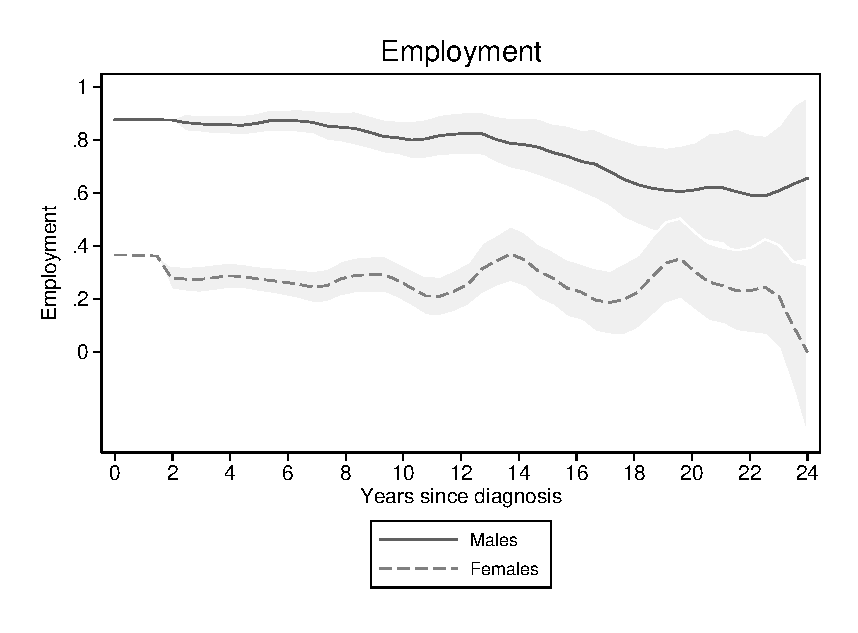
\includegraphics[width=0.5\columnwidth]{figures/lpoly_works_diabetesduration.eps}\\
%DIFDELCMD < \footnotesize{The dotted lines around the main line show 95\% confidence intervals.}
%DIFDELCMD < \end{center}
%DIFDELCMD < \end{figure}
%DIFDELCMD < \FloatBarrier
%DIFDELCMD < \begin{figure}[h!]
%DIFDELCMD < %%%
%DIFDELCMD < \caption{%
{%DIFAUXCMD
%DIFDELCMD < \label{fig:Kernel-weighted-local-polynomial_wage}%%%
\DIFdelFL{Kernel-weighted local
polynomial regression of log hourly wages on diabetes duration.}}%DIFAUXCMD
%DIF < 
%DIFDELCMD < \begin{center}
%DIFDELCMD < 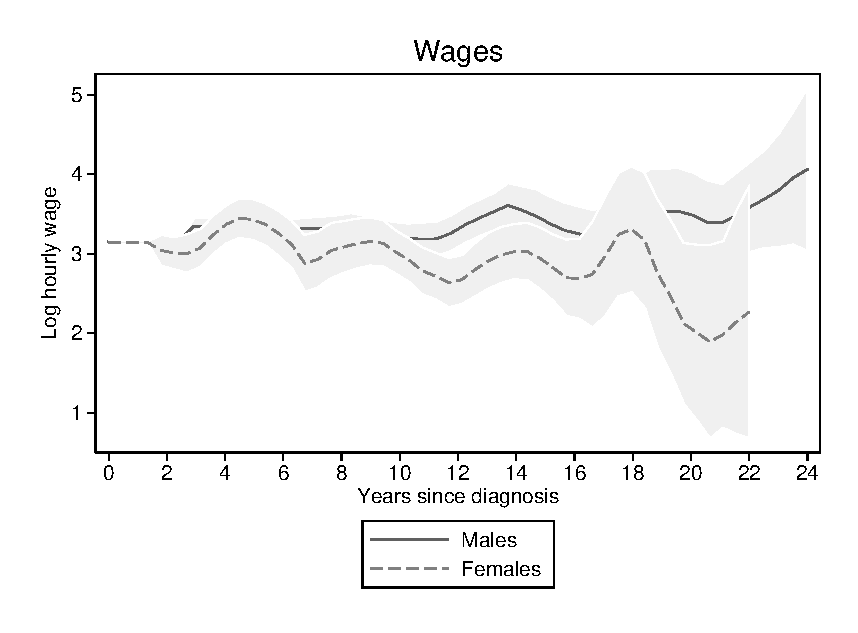
\includegraphics[width=0.5\columnwidth]{figures/lpoly_wage_diabetesduration.eps}\\
%DIFDELCMD < \footnotesize{The dotted lines around the main line show 95\% confidence intervals.}
%DIFDELCMD < \end{center}
%DIFDELCMD < \end{figure}
%DIFDELCMD < 

%DIFDELCMD < \begin{figure}[h!]
%DIFDELCMD < %%%
%DIFDELCMD < \caption{%
{%DIFAUXCMD
%DIFDELCMD < \label{fig:Kernel-weighted-local-polynomial_workhrs}%%%
\DIFdelFL{Kernel-weighted local
polynomial regression of working hours on diabetes duration.}}%DIFAUXCMD
%DIF < 
%DIFDELCMD < \begin{center}
%DIFDELCMD < 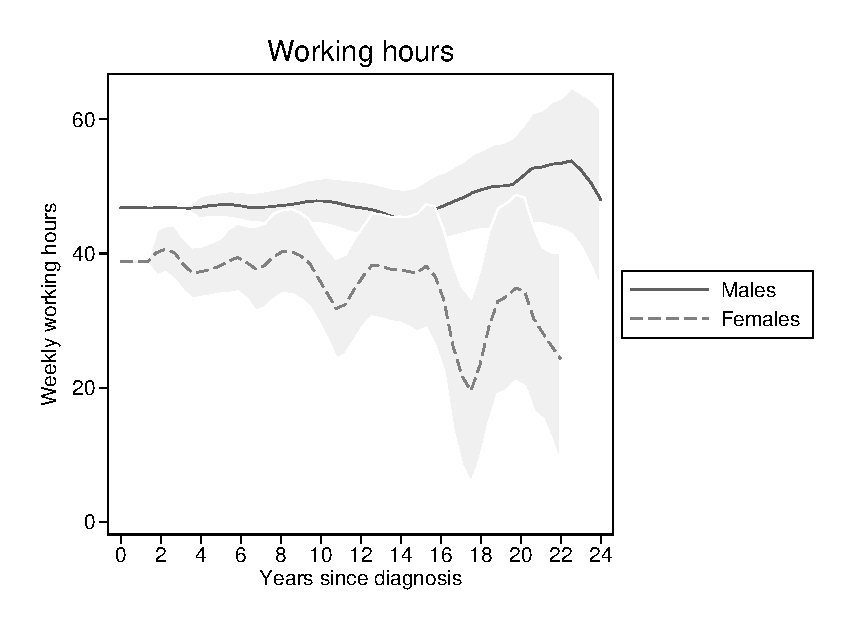
\includegraphics[width=0.5\columnwidth]{figures/lpoly_workhrs_diabetesduration.eps}%%%
\DIFdelendFL \DIFaddbeginFL 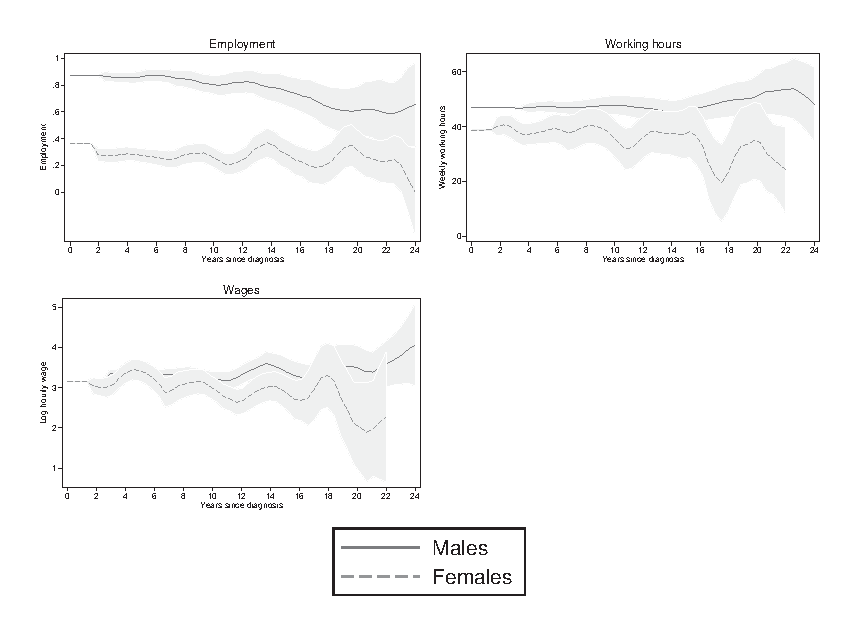
\includegraphics[width=\linewidth]{figures/lpoly_combined.eps}\DIFaddendFL \\
\DIFdelbeginFL %DIFDELCMD < \footnotesize{The dotted lines around the main line show 95\% confidence intervals.}
%DIFDELCMD < %%%
\DIFdelendFL \DIFaddbeginFL \footnotesize{\textit{Notes} The dashed lines show 95\% confidence interval.}
\DIFaddendFL \end{center}
\end{figure}
\DIFdelbegin %DIFDELCMD < \FloatBarrier
%DIFDELCMD < %%%
\DIFdelend 

\DIFdelbegin \DIFdel{Table \ref{tab:Self-reported-diabetes-duration} presents the results of the linear and non-linear duration models (for which we created the following splines to capture the immediate, intermediate and long-term relationships:0--4,
5--11, 12--19 and  20+), starting with the results of the cross-sectional }%DIFDELCMD < \ac{LPM}%%%
\DIFdel{, followed by the pooled }%DIFDELCMD < \ac{LPM} %%%
\DIFdel{and then the }%DIFDELCMD < \ac{FE} %%%
\DIFdel{model as specified in Eq. (\ref{eq:duration_linear} ) and Eq. (\ref{eq:splines})}\DIFdelend \DIFaddbegin \DIFadd{Tables \ref{tab:Self-reported-diabetes-duration_employ} and  \ref{tab:Self-reported-diabetes-duration_wage} present the estimation results for equations \ref{eq:duration_linear} and \ref{eq:splines}}\DIFaddend .

\DIFdelbegin \DIFdel{For employment probabilities the results indicate a yearly reduction in male employment probability throughout}\DIFdelend \DIFaddbegin \DIFadd{The results in Table \ref{tab:Self-reported-diabetes-duration_employ} panel A show that male employment probabilities fall every year in all models, with the biggest effects in the }\ac{FE} \DIFadd{model}\DIFaddend . For women\DIFaddbegin \DIFadd{, }\DIFaddend the coefficient shows a reduction of up to almost 1 \DIFdelbegin %DIFDELCMD < \ac{p.p.} %%%
\DIFdel{per year , though the association is not as strong }\DIFdelend \DIFaddbegin \DIFadd{percentage points per year }\DIFaddend in the \ac{FE} model\DIFdelbegin \DIFdel{. The coefficients in the spline modelsprovide some evidence for an immediate effect of diabetes, which then levels off for some time after which it becomes stronger again. Nonetheless, for males and particularly females, the coefficients are quite imprecisely measured}\DIFdelend \DIFaddbegin \DIFadd{, though its statistical significance is lower than in the }\ac{OLS} \DIFadd{models}\DIFaddend . 

\DIFdelbegin %DIFDELCMD < \begin{table}
%DIFDELCMD < %%%
\DIFdelend \DIFaddbegin \begin{table}[!ht]
\DIFaddendFL \caption{\DIFdelbeginFL %DIFDELCMD < \label{tab:Self-reported-diabetes-duration}%%%
\DIFdelendFL \DIFaddbeginFL \label{tab:Self-reported-diabetes-duration_employ}\DIFaddendFL Relationship between self-reported years since diagnosis and \DIFdelbeginFL \DIFdelFL{labor market outcomes }\DIFdelendFL \DIFaddbeginFL \DIFaddFL{employment probabilities }\DIFaddendFL using continuous duration and duration splines.}
\begin{center}
%DIF < \resizebox{\textwidth}{!}{%
\DIFdelbeginFL %DIFDELCMD < \begin{adjustbox}{max width=\textwidth}
%DIFDELCMD < %%%
\DIFdelendFL %DIF > \resizebox{\linewidth}{!}{%
\DIFaddbeginFL \begin{adjustbox}{max width=\linewidth}
\DIFaddendFL \begin{threeparttable}

{
\def\sym#1{\ifmmode^{#1}\else\(^{#1}\)\fi}
\begin{tabular}{l*{6}{S
S}}
\toprule
                &\multicolumn{3}{c}{Males}                               &\multicolumn{3}{c}{Females}                             \\\cmidrule(lr){2-4}\cmidrule(lr){5-7}
                &\multicolumn{1}{c}{(1)}&\multicolumn{1}{c}{(2)}&\multicolumn{1}{c}{(3)}&\multicolumn{1}{c}{(4)}&\multicolumn{1}{c}{(5)}&\multicolumn{1}{c}{(6)}\\
                  &\DIFdelbeginFL %DIFDELCMD < \multicolumn{1}{c}{OLS (wave 3)}%%%
\DIFdelendFL \DIFaddbeginFL \multicolumn{1}{c}{OLS}\DIFaddendFL &\DIFdelbeginFL %DIFDELCMD < \multicolumn{1}{c}{Pooled OLS}%%%
\DIFdelendFL \DIFaddbeginFL \multicolumn{1}{c}{OLS}\DIFaddendFL &\multicolumn{1}{c}{FE}&\DIFdelbeginFL %DIFDELCMD < \multicolumn{1}{c}{OLS (wave 3)}%%%
\DIFdelendFL \DIFaddbeginFL \multicolumn{1}{c}{OLS}\DIFaddendFL &\DIFdelbeginFL %DIFDELCMD < \multicolumn{1}{c}{Pooled OLS}%%%
\DIFdelendFL \DIFaddbeginFL \multicolumn{1}{c}{OLS}\DIFaddendFL &\multicolumn{1}{c}{FE}\\
                                \DIFdelbeginFL %DIFDELCMD < \addlinespace
%DIFDELCMD < \midrule %%%
\DIFdelendFL &\DIFdelbeginFL %DIFDELCMD < \multicolumn{6}{c}{\emph{Employment probabilities}} %%%
\DIFdelendFL \DIFaddbeginFL \multicolumn{1}{c}{(Wave 3)}&\multicolumn{1}{c}{(Pooled)}&\multicolumn{1}{c}{}&\multicolumn{1}{c}{(Wave 3)}&\multicolumn{1}{c}{(Pooled)}&\multicolumn{1}{c}{}\DIFaddendFL \\
\DIFaddbeginFL \midrule
\DIFaddendFL \addlinespace
Panel A: \DIFaddbeginFL \DIFaddFL{linear }\DIFaddendFL &&&&&&\\
Diabetes duration \DIFdelbeginFL \DIFdelFL{(linear)}\DIFdelendFL &   -.008\sym{***}&    -.007\sym{***}&    -.017\sym{***}&    -.005\sym{***}&    -.004\sym{***}&    -.009\sym{*}  \\
                &   (.002)         &   (.002)         &   (.006)         &   (.002)         &   (.001)         &   (.005)         \\
                \DIFaddbeginFL 

\midrule
                \DIFaddFL{Hausman test    }&                  &                  &  \DIFaddFL{153.024         }&                  &                  &  \DIFaddFL{200.073         }\\
                \hspace*{10mm} \DIFaddFL{p-value         }&                  &                  &     \DIFaddFL{.000         }&                  &                  &     \DIFaddFL{.000         }\\
\DIFaddendFL \midrule
\addlinespace
Panel B: \DIFaddbeginFL \DIFaddFL{splines}\DIFaddendFL &&&&&&\\
Diabetes duration \DIFdelbeginFL \DIFdelFL{(splines)}\DIFdelendFL &&&&&&\\
\hspace*{10mm}0--4&    -.007         &    -.007         &    -.026\sym{*}  &    -.010         &    -.015\sym{**} &    -.017         \\
                &   (.007)         &   (.006)         &   (.014)         &   (.007)         &   (.006)         &   (.016)         \\
\hspace*{10mm}5--11&     .000         &    -.003         &    -.003         &    -.004         &     .004         &    -.003         \\
                &   (.009)         &   (.006)         &   (.009)         &   (.008)         &   (.006)         &   (.008)         \\
\hspace*{10mm}12--20&  -.030\sym{**} &    -.017\sym{*}  &    -.029\sym{*}  &     .005         &    -.004         &    -.014         \\
                &   (.012)         &   (.010)         &   (.016)         &   (.008)         &   (.006)         &   (.011)         \\
\hspace*{10mm}> 20&     .011         &     .007         &    -.046\sym{*}  &    -.010\sym{*}  &    -.003         &    -.015         \\
                &   (.016)         &   (.014)         &   (.028)         &   (.006)         &   (.003)         &   (.018)         \\
\midrule
\DIFaddbeginFL \DIFaddFL{Hausman test    }&                  &                  &  \DIFaddFL{161.953         }&                  &                  &  \DIFaddFL{198.692         }\\
\hspace*{10mm} \DIFaddFL{p-value         }&                  &                  &     \DIFaddFL{.000         }&                  &                  &     \DIFaddFL{.000         }\\
\DIFaddendFL N               &     8217         &    16292         &    16292         &    10467         &    22407         &    22407         \\
\DIFdelbeginFL %DIFDELCMD < \midrule 
%DIFDELCMD < \addlinespace
%DIFDELCMD < %%%
\DIFdelendFL \DIFaddbeginFL \bottomrule
\end{tabular}
\begin{tablenotes}
\item \footnotesize \textit{\DIFaddFL{Notes}} \DIFaddFL{The table presents the results of three estimation methods. Panel A presents the results of the linear specifications. Panel B presents the results of the non-linear specifications. Robust standard errors in parentheses. Other control variables: state dummies, urbanization dummies, education dummies, married dummy, number children < 6, wealth, age squared and calendar year dummies. The OLS and pooled OLS models additionally control for age. }\sym{*} \DIFaddFL{\(p<0.10\), }\sym{**} \DIFaddFL{\(p<0.05\), }\sym{***} \DIFaddFL{\(p<0.01\).
}\end{tablenotes}
}
\end{threeparttable}
\end{adjustbox}
\end{center}
\end{table}

\DIFadd{Panel B of Table \ref{tab:Self-reported-diabetes-duration_employ} shows the estimates when using a spline function. Focusing on the }\ac{FE} \DIFadd{results, the coefficients provide some evidence for an immediate effect of diabetes, which then levels off for some time after which it becomes stronger again. However, standard errors are quite large.
}

\DIFadd{The results in Table \ref{tab:Self-reported-diabetes-duration_wage} indicate a reduction in female wages of about 7}\% \DIFadd{per year with diabetes in the }\ac{FE} \DIFadd{model. For men we find no consistent effect. The results of the non-linear specification in panel B of Table \ref{tab:Self-reported-diabetes-duration_wage} indicate that there may be a reduction in wages 5--11 years after the initial diagnosis for both men and women. We also find associations for women with more than 20 years of diabetes, but these estimates may be spurious due to the considerably reduced number of observations in this group.}\footnote{\DIFadd{There are only 9 and 3 observations for male and female wages with more than 20 years since diagnosis in wave 3, respectively, and 17 and 7 in the pooled sample, respectively. For male and female working hours there are 12 and 7 observations with more than 20 years since diagnosis in wave 3, respectively, and 20 and 12 for the pooled sample, respectively.}} \DIFadd{Interestingly, the reductions in wages found in the non-linear specification appear exactly at the time where employment probabilities are less affected. This could suggest that at this point reductions in productivity affect wages but are not so severe that they would cause job loss. 
}

\begin{table}[!ht]
\caption{\label{tab:Self-reported-diabetes-duration_wage}\DIFaddFL{Relationship between self-reported years since diagnosis and log hourly wage using continuous duration and duration splines.}}
\begin{center}
%DIF > \resizebox{\linewidth}{!}{%
\begin{adjustbox}{max width=\linewidth}
\begin{threeparttable}
{
\def\sym#1{\ifmmode^{#1}\else\(^{#1}\)\fi}
\begin{tabular}{l*{6}{S
S}}
\toprule
                \DIFaddendFL &\DIFdelbeginFL %DIFDELCMD < \multicolumn{6}{c}{\emph{Log hourly wage}} %%%
\DIFdelendFL \DIFaddbeginFL \multicolumn{3}{c}{Males}                               &\multicolumn{3}{c}{Females}                             \DIFaddendFL \\\DIFdelbeginFL %DIFDELCMD < \addlinespace
%DIFDELCMD < %%%
\DIFdelendFL \DIFaddbeginFL \cmidrule\DIFaddFL{(lr)}{\DIFaddFL{2-4}}\cmidrule\DIFaddFL{(lr)}{\DIFaddFL{5-7}}
                &\multicolumn{1}{c}{(1)}&\multicolumn{1}{c}{(2)}&\multicolumn{1}{c}{(3)}&\multicolumn{1}{c}{(4)}&\multicolumn{1}{c}{(5)}&\multicolumn{1}{c}{(6)}\\
                &\multicolumn{1}{c}{OLS}&\multicolumn{1}{c}{OLS}&\multicolumn{1}{c}{FE}&\multicolumn{1}{c}{OLS}&\multicolumn{1}{c}{OLS}&\multicolumn{1}{c}{FE}\\
                 &\multicolumn{1}{c}{(wave 3)}&\multicolumn{1}{c}{(pooled)}&\multicolumn{1}{c}{}&\multicolumn{1}{c}{(wave 3)}&\multicolumn{1}{c}{(pooled)}&\multicolumn{1}{c}{}\\
\midrule
\DIFaddendFL Panel A: \DIFaddbeginFL \DIFaddFL{linear }\DIFaddendFL &&&&&&\\
Diabetes duration\DIFdelbeginFL \DIFdelFL{(linear)}\DIFdelendFL &  .001         &     .010\sym{**} &    -.019         &    -.014\sym{*}  &    -.009         &    -.073\sym{**} \\
                &   (.006)         &   (.005)         &   (.018)         &   (.008)         &   (.008)         &   (.029)         \\
\midrule                
\DIFaddbeginFL \DIFaddFL{Hausman test    }&                  &                  &  \DIFaddFL{838.213         }&                  &                  &   \DIFaddFL{93.232         }\\
\hspace*{10mm} \DIFaddFL{p-value         }&                  &                  &     \DIFaddFL{.000         }&                  &                  &     \DIFaddFL{.000         }\\                
\midrule
\DIFaddendFL \addlinespace
Panel B: \DIFaddbeginFL \DIFaddFL{splines}\DIFaddendFL &&&&&&\\
Diabetes duration\DIFdelbeginFL \DIFdelFL{(splines)}\DIFdelendFL &&&&&&\\
\hspace*{10mm}0--4&      .034\sym{*}  &     .046\sym{***}&     .033         &     .027         &     .030         &     .015         \\
                &   (.017)         &   (.016)         &   (.055)         &   (.031)         &   (.026)         &   (.138)         \\
\hspace*{10mm}5--11&    -.041\sym{*}  &    -.037\sym{**} &    -.055\sym{*}  &    -.039         &    -.034         &    -.101\sym{*}  \\
                &   (.021)         &   (.018)         &   (.033)         &   (.030)         &   (.024)         &   (.056)         \\
\hspace*{10mm}12--20&      0.015         &     .044         &     .062         &    -.032         &    -.071\sym{*}  &    -.051         \\
                &   (.033)         &   (.029)         &   (.056)         &   (.042)         &   (.039)         &   (.047)         \\
\hspace*{10mm}> 20&     .053         &     .014         &    -.111         &    -.007         &     .041\sym{***}&    -.204\sym{***}\\
                &   (.054)         &   (.040)         &   (.104)         &   (.028)         &   (.015)         &   (.053)         \\
\midrule
\DIFaddbeginFL \DIFaddFL{Hausman test    }&                  &                  & \DIFaddFL{1037.290         }&                  &                  &   \DIFaddFL{96.266         }\\
\hspace*{10mm} \DIFaddFL{p-value         }&                  &                  &     \DIFaddFL{.000         }&                  &                  &     \DIFaddFL{.000         }\\
\DIFaddendFL N               &     5509         &    10767         &    10767         &     2874         &     5741         &     5741         \\
\DIFdelbeginFL %DIFDELCMD < \midrule
%DIFDELCMD < \addlinespace
%DIFDELCMD < %%%
\DIFdelendFL \DIFaddbeginFL \bottomrule
\end{tabular}
\begin{tablenotes}
\item \footnotesize \textit{\DIFaddFL{Notes}} \DIFaddFL{The table presents the results of three estimation methods for log hourly wages. Panel A presents the results of the linear specifications. Panel B presents the results of the non-linear specifications. Robust standard errors in parentheses. Other control variables: state dummies, urbanization dummies, education dummies, married dummy, number children < 6, wealth, age squared, calendar year dummies, type of work (agricultural and self employed with dependent non-agricultural wage employment as the base) and health insurance status. The OLS and pooled OLS models additionally control for age. }\sym{*} \DIFaddFL{\(p<0.10\), }\sym{**} \DIFaddFL{\(p<0.05\), }\sym{***} \DIFaddFL{\(p<0.01\).
}\end{tablenotes}
}
\end{threeparttable}
\end{adjustbox}
\end{center}
\end{table}

\DIFadd{The estimation results in Table \ref{tab:Self-reported-diabetes-duration_hours} indicate that there appears to be no consistent relationship between working hours and time since being diagnosed with diabetes, neither for men nor for women.
}


\DIFadd{Taken together, these results suggest a fairly constant decrease in the probability of employment for both men and women and in earnings for women, which contrast with estimates for the USA }\parencite{Minor2013}\DIFadd{, where no such relationship is observed.  \textcite{Minor2013} finds a reduction in employment probabilities of 82 percentage points for females after 11 to 15 years and a reduction of 60 percentage points for males after 2-5 years, indicating very large employment penalties, in particular in comparison to our results for Mexico. However, the non-linear results we presented are not directly comparable to these estimates as Minor used pooled cross-sectional data, constructed dummy variables instead of splines and used different duration groups. When we use a similar model to \textcite{Minor2013}  the results confirm that the employment effects are substantially less negative in Mexico than in US. For men they reduce with 6-12}\% \DIFadd{in the first 2 and 4 years respectively---depending on the specification used, and some increase in the following years. We find no immediate effect of diagnosis for women, but effects do emerge after about 2 years and tend to increase somewhat over time.}\footnote{\DIFadd{Following \textcite{Minor2013} we find a significant reduction in employment probabilities throughout, regardless of whether we use our duration groups to construct the dummies or the duration groups used by \textcite{Minor2013}.}} 

\DIFadd{The increasing adverse effects of diabetes over time are plausible in that as time lived with diabetes evolves, complications associated with diabetes tend to become more frequent and more severe }\parencite{Adler2003}\DIFadd{. Looking at wages as our labor market outcome, we uncover some adverse effects for females, indicating a sizeable reduction with time since diagnosis.
}


\begin{table}[p]
\caption{\label{tab:Self-reported-diabetes-duration_hours}\DIFaddFL{Relationship between self-reported years since diagnosis and weekly working hours using continuous duration and duration splines.}}
\begin{center}
%DIF > \resizebox{\linewidth}{!}{%
\begin{adjustbox}{max width=\linewidth}
\begin{threeparttable}
{
\def\sym#1{\ifmmode^{#1}\else\(^{#1}\)\fi}
\begin{tabular}{l*{6}{S
S}}
\toprule
                \DIFaddendFL &\DIFdelbeginFL %DIFDELCMD < \multicolumn{6}{c}{\emph{Weekly working hours}}%%%
\DIFdelendFL \DIFaddbeginFL \multicolumn{3}{c}{Males}                               &\multicolumn{3}{c}{Females}                             \DIFaddendFL \\\DIFdelbeginFL %DIFDELCMD < \addlinespace
%DIFDELCMD < %%%
\DIFdelendFL \DIFaddbeginFL \cmidrule\DIFaddFL{(lr)}{\DIFaddFL{2-4}}\cmidrule\DIFaddFL{(lr)}{\DIFaddFL{5-7}}
                &\multicolumn{1}{c}{(1)}&\multicolumn{1}{c}{(2)}&\multicolumn{1}{c}{(3)}&\multicolumn{1}{c}{(4)}&\multicolumn{1}{c}{(5)}&\multicolumn{1}{c}{(6)}\\
                &\multicolumn{1}{c}{OLS}&\multicolumn{1}{c}{OLS}&\multicolumn{1}{c}{FE}&\multicolumn{1}{c}{OLS}&\multicolumn{1}{c}{OLS}&\multicolumn{1}{c}{FE}\\
                 &\multicolumn{1}{c}{(wave 3)}&\multicolumn{1}{c}{(pooled)}&\multicolumn{1}{c}{}&\multicolumn{1}{c}{(wave 3)}&\multicolumn{1}{c}{(pooled)}&\multicolumn{1}{c}{}\\
\midrule
\DIFaddendFL Panel A: \DIFaddbeginFL \DIFaddFL{linear }\DIFaddendFL &&&&&&\\
Diabetes duration \DIFdelbeginFL \DIFdelFL{(linear)}\DIFdelendFL & .069         &     .048         &     .181         &    -.020         &    -.124         &     .208         \\
                &   (.124)         &   (.102)         &   (.330)         &   (.187)         &   (.127)         &   (.652)         \\
\midrule
\DIFaddbeginFL \DIFaddFL{Hausman test    }&                  &                  &  \DIFaddFL{704.904         }&                  &                  &  \DIFaddFL{107.709         }\\
\hspace*{10mm} \DIFaddFL{p-value         }&                  &                  &     \DIFaddFL{.000         }&                  &                  &     \DIFaddFL{.000         }\\
\midrule
\DIFaddendFL \addlinespace
Panel B: \DIFaddbeginFL \DIFaddFL{splines }\DIFaddendFL &&&&&&\\
Diabetes duration \DIFdelbeginFL \DIFdelFL{(splines)}\DIFdelendFL &&&&&&\\
\hspace*{10mm}0--4&      -.033         &    -.233         &     .709         &     .739         &     .470         &    2.014         \\
                &   (.421)         &   (.325)         &   (.938)         &   (.645)         &   (.586)         &  (2.947)         \\
\hspace*{10mm}5--11&  .269         &     .338         &    -.218         &    -.410         &    -.479         &    -.508         \\
                &   (.539)         &   (.399)         &   (.568)         &   (.728)         &   (.553)         &  (1.020)         \\
\hspace*{10mm}12--20&    .209         &     .137         &     .698         &    -.164         &    -.051         &    -.402         \\
                &   (.730)         &   (.538)         &   (.945)         &   (.995)         &   (.700)         &  (1.207)         \\
\hspace*{10mm}> 20&  -1.300         &    -.768         &     .039         &    -.499         &    -.418         &    8.117\sym{***}\\
                &   (.944)         &   (.930)         &  (2.184)         &   (.930)         &   (.305)         &  (1.612)         \\
\midrule
\DIFaddbeginFL \DIFaddFL{Hausman test    }&                  &                  &  \DIFaddFL{724.225         }&                  &                  &  \DIFaddFL{112.627         }\\
\hspace*{10mm} \DIFaddFL{p-value         }&                  &                  &     \DIFaddFL{.000         }&                  &                  &     \DIFaddFL{.000         }\\
\DIFaddendFL N               &     6807         &    \DIFdelbeginFL \DIFdelFL{13579         }\DIFdelendFL \DIFaddbeginFL \DIFaddFL{13581         }\DIFaddendFL &    \DIFdelbeginFL \DIFdelFL{13579         }\DIFdelendFL \DIFaddbeginFL \DIFaddFL{13581         }\DIFaddendFL &     3591         &     7383         &     7383         \\
\bottomrule
\end{tabular}
\begin{tablenotes}
\item \DIFaddbeginFL \footnotesize \textit{\DIFaddFL{Notes}} \DIFaddendFL The table presents the results of three estimation methods for \DIFdelbeginFL \DIFdelFL{the three dependent variables: employment probabilities, log hourly wages and }\DIFdelendFL weekly working hours. Panel A presents the results of the linear specifications. Panel B presents the results of the non-linear specifications. Robust standard errors in parentheses. Other control variables: state dummies, urbanization dummies, education dummies, married dummy, number children < 6, wealth, age squared\DIFdelbeginFL \DIFdelFL{and }\DIFdelendFL \DIFaddbeginFL \DIFaddFL{, }\DIFaddendFL calendar year dummies\DIFdelbeginFL \DIFdelFL{. The wage and working hour models additionally control for }\DIFdelendFL \DIFaddbeginFL \DIFaddFL{, }\DIFaddendFL type of work (agricultural and self employed with dependent non-agricultural wage employment as the base) and \DIFdelbeginFL \DIFdelFL{for }\DIFdelendFL health insurance status. The OLS and pooled OLS models additionally control for age. \sym{*} \(p<0.10\), \sym{**} \(p<0.05\), \sym{***} \(p<0.01\).
\end{tablenotes}
}
\end{threeparttable}
\end{adjustbox}
\end{center}
\end{table}

\DIFdelbegin \DIFdel{Turning to wages, the }%DIFDELCMD < \ac{FE} %%%
\DIFdel{model indicates a reduction in female wages of about 7}%DIFDELCMD < \% %%%
\DIFdel{per year with diabetes. For men we find no consistent effect. The results of the non-linear specification indicate that there may be a reduction in wages 5--11 years after the initial diagnosis. We also find associations for women with more than 20 years of diabetes, but these estimates may be spurious due to the considerably reduced number of observations in this group.}\footnote{\DIFdel{There are only 9 and 3 observations for male and female wages with more than 20 years since diagnosis in wave 3, respectively, and similarly 17 and 7 in the pooled sample, respectively. For male and female working hours there are 12 and 7 observations with more than 20 years since diagnosis in wave 3, respectively, and 20 and 12 for the pooled sample, respectively.}}%DIFAUXCMD
\addtocounter{footnote}{-1}%DIFAUXCMD
\DIFdel{. There appears to be no consistent relationship between working hours and time since being diagnosed with diabetes.
   }%DIFDELCMD < 

%DIFDELCMD < %%%
\DIFdel{Overall these results suggest a fairly constant decrease in the probability of employment for both men and women and in earnings for women, which contrast with estimates for the }%DIFDELCMD < \ac{USA} \parencite{Minor2013}%%%
\DIFdel{, where no such linear relationship is observed.  \textcite{Minor2013} finds a reduction in employment probabilities of 82 }%DIFDELCMD < \ac{p.p.} %%%
\DIFdel{for females after 11 to 15 years and a reduction of 60 }%DIFDELCMD < \ac{p.p.} %%%
\DIFdel{for males after 2-5 years, indicating very large employment penalties, in particular in comparison to our results for Mexico. However, our non-linear results are not directly comparable to these estimates as Minor used pooled cross-sectional data, constructed dummy variables instead of splines and used different duration groups.}\footnote{\DIFdel{We estimated a comparable model to that of \textcite{Minor2013} using dummy variables and find a significant reduction in employment chances throughout, regardless of whether we use our duration groups to construct the dummies or the duration groups used by \textcite{Minor2013}. For men, we find a significant reduction of about 6 to 12 }%DIFDELCMD < \ac{p.p.}%%%
\DIFdel{, depending on the used specification, in the first 2 and 4 years after diagnosis, respectively. In the following years the effect size tends to increase somewhat. For women, we find less evidence for an immediate effect of diagnosis, but effects do emerge after about 2 years of living with the disease and also increase somewhat over time. These results are available on request.}}
%DIFAUXCMD
\addtocounter{footnote}{-1}%DIFAUXCMD
\DIFdelend \FloatBarrier

\subsection{Cross-sectional biomarker analysis}


\DIFdelbegin \DIFdel{In this section we gain additional insights from using the biomarker data collected in the
third wave of the }%DIFDELCMD < \ac{MxFLS}%%%
\DIFdel{. As noted in section \ref{sec:Data}, these data enable us to identify respondents with
}%DIFDELCMD < \ac{HbA1c} %%%
\DIFdel{levels equal to or above the internationally recognized diabetes threshold of 6.5}%DIFDELCMD < \%%%%
\DIFdel{. This will allow the investigation of the direction of bias introduced when relying on self-reported diabetes only and when it is not possible to identify those unaware as well.
}%DIFDELCMD < 

%DIFDELCMD < %%%
\DIFdel{We first present }\DIFdelend \DIFaddbegin \DIFadd{Table \ref{tab:Biomarker_observations} presents }\DIFaddend a cross tabulation of self-reported diabetes and \DIFdelbegin \DIFdel{the results of the biomarker analysis (Table  \ref{tab:Biomarker_observations}). The table indicates }\DIFdelend \DIFaddbegin \DIFadd{biomarker results, indicating }\DIFaddend that 27\% of the sample have \ac{HbA1c} levels indicative of diabetes and 81\% of those self-reporting a diabetes diagnosis also have \ac{HbA1c} levels equal to or above the diabetes threshold. \DIFdelbegin \DIFdel{Overall, of the people with }\DIFdelend \DIFaddbegin \DIFadd{The cell percentages in the table underline the large proportion of false negatives (18}\%\DIFadd{). The 3}\% \DIFadd{with self-reported diabetes but biomarker levels below the diabetes threshold could be interpreted as false positives, however, likely a large proportion has received a diabetes diagnosis but has achieved blood glucose levels below the diabetes threshold thanks to treatment and lifestyle changes. Of the respondents who tested positive for }\DIFaddend diabetes according to \DIFaddbegin \DIFadd{the }\DIFaddend biomarker analysis, 32\% self-report a diagnosis, while 68\% do not. \DIFaddbegin \DIFadd{There are no considerable differences to the presented proportions in Table \ref{tab:Biomarker_observations} if we look at men and women separately and we therefore do not show these results here. 
}\DIFaddend 


\DIFdelbegin %DIFDELCMD < \begin{table}[h!]
%DIFDELCMD < %%%
\DIFdelend \DIFaddbegin \begin{table}[ht]
\DIFaddendFL \caption{\label{tab:Biomarker_observations}Number of observations with diabetes (HbA1c $\geq 6.5\%$) and self-reported diabetes.}
\begin{center}
\DIFdelbeginFL %DIFDELCMD < \begin{adjustbox}{max width=\textwidth}
%DIFDELCMD < %%%
\DIFdelendFL \DIFaddbeginFL \begin{adjustbox}{max width=\linewidth}
\DIFaddendFL \begin{threeparttable}
{
\def\sym#1{\ifmmode^{#1}\else\(^{#1}\)\fi}
\begin{tabular}{l*{3}{S S}}
\toprule
            &\multicolumn{1}{c}{$HbA1c < 6.5\%$}&\multicolumn{1}{c}{HbA1c $\geq 6.5\%$}&\multicolumn{1}{c}{Total}\\
\midrule
No self-reported diabetes \DIFaddbeginFL \DIFaddFL{(N) }\DIFaddendFL & 4544 & 1181 & 5725 &  \\
\DIFaddbeginFL \hspace*{10mm}\DIFaddFL{Row  }\% \DIFaddendFL & 79\% & 21\% & 100\% &  \\
\DIFaddbeginFL \hspace*{10mm}\DIFaddFL{Column }\% \DIFaddendFL & 97\% & 68\% & 89\% &  \\
\DIFaddbeginFL \hspace*{10mm}\DIFaddFL{Cell }\% & \DIFaddFL{71}\% & \DIFaddFL{18}\% & \DIFaddFL{z }& \\
\DIFaddendFL Self-reported diabetes \DIFaddbeginFL \DIFaddFL{(N) }\DIFaddendFL & 129 & 554 & 683 &  \\
\DIFaddbeginFL \hspace*{10mm}\DIFaddFL{Row }\%  \DIFaddendFL & 19\% & 81\% & 100\% &  \\
\DIFaddbeginFL \hspace*{10mm}\DIFaddFL{Column }\% \DIFaddendFL & 3\% & 32\% & 11\% &  \\
\DIFdelbeginFL \DIFdelFL{Total }\DIFdelendFL \DIFaddbeginFL \hspace*{10mm}\DIFaddFL{Cell }\% & \DIFaddFL{2}\% & \DIFaddFL{9}\% & \DIFaddFL{z }& \\
\DIFaddFL{Total (N) }\DIFaddendFL & 4673 & 1735 & 6408 &  \\
\DIFaddbeginFL \hspace*{10mm}\DIFaddFL{Row }\% \DIFaddendFL & 73\% & 27\% & 100\% &  \\
\DIFaddbeginFL \hspace*{10mm}\DIFaddFL{Column }\%  \DIFaddendFL & 100\% & 100\% & 100\% &  \\
\DIFaddbeginFL \hspace*{10mm}\DIFaddFL{Cell }\% & \DIFaddFL{x }& \DIFaddFL{y }& \DIFaddFL{z }& \\  
\DIFaddendFL \bottomrule
\end{tabular}
\begin{tablenotes}
\item
\DIFdelbeginFL \DIFdelFL{The first row of each category presents absolute values, the second row row percentages and the third row column percentages.
}\DIFdelendFL \end{tablenotes}
}
\end{threeparttable}
\end{adjustbox}
\end{center}
\end{table}

\DIFdelbegin %DIFDELCMD < \FloatBarrier
%DIFDELCMD < 

%DIFDELCMD < %%%
\DIFdel{To further investigate the relationship of self-reported and biomarker tested diabetes, we estimate the models presented in section \ref{sec:Biomarker Strategy}}\DIFdelend \DIFaddbegin \DIFadd{Table \ref{tab:Biomarker_results} presents the results from estimating equations \ref{eq:diab_sr}, \ref{eq:diab} and \ref{eq:diab_ud}}\DIFaddend .  
The results in columns 1 and 2 of Table \ref{tab:Biomarker_results} show that the earlier \DIFdelbegin \DIFdel{results }\DIFdelend \DIFaddbegin \DIFadd{longitudinal results using self-reported diabetes }\DIFaddend are robust for the biomarker sample. The coefficients in column 3 and 4 indicate that the \DIFdelbegin \DIFdel{associations with employment probabilities are }\DIFdelend \DIFaddbegin \DIFadd{relationship becomes }\DIFaddend much weaker when using diabetes defined by the biomarker instead of self-reported diabetes.\footnote{We also created a dummy variable that additionally to measured diabetes accounted for those with a self-reported diabetes diagnosis but \DIFdelbegin \DIFdel{biomaker }\DIFdelend \DIFaddbegin \DIFadd{biomarker }\DIFaddend levels below the diabetes threshold. This \DIFdelbegin \DIFdel{allowed us }\DIFdelend \DIFaddbegin \DIFadd{is of interest because those who suffer from diabetes but manage }\DIFaddend to \DIFdelbegin \DIFdel{investigate }\DIFdelend \DIFaddbegin \DIFadd{control their sugar levels may obtain test results outside }\DIFaddend the \DIFdelbegin \DIFdel{effect for }\DIFdelend \DIFaddbegin \DIFadd{diabetes range.  If one would choose to believe there is no misreporting, this can be seen as representing }\DIFaddend the entire diabetes population. The coefficients and their statistical significance are only marginally different to those presented in columns 3 and 4 of Table \DIFdelbegin \DIFdel{\ref{tab:Biomarker_results}}\DIFdelend \DIFaddbegin \DIFadd{8}\DIFaddend , which is why we do not present them here.} In columns 5 and 6 \DIFaddbegin \DIFadd{of Table \ref{tab:Biomarker_results}}\DIFaddend , obtained from estimating \DIFdelbegin \DIFdel{Eq. }\DIFdelend \DIFaddbegin \DIFadd{equations }\DIFaddend \ref{eq:diab_ud}, the coefficient for the biomarker diabetes population \DIFdelbegin \DIFdel{$Dbio_i$ }\DIFdelend now reflects the effect of undiagnosed diabetes, as the regression includes a control for self-reported diabetes, revealing that \DIFdelbegin \DIFdel{undiagnosed diabetes is not associated with any of the labor outcomes . The coefficient for self-reported diabetes is marginally bigger in size for men and somewhat smaller for women compared to column 1 and 2, respectively. However, these differences are not statistically significant (p>0.1) using a Z-test, suggesting that not accounting for undiagnosed diabetes will likely leave the estimates of self-reported diabetes unbiased}\DIFdelend \DIFaddbegin \DIFadd{labor outcomes are not lower for those with undiagnosed diabetes}\DIFaddend . 

\DIFdelbegin %DIFDELCMD < \begin{table}[h!]
%DIFDELCMD < %%%
\DIFdelend \DIFaddbegin \begin{table}[h]
\DIFaddendFL \caption{\label{tab:Biomarker_results}Biomarker results}
\begin{center}
\begin{adjustbox}{max width=\linewidth}
\begin{threeparttable}
{
\def\sym#1{\ifmmode^{#1}\else\(^{#1}\)\fi}
\begin{tabular}{l*{6}{S
S}}
\toprule
                &\DIFdelbeginFL %DIFDELCMD < \multicolumn{2}{c}{Self-reported diabetes}    &\multicolumn{2}{c}{HbA1c $\geq$ 6.5}&\multicolumn{2}{c}{HbA1c $\geq$ 6.5 and self-reported d.}                 \\\cmidrule%%%
\DIFdelFL{(lr)}%DIFDELCMD < {%%%
\DIFdelFL{2-3}%DIFDELCMD < }\cmidrule%%%
\DIFdelFL{(lr)}%DIFDELCMD < {%%%
\DIFdelFL{4-5}%DIFDELCMD < }\cmidrule%%%
\DIFdelFL{(lr)}%DIFDELCMD < {%%%
\DIFdelFL{6-7}%DIFDELCMD < }
%DIFDELCMD <                 &%%%
\DIFdelendFL \multicolumn{1}{c}{(1)}&\multicolumn{1}{c}{(2)}&\multicolumn{1}{c}{(3)}&\multicolumn{1}{c}{(4)}&\multicolumn{1}{c}{(5)}&\multicolumn{1}{c}{(6)}\\
                &\multicolumn{1}{c}{Males}&\multicolumn{1}{c}{Females}&\multicolumn{1}{c}{Males}&\multicolumn{1}{c}{Females}&\multicolumn{1}{c}{Males}&\multicolumn{1}{c}{Females}\\
\midrule
\multicolumn{7}{l}{\hspace*{10mm}\textbf{Dependent variable: Employment}} \\
Self-reported diabetes&   -.051\sym{**} &    -.044\sym{*}  &                  &                  &    -.053\sym{**} &    -.032         \\
                &   (.026)         &   (.023)         &                  &                  &   (.026)         &   (.026)         \\
HbA1c $\geq$ 6.5&                  &                  &    -.012         &    -.031\sym{*}  &     .003         &    -.022         \\
                &                  &                  &   (.016)         &   (.018)         &   (.017)         &   (.019)         \\
\midrule
N               &\multicolumn{1}{S}{2785}         &\multicolumn{1}{S}{3623}         &\multicolumn{1}{S}{2785}         &\multicolumn{1}{S}{3623}         &\multicolumn{1}{S}{2785}         &\multicolumn{1}{S}{3623}         \\
\midrule
\multicolumn{7}{l}{\hspace*{10mm}\textbf{Dependent variable: Log hourly wages}} \\ 
\addlinespace
Self-reported diabetes&    -.010         &    -.040         &                  &                  &    -.006         &    -.010         \\
                &   (.065)         &   (.113)         &                  &                  &   (.078)         &   (.119)         \\
HbA1c $\geq$ 6.5&                  &                  &    -.007         &    -.057         &    -.006         &    -.055         \\
                &                  &                  &   (.044)         &   (.070)         &   (.049)         &   (.075)         \\
\midrule
N               &\multicolumn{1}{S}{1803}         &\multicolumn{1}{S}{884}         &\multicolumn{1}{S}{1803}         &\multicolumn{1}{S}{884}         &\multicolumn{1}{S}{1803}         &\multicolumn{1}{S}{884}         \\
\midrule
\multicolumn{7}{l}{\hspace*{10mm}\textbf{Dependent variable: Weekly working hours}} \\ 
\addlinespace
Self-reported diabetes&   -.293         &    -.751         &                  &                  &    -.286         &   -1.566         \\
                &  (1.305)         &  (2.178)         &                  &                  &  (1.419)         &  (2.351)         \\
HbA1c $\geq$ 6.5&                  &                  &    -.088         &    1.153         &    -.012         &    1.525         \\
                &                  &                  &   (.844)         &  (1.462)         &   (.925)         &  (1.565)         \\
\bottomrule
\end{tabular}
\begin{tablenotes}
\item \DIFaddbeginFL \footnotesize \textit{\DIFaddFL{Notes}} \DIFaddendFL Community level fixed effects. Robust standard errors in parentheses. Other control variables: age, age squared, state dummies, urbanization dummies, education dummies, married dummy, number children < 6 and wealth. Calender year dummies are included as data collection for the third wave was stretched out over several years. The wage and working hour models additionally control for type of work (agricultural and self employed with non-agricultural wage employment as the base) and for health insurance status. \sym{*} \(p<0.10\), \sym{**} \(p<0.05\), \sym{***} \(p<0.01\).
\end{tablenotes}
}
\end{threeparttable}
\end{adjustbox}
\end{center}
\end{table}

\DIFdelbegin \DIFdel{As discussed earlier, differences in effects between self-reported diabetes and those undiagnosed are likely to stem }\DIFdelend \DIFaddbegin \DIFadd{To explore whether this stems }\DIFaddend from selection into the diagnosed population \DIFdelbegin \DIFdel{, for instance those in worse health or }\DIFdelend \DIFaddbegin \DIFadd{of those with a more severe diabetes---proxied by }\DIFaddend higher \ac{HbA1c} \DIFdelbegin \DIFdel{levels are more likely to go to the doctor and be diagnosed as well as to lose their job because of their diabetes . To further explore }\DIFdelend \DIFaddbegin \DIFadd{levels---and a therefore higher risk to lose their job,  we test whether those with self-reported diabetes have higher levels of }\ac{HbA1c} \DIFadd{than those who were not diagnosed, using a t-test, and find that they do.}\footnote{\DIFadd{Men: Self-reported diabetes }\ac{HbA1c} \DIFadd{of 9.0}\% \DIFadd{vs 8.5}\% \DIFadd{in those undiagnosed (p < 0.01); Women: Self-reported diabetes }\ac{HbA1c} \DIFadd{of 8.9}\% \DIFadd{vs 8.7}\% \DIFadd{in those undiagnosed (p < 0.05).}} \DIFadd{We then extend the model to take into account the severity of diabetes more explicitly, using the measured HbA1c levels. If current severity would be related to labour outcomes and explain the difference in effects of self-reported and undiagnosed diabetes, one would expect (i) that those with higher }\ac{HbA1c} \DIFadd{levels have lower probability of employment, and (ii) that the inclusion of diabetes severity weakens the coefficient of self-reported.  To investigate }\DIFaddend this, we \DIFdelbegin \DIFdel{first estimate models additionally controlling for self-reported health status to capture }\DIFdelend \DIFaddbegin \DIFadd{replace the indicator variable for diabetes with a variable that takes the value zero for levels below and the actual value of }\ac{HbA1c} \DIFadd{for those above the diabetes threshold. The results in Table \ref{tab:Diagnosed_undiagnosed_robust}, panel A do not find a consistent relationship between increased }\ac{HbA1c} \DIFadd{levels and the probability of employment, suggesting that disease severity may not explain the different employment effects of diabetes. 
}

\DIFadd{Secondly, to assess whether the differences in effect are driven by }\DIFaddend differences in subjective \DIFdelbegin \DIFdel{individual health. Secondly, we investigate in how far differences in measured }%DIFDELCMD < \ac{HbA1c}%%%
\DIFdel{, as a proxy for diabetes severity, may explain differences in employment effects }\DIFdelend \DIFaddbegin \DIFadd{health, we include additional controls for self-reported health. The results are reported in Table \ref{tab:Diagnosed_undiagnosed_robust}, panel B, and indicate that the relationship between employment and self-reported diabetes becomes weaker, resulting in reduced difference between self-reported and undiagnosed diabetes. For women, the point estimates for self-reported diabetes and undiagnosed diabetes are now virtually of the same size, suggesting that differences in general health drive the above results, though the difference was not very big to begin with. For men, it appears differences in health between the two groups play a role, however, other unobserved factors are still important.
}

\DIFadd{Thirdly, instead of controlling for subjective health we include a battery of indicators for other chronic diseases that are often related to diabetes. In detail, we control for overweight and obesity (based on anthropometrically measured }\ac{BMI}\DIFadd{) and self-reports of a diagnosis of hypertension and heart disease. If those diagnosed with diabetes are more likely to experience adverse employment outcomes because they are more likely to suffer from one of these diseases, then accounting for them should lead to a sizeable reduction in the coefficient }\DIFaddend of self-reported \DIFdelbegin \DIFdel{and undiagnosed diabetes. To this end we estimate Eq. \ref{eq:diab_ud} additionally controlling for }%DIFDELCMD < \ac{HbA1c} %%%
\DIFdel{levels.}\DIFdelend \DIFaddbegin \DIFadd{diabetes. In line with the results in panel B, we find a reduction in the coefficient for self-reported diabetes in both men and women, though the reduction here is much bigger for men than for women. Having had a diagnosis of heart disease is significantly associated with lower employment probabilities for men, and overall the coefficient for self-reported diabetes in men is reduced by about one percentage point after the inclusion of these diabetes related diseases.}\footnote{\DIFadd{Further analysis indicates that the reductions in the diabetes coefficient for men appear after the inclusion of heart disease as well as hypertension, while ovwerweight and obesity play a minor role.}}
\DIFaddend 

\DIFdelbegin %DIFDELCMD < \begin{table}[h!]
%DIFDELCMD < %%%
\DIFdelend \DIFaddbegin \begin{table}[h]
\DIFaddendFL \caption{\label{tab:Diagnosed_undiagnosed_robust}Self-reported diabetes, biomarkers, diabetes severity and self-reported health and their association with labor \DIFdelbeginFL \DIFdelFL{market }\DIFdelendFL outcomes}
\begin{center}
\begin{adjustbox}{max width=\linewidth} 
\begin{threeparttable} 
{
\def\sym#1{\ifmmode^{#1}\else\(^{#1}\)\fi}
\begin{tabular}{l*{6}{S
S}}
\toprule
                &\multicolumn{2}{c}{Employment}       &\multicolumn{2}{c}{Log hourly wages} &\multicolumn{2}{c}{Weekly working hours}\\\cmidrule(lr){2-3}\cmidrule(lr){4-5}\cmidrule(lr){6-7}
                &\multicolumn{1}{c}{(1)}&\multicolumn{1}{c}{(2)}&\multicolumn{1}{c}{(3)}&\multicolumn{1}{c}{(4)}&\multicolumn{1}{c}{(5)}&\multicolumn{1}{c}{(6)}\\
                &\multicolumn{1}{c}{Males}&\multicolumn{1}{c}{Females}&\multicolumn{1}{c}{Males}&\multicolumn{1}{c}{Females}&\multicolumn{1}{c}{Males}&\multicolumn{1}{c}{Females}\\
\midrule
\DIFdelbeginFL %DIFDELCMD < \multicolumn{6}{l}{\hspace*{10mm}\textbf{Panel A (self-reported health)}}%%%
\DIFdelendFL \DIFaddbeginFL \multicolumn{6}{l}{\hspace*{10mm}\textbf{Panel A (HbA1c levels)}}\DIFaddendFL \\
Self-reported diabetes&     \DIFdelbeginFL \DIFdelFL{-.036         }\DIFdelendFL \DIFaddbeginFL \DIFaddFL{-.057}\sym{*}  \DIFaddendFL &    \DIFdelbeginFL \DIFdelFL{-.023         }\DIFdelendFL \DIFaddbeginFL \DIFaddFL{-.027         }&    \DIFaddFL{-.004         }&    \DIFaddFL{-.009         }\DIFaddendFL &    \DIFaddbeginFL \DIFaddFL{-.101         }&   \DIFaddFL{-1.607         }\\
                &   \DIFaddFL{(.031)         }&   \DIFaddFL{(.025)         }&   \DIFaddFL{(.069)         }&   \DIFaddFL{(.113)         }&  \DIFaddFL{(1.370)         }&  \DIFaddFL{(2.363)    }\\     
\DIFaddFL{HbA1c (if HbA1c $\geq 6.5\%$)  }&     \DIFaddFL{.001         }&    \DIFaddFL{-.003         }&    \DIFaddFL{-.001         }&    \DIFaddFL{-.005         }&    \DIFaddFL{-.030         }&     \DIFaddFL{.151         }\\
                &   \DIFaddFL{(}\DIFaddendFL .002\DIFaddbeginFL \DIFaddFL{)         }\DIFaddendFL &   \DIFdelbeginFL \DIFdelFL{.060         }\DIFdelendFL \DIFaddbeginFL \DIFaddFL{(.002)         }\DIFaddendFL &   \DIFdelbeginFL \DIFdelFL{.123         }\DIFdelendFL \DIFaddbeginFL \DIFaddFL{(.005)         }\DIFaddendFL &   \DIFdelbeginFL \DIFdelFL{-2.191         }\DIFdelendFL \DIFaddbeginFL \DIFaddFL{(.008)         }&   \DIFaddFL{(.103)         }&   \DIFaddFL{(.172)         }\\
\midrule
\DIFaddFL{N               }&     \DIFaddFL{2785         }&     \DIFaddFL{3623         }&     \DIFaddFL{1803         }&      \DIFaddFL{884         }&     \DIFaddFL{2302         }&     \DIFaddFL{1144         }\\
\midrule
\multicolumn{6}{l}{\hspace*{10mm}\textbf{Panel B (other chronic diseases)}}\\
\DIFaddFL{Self-reported diabetes=1}&    \DIFaddFL{-.044}\sym{*}  &    \DIFaddFL{-.029         }&     \DIFaddFL{.005         }&     \DIFaddFL{.053         }&    \DIFaddFL{-.131         }&   \DIFaddFL{-1.411         }\DIFaddendFL \\
                &   (.026)         &   (.027)         &   (.079)         &   (\DIFdelbeginFL \DIFdelFL{.121}\DIFdelendFL \DIFaddbeginFL \DIFaddFL{.120}\DIFaddendFL )         &  (\DIFdelbeginFL \DIFdelFL{1.433}\DIFdelendFL \DIFaddbeginFL \DIFaddFL{1.438}\DIFaddendFL )         &  (\DIFdelbeginFL \DIFdelFL{2.386}\DIFdelendFL \DIFaddbeginFL \DIFaddFL{2.385}\DIFaddendFL )         \\
\DIFdelbeginFL \DIFdelFL{Hba1c }\DIFdelendFL \DIFaddbeginFL \DIFaddFL{HbA1c }\DIFaddendFL $\geq 6.5\%$\DIFaddbeginFL \DIFaddFL{=1}\DIFaddendFL &     \DIFdelbeginFL \DIFdelFL{.003         }\DIFdelendFL \DIFaddbeginFL \DIFaddFL{.001         }\DIFaddendFL &    \DIFdelbeginFL \DIFdelFL{-.023         }\DIFdelendFL \DIFaddbeginFL \DIFaddFL{-.021         }\DIFaddendFL &    \DIFdelbeginFL \DIFdelFL{-.004         }\DIFdelendFL \DIFaddbeginFL \DIFaddFL{-.010         }\DIFaddendFL &    \DIFdelbeginFL \DIFdelFL{-.051         }\DIFdelendFL \DIFaddbeginFL \DIFaddFL{-.037         }\DIFaddendFL &    \DIFdelbeginFL \DIFdelFL{-.066         }\DIFdelendFL \DIFaddbeginFL \DIFaddFL{-.077         }\DIFaddendFL &    \DIFdelbeginFL \DIFdelFL{1.829         }\DIFdelendFL \DIFaddbeginFL \DIFaddFL{1.382         }\DIFaddendFL \\
                &   (.017)         &   (.019)         &   (.049)         &   (\DIFdelbeginFL \DIFdelFL{.075}\DIFdelendFL \DIFaddbeginFL \DIFaddFL{.076}\DIFaddendFL )         &   (\DIFdelbeginFL \DIFdelFL{.926}\DIFdelendFL \DIFaddbeginFL \DIFaddFL{.927}\DIFaddendFL )         &  (\DIFdelbeginFL \DIFdelFL{1.569}\DIFdelendFL \DIFaddbeginFL \DIFaddFL{1.572}\DIFaddendFL )         \\
\DIFdelbeginFL %DIFDELCMD < \multicolumn{6}{l}{Self-reported health status}\\
%DIFDELCMD < \hspace*{10mm}%%%
\DIFdelFL{good}\DIFdelendFL \DIFaddbeginFL 

\DIFaddFL{Overweight }\DIFaddendFL &     \DIFdelbeginFL \DIFdelFL{.023         }\DIFdelendFL \DIFaddbeginFL \DIFaddFL{.021         }\DIFaddendFL &    \DIFdelbeginFL \DIFdelFL{.057}%DIFDELCMD < \sym{*}  %%%
\DIFdelendFL \DIFaddbeginFL \DIFaddFL{-.003         }\DIFaddendFL &     \DIFdelbeginFL \DIFdelFL{.061         }\DIFdelendFL \DIFaddbeginFL \DIFaddFL{.093}\sym{**} \DIFaddendFL &     \DIFdelbeginFL \DIFdelFL{-.115         }\DIFdelendFL \DIFaddbeginFL \DIFaddFL{.034         }\DIFaddendFL &    \DIFdelbeginFL \DIFdelFL{-1.131         }\DIFdelendFL \DIFaddbeginFL \DIFaddFL{-.225         }\DIFaddendFL &   \DIFdelbeginFL \DIFdelFL{3.521         }\DIFdelendFL \DIFaddbeginFL \DIFaddFL{-1.520         }\DIFaddendFL \\
                &   (\DIFdelbeginFL \DIFdelFL{.025}\DIFdelendFL \DIFaddbeginFL \DIFaddFL{.016}\DIFaddendFL )         &   (\DIFdelbeginFL \DIFdelFL{.034}\DIFdelendFL \DIFaddbeginFL \DIFaddFL{.020}\DIFaddendFL )         &   (\DIFdelbeginFL \DIFdelFL{.074}\DIFdelendFL \DIFaddbeginFL \DIFaddFL{.046}\DIFaddendFL )         &   (\DIFdelbeginFL \DIFdelFL{.124}\DIFdelendFL \DIFaddbeginFL \DIFaddFL{.072}\DIFaddendFL )         &   (\DIFdelbeginFL \DIFdelFL{1.376}\DIFdelendFL \DIFaddbeginFL \DIFaddFL{.874}\DIFaddendFL )         &  (\DIFdelbeginFL \DIFdelFL{2.499}\DIFdelendFL \DIFaddbeginFL \DIFaddFL{1.528}\DIFaddendFL )         \\
\DIFdelbeginFL %DIFDELCMD < \hspace*{10mm}%%%
\DIFdelFL{fair}\DIFdelendFL \DIFaddbeginFL \DIFaddFL{Obese}\DIFaddendFL &     \DIFdelbeginFL \DIFdelFL{-.007         }\DIFdelendFL \DIFaddbeginFL \DIFaddFL{.022         }\DIFaddendFL &    \DIFdelbeginFL \DIFdelFL{.006         }\DIFdelendFL \DIFaddbeginFL \DIFaddFL{-.030         }\DIFaddendFL &     \DIFdelbeginFL \DIFdelFL{.025         }\DIFdelendFL \DIFaddbeginFL \DIFaddFL{.086         }\DIFaddendFL &    \DIFdelbeginFL \DIFdelFL{-.157         }\DIFdelendFL \DIFaddbeginFL \DIFaddFL{-.026         }\DIFaddendFL &     \DIFdelbeginFL \DIFdelFL{-1.606         }\DIFdelendFL \DIFaddbeginFL \DIFaddFL{.895         }\DIFaddendFL &    \DIFdelbeginFL \DIFdelFL{4.646}%DIFDELCMD < \sym{*}  %%%
\DIFdelendFL \DIFaddbeginFL \DIFaddFL{-.385         }\DIFaddendFL \\
                &   (\DIFdelbeginFL \DIFdelFL{.026}\DIFdelendFL \DIFaddbeginFL \DIFaddFL{.019}\DIFaddendFL )         &   (\DIFdelbeginFL \DIFdelFL{.034}\DIFdelendFL \DIFaddbeginFL \DIFaddFL{.020}\DIFaddendFL )         &   (\DIFdelbeginFL \DIFdelFL{.076}\DIFdelendFL \DIFaddbeginFL \DIFaddFL{.053}\DIFaddendFL )         &   (\DIFdelbeginFL \DIFdelFL{.128}\DIFdelendFL \DIFaddbeginFL \DIFaddFL{.075}\DIFaddendFL )         &  (\DIFdelbeginFL \DIFdelFL{1.424}\DIFdelendFL \DIFaddbeginFL \DIFaddFL{1.003}\DIFaddendFL )         &  (\DIFdelbeginFL \DIFdelFL{2.607}\DIFdelendFL \DIFaddbeginFL \DIFaddFL{1.578}\DIFaddendFL )         \\
\DIFdelbeginFL %DIFDELCMD < \hspace*{10mm}%%%
\DIFdelFL{bad }\DIFdelendFL \DIFaddbeginFL \DIFaddFL{Hypertension    }\DIFaddendFL &    \DIFdelbeginFL \DIFdelFL{-.127}%DIFDELCMD < \sym{***}%%%
\DIFdelendFL \DIFaddbeginFL \DIFaddFL{-.035         }\DIFaddendFL &    \DIFdelbeginFL \DIFdelFL{-.024         }\DIFdelendFL \DIFaddbeginFL \DIFaddFL{-.020         }\DIFaddendFL &    \DIFdelbeginFL \DIFdelFL{-.016         }\DIFdelendFL \DIFaddbeginFL \DIFaddFL{-.106         }\DIFaddendFL &    \DIFdelbeginFL \DIFdelFL{-.371}%DIFDELCMD < \sym{*}  %%%
\DIFdelendFL \DIFaddbeginFL \DIFaddFL{-.089         }\DIFaddendFL &    \DIFdelbeginFL \DIFdelFL{-6.190}%DIFDELCMD < \sym{**} %%%
\DIFdelendFL \DIFaddbeginFL \DIFaddFL{-.447         }\DIFaddendFL &   \DIFdelbeginFL \DIFdelFL{6.918}%DIFDELCMD < \sym{*}  %%%
\DIFdelendFL \DIFaddbeginFL \DIFaddFL{-1.828         }\DIFaddendFL \\
                &   (\DIFdelbeginFL \DIFdelFL{.043}\DIFdelendFL \DIFaddbeginFL \DIFaddFL{.025}\DIFaddendFL )         &   (\DIFdelbeginFL \DIFdelFL{.046}\DIFdelendFL \DIFaddbeginFL \DIFaddFL{.022}\DIFaddendFL )         &   (\DIFdelbeginFL \DIFdelFL{.135}\DIFdelendFL \DIFaddbeginFL \DIFaddFL{.072}\DIFaddendFL )         &   (\DIFdelbeginFL \DIFdelFL{.189}\DIFdelendFL \DIFaddbeginFL \DIFaddFL{.089}\DIFaddendFL )         &  (\DIFdelbeginFL \DIFdelFL{2.521}\DIFdelendFL \DIFaddbeginFL \DIFaddFL{1.370}\DIFaddendFL )         &  (\DIFdelbeginFL \DIFdelFL{3.858}\DIFdelendFL \DIFaddbeginFL \DIFaddFL{1.854}\DIFaddendFL )         \\
\DIFdelbeginFL %DIFDELCMD < \hspace*{10mm}%%%
\DIFdelFL{very bad}\DIFdelendFL \DIFaddbeginFL \DIFaddFL{Heart disease   }\DIFaddendFL &    -.165\DIFaddbeginFL \sym{***}\DIFaddendFL &    \DIFdelbeginFL \DIFdelFL{.117         }\DIFdelendFL \DIFaddbeginFL \DIFaddFL{-.045         }\DIFaddendFL &     \DIFdelbeginFL \DIFdelFL{-.331         }\DIFdelendFL \DIFaddbeginFL \DIFaddFL{.060         }\DIFaddendFL &    \DIFdelbeginFL \DIFdelFL{.316         }\DIFdelendFL \DIFaddbeginFL \DIFaddFL{-.039         }\DIFaddendFL &   \DIFdelbeginFL \DIFdelFL{-1.869         }\DIFdelendFL \DIFaddbeginFL \DIFaddFL{-2.640         }\DIFaddendFL &   \DIFdelbeginFL \DIFdelFL{-17.400}%DIFDELCMD < \sym{*}  %%%
\DIFdelendFL \DIFaddbeginFL \DIFaddFL{-5.430         }\DIFaddendFL \\
                &   (\DIFdelbeginFL \DIFdelFL{.110}\DIFdelendFL \DIFaddbeginFL \DIFaddFL{.059}\DIFaddendFL )         &   (\DIFdelbeginFL \DIFdelFL{.116}\DIFdelendFL \DIFaddbeginFL \DIFaddFL{.050}\DIFaddendFL )         &   (\DIFdelbeginFL \DIFdelFL{.300}\DIFdelendFL \DIFaddbeginFL \DIFaddFL{.179}\DIFaddendFL )         &   (\DIFdelbeginFL \DIFdelFL{.439}\DIFdelendFL \DIFaddbeginFL \DIFaddFL{.215}\DIFaddendFL )         &  (\DIFdelbeginFL \DIFdelFL{6.433}\DIFdelendFL \DIFaddbeginFL \DIFaddFL{3.659}\DIFaddendFL )         &  (\DIFdelbeginFL \DIFdelFL{9.005}\DIFdelendFL \DIFaddbeginFL \DIFaddFL{4.854}\DIFaddendFL )         \\
\midrule
N               &     \DIFdelbeginFL %DIFDELCMD < \multicolumn{1}{S}{2785}         %%%
\DIFdelendFL \DIFaddbeginFL \DIFaddFL{2785         }\DIFaddendFL &     \DIFdelbeginFL %DIFDELCMD < \multicolumn{1}{S}{3621}         %%%
\DIFdelendFL \DIFaddbeginFL \DIFaddFL{3621         }\DIFaddendFL &     \DIFdelbeginFL %DIFDELCMD < \multicolumn{1}{S}{1803}         %%%
\DIFdelendFL \DIFaddbeginFL \DIFaddFL{1803         }\DIFaddendFL &      \DIFdelbeginFL %DIFDELCMD < \multicolumn{1}{S}{883}         %%%
\DIFdelendFL \DIFaddbeginFL \DIFaddFL{883         }\DIFaddendFL &     \DIFdelbeginFL %DIFDELCMD < \multicolumn{1}{S}{2302}         %%%
\DIFdelendFL \DIFaddbeginFL \DIFaddFL{2302         }\DIFaddendFL &     \DIFdelbeginFL %DIFDELCMD < \multicolumn{1}{S}{1143}         %%%
\DIFdelendFL \DIFaddbeginFL \DIFaddFL{1143         }\DIFaddendFL \\
\midrule
\DIFdelbeginFL %DIFDELCMD < \multicolumn{6}{l}{\hspace*{10mm}\textbf{Panel B (HbA1c levels)}}%%%
\DIFdelendFL \DIFaddbeginFL \multicolumn{6}{l}{\hspace*{10mm}\textbf{Panel C (self-reported health)}}\DIFaddendFL \\  
Self-reported diabetes&   \DIFdelbeginFL \DIFdelFL{-.056}%DIFDELCMD < \sym{*}  &    %%%
\DIFdelFL{-.027         }\DIFdelendFL \DIFaddbeginFL \DIFaddFL{-.036         }\DIFaddendFL &    \DIFdelbeginFL \DIFdelFL{-.007         }\DIFdelendFL \DIFaddbeginFL \DIFaddFL{-.023         }\DIFaddendFL &     .002         &     \DIFdelbeginFL \DIFdelFL{.076         }\DIFdelendFL \DIFaddbeginFL \DIFaddFL{.060         }\DIFaddendFL &     \DIFdelbeginFL \DIFdelFL{-1.440         }\DIFdelendFL \DIFaddbeginFL \DIFaddFL{.123         }&   \DIFaddFL{-2.191         }\DIFaddendFL \\
                &   (\DIFdelbeginFL \DIFdelFL{.031}\DIFdelendFL \DIFaddbeginFL \DIFaddFL{.026}\DIFaddendFL )         &   (\DIFdelbeginFL \DIFdelFL{.025}\DIFdelendFL \DIFaddbeginFL \DIFaddFL{.027}\DIFaddendFL )         &   (\DIFdelbeginFL \DIFdelFL{.068}\DIFdelendFL \DIFaddbeginFL \DIFaddFL{.079}\DIFaddendFL )         &   (\DIFdelbeginFL \DIFdelFL{.114}\DIFdelendFL \DIFaddbeginFL \DIFaddFL{.121}\DIFaddendFL )         &  (\DIFdelbeginFL \DIFdelFL{1.362}\DIFdelendFL \DIFaddbeginFL \DIFaddFL{1.433}\DIFaddendFL )         &  (\DIFdelbeginFL \DIFdelFL{2.382}\DIFdelendFL \DIFaddbeginFL \DIFaddFL{2.386}\DIFaddendFL )         \\        
\DIFdelbeginFL %DIFDELCMD < \addlinespace
%DIFDELCMD < %%%
\DIFdelFL{HbA1c }\DIFdelendFL \DIFaddbeginFL \DIFaddFL{Hba1c }\DIFaddendFL $\geq 6.5\%$&       \DIFdelbeginFL \DIFdelFL{-.005         }\DIFdelendFL \DIFaddbeginFL \DIFaddFL{.003         }\DIFaddendFL &    \DIFdelbeginFL \DIFdelFL{-.005         }\DIFdelendFL \DIFaddbeginFL \DIFaddFL{-.023         }\DIFaddendFL &    \DIFdelbeginFL \DIFdelFL{-.010         }\DIFdelendFL \DIFaddbeginFL \DIFaddFL{-.004         }\DIFaddendFL &    \DIFdelbeginFL \DIFdelFL{-.019         }\DIFdelendFL \DIFaddbeginFL \DIFaddFL{-.051         }\DIFaddendFL &    \DIFdelbeginFL \DIFdelFL{1.032         }\DIFdelendFL \DIFaddbeginFL \DIFaddFL{-.066         }\DIFaddendFL &    \DIFdelbeginFL \DIFdelFL{1.887         }\DIFdelendFL \DIFaddbeginFL \DIFaddFL{1.829         }\DIFaddendFL \\
                &   (\DIFaddbeginFL \DIFaddFL{.017)         }&   \DIFaddFL{(.019)         }&   \DIFaddFL{(.049)         }&   \DIFaddFL{(.075)         }&   \DIFaddFL{(.926)         }&  \DIFaddFL{(1.569)         }\\
\multicolumn{6}{l}{Self-reported health status}\\
\hspace*{10mm}\DIFaddFL{good}&    \DIFaddendFL .023         \DIFaddbeginFL &     \DIFaddFL{.057}\sym{*}  &     \DIFaddFL{.061         }&    \DIFaddFL{-.115         }&   \DIFaddFL{-1.131         }&    \DIFaddFL{3.521         }\\
                &   \DIFaddFL{(.025)         }&   \DIFaddFL{(.034)         }&   \DIFaddFL{(.074)         }&   \DIFaddFL{(.124}\DIFaddendFL )         &  (\DIFaddbeginFL \DIFaddFL{1.376)         }&  \DIFaddFL{(2.499)         }\\
\hspace*{10mm}\DIFaddFL{fair}&    \DIFaddFL{-.007         }&     \DIFaddFL{.006         }&     \DIFaddFL{.025         }&    \DIFaddFL{-.157         }&   \DIFaddFL{-1.606         }&    \DIFaddFL{4.646}\sym{*}  \\
                &   \DIFaddFL{(}\DIFaddendFL .026)         &   (\DIFdelbeginFL \DIFdelFL{.060}\DIFdelendFL \DIFaddbeginFL \DIFaddFL{.034}\DIFaddendFL )         &   (\DIFdelbeginFL \DIFdelFL{.099}\DIFdelendFL \DIFaddbeginFL \DIFaddFL{.076}\DIFaddendFL )         &   (\DIFdelbeginFL \DIFdelFL{1.279}\DIFdelendFL \DIFaddbeginFL \DIFaddFL{.128}\DIFaddendFL )         &  (\DIFdelbeginFL \DIFdelFL{2.490}\DIFdelendFL \DIFaddbeginFL \DIFaddFL{1.424)         }&  \DIFaddFL{(2.607}\DIFaddendFL )         \\
\DIFdelbeginFL %DIFDELCMD < \addlinespace
%DIFDELCMD < %%%
\DIFdelFL{HbA1c}\DIFdelendFL \DIFaddbeginFL \hspace*{10mm}\DIFaddFL{bad }\DIFaddendFL &    \DIFdelbeginFL \DIFdelFL{.003         }\DIFdelendFL \DIFaddbeginFL \DIFaddFL{-.127}\sym{***}\DIFaddendFL &    \DIFdelbeginFL \DIFdelFL{-.006         }\DIFdelendFL \DIFaddbeginFL \DIFaddFL{-.024         }\DIFaddendFL &    \DIFdelbeginFL \DIFdelFL{.001         }\DIFdelendFL \DIFaddbeginFL \DIFaddFL{-.016         }\DIFaddendFL &    \DIFdelbeginFL \DIFdelFL{-.012         }\DIFdelendFL \DIFaddbeginFL \DIFaddFL{-.371}\sym{*}  \DIFaddendFL &   \DIFdelbeginFL \DIFdelFL{-.364         }\DIFdelendFL \DIFaddbeginFL \DIFaddFL{-6.190}\sym{**} \DIFaddendFL &    \DIFdelbeginFL \DIFdelFL{-.122         }\DIFdelendFL \DIFaddbeginFL \DIFaddFL{6.918}\sym{*}  \DIFaddendFL \\
                &   (\DIFdelbeginFL \DIFdelFL{.005}\DIFdelendFL \DIFaddbeginFL \DIFaddFL{.043}\DIFaddendFL )         &   (\DIFdelbeginFL \DIFdelFL{.006}\DIFdelendFL \DIFaddbeginFL \DIFaddFL{.046}\DIFaddendFL )         &   (\DIFdelbeginFL \DIFdelFL{.013}\DIFdelendFL \DIFaddbeginFL \DIFaddFL{.135}\DIFaddendFL )         &   (\DIFdelbeginFL \DIFdelFL{.021}\DIFdelendFL \DIFaddbeginFL \DIFaddFL{.189}\DIFaddendFL )         &  (\DIFdelbeginFL \DIFdelFL{.279}\DIFdelendFL \DIFaddbeginFL \DIFaddFL{2.521}\DIFaddendFL )         &  (\DIFdelbeginFL \DIFdelFL{.514}\DIFdelendFL \DIFaddbeginFL \DIFaddFL{3.858)         }\\
\hspace*{10mm}\DIFaddFL{very bad}&    \DIFaddFL{-.165         }&     \DIFaddFL{.117         }&    \DIFaddFL{-.331         }&     \DIFaddFL{.316         }&   \DIFaddFL{-1.869         }&  \DIFaddFL{-17.400}\sym{*}  \\
                &   \DIFaddFL{(.110)         }&   \DIFaddFL{(.116)         }&   \DIFaddFL{(.300)         }&   \DIFaddFL{(.439)         }&  \DIFaddFL{(6.433)         }&  \DIFaddFL{(9.005}\DIFaddendFL )         \\
\midrule
N               &\DIFdelbeginFL \DIFdelFL{2785         }\DIFdelendFL \DIFaddbeginFL \multicolumn{1}{S}{2785}         \DIFaddendFL &\DIFdelbeginFL \DIFdelFL{3623         }\DIFdelendFL \DIFaddbeginFL \multicolumn{1}{S}{3621}         \DIFaddendFL &\DIFdelbeginFL \DIFdelFL{1803         }\DIFdelendFL \DIFaddbeginFL \multicolumn{1}{S}{1803}         \DIFaddendFL &\DIFdelbeginFL \DIFdelFL{884         }\DIFdelendFL \DIFaddbeginFL \multicolumn{1}{S}{883}         \DIFaddendFL &\DIFdelbeginFL \DIFdelFL{2302         }\DIFdelendFL \DIFaddbeginFL \multicolumn{1}{S}{2302}         \DIFaddendFL &\DIFdelbeginFL \DIFdelFL{1144         }\DIFdelendFL \DIFaddbeginFL \multicolumn{1}{S}{1143}         \DIFaddendFL \\
\bottomrule
\end{tabular}
\begin{tablenotes}
\item \DIFaddbeginFL \footnotesize \textit{\DIFaddFL{Notes}} \DIFaddendFL Community level fixed effects. Robust standard errors in parentheses. Other control variables: age, age squared, state dummies, urbanization dummies, education dummies, married dummy, number children < 6 and wealth. Calender year dummies are included as data collection for the third wave was stretched out over several years. The wage and working hour models additionally control for type of work (agricultural and self employed with non-agricultural wage employment as the base) and for health insurance status. \sym{*} \(p<0.10\), \sym{**} \(p<0.05\), \sym{***} \(p<0.01\).
\end{tablenotes}
}
\end{threeparttable}
\end{adjustbox}
\end{center}
\end{table}

\DIFdelbegin \DIFdel{When additionally controlling for subjective health status, we find that for men and women the difference between self-reported diabetes and undiagnosed diabetes is reduced due to a smaller coefficient for self-reported diabetes (Table \ref{tab:Diagnosed_undiagnosed_robust}, Panel A). Especially for females, the point estimates for self-reported diabetes and undiagnosed diabetes are now virtually the same size, suggesting that differences can be almost exclusively explained by self-reported health. For men, factors not captured by self-reported health may still play a role. Additionally accounting for measures of overweight and obesity, self-reported hypertension, heart disease and depression does not further affect the interpretation of the diabetes coefficient (results available on request).
}%DIFDELCMD < 

%DIFDELCMD < %%%
\DIFdel{Turning to Panel B, we do not find an indication that differences in }%DIFDELCMD < \ac{HbA1c} %%%
\DIFdel{levels are driving the different employment effects of diabetes for the aware and unaware. We therefore conclude that current diabetes severity is likely not associated with any labor outcome and does not explain the difference in effects between diagnosed and undiagnosed diabetes.
}%DIFDELCMD < 

%DIFDELCMD < %%%
\DIFdel{To the best of our knowledge only one study has previously used biomarkers to analyze the relationship with labor market outcomes in a comparable population. \textcite{BrownIII2011} use }\DIFdelend \DIFaddbegin \DIFadd{It is interesting to contrast these results with those obtained from \textcite{BrownIII2011}, one of two other studies that uses biomarker data. Using }\DIFaddend data for a Mexican American population \DIFdelbegin \DIFdel{in a broadly comparable way to this paper, though stopping short of investigating the labor market impact of undiagnosed diabetes. In concordance with our results this study also }\DIFdelend \DIFaddbegin \DIFadd{the study }\DIFaddend finds that once diabetes is diagnosed \DIFdelbegin \DIFdel{, current management plays a minor role in determining labor market }\DIFdelend \DIFaddbegin \DIFadd{blood glucose levels themselves have little effect on labour }\DIFaddend outcomes. This is not surprising given that \DIFdelbegin %DIFDELCMD < \ac{HbA1c} %%%
\DIFdelend \DIFaddbegin \DIFadd{HbA1c }\DIFaddend levels only provide a picture of blood glucose levels over the last three months. They therefore may not be representative of blood glucose levels in the years before and after the diabetes diagnosis which ultimately determine how soon complications appear and how severe they will be.
\DIFaddbegin 

\DIFadd{In the same vein, }\parencite{Minor2015} \DIFadd{find for a USA population that people with undiagnosed diabetes experience smaller employment penalties than those self-reporting the condition. The study finds, however, much bigger effects than we do when estimating the impact of biometrically measured diabetes. One possible explanation for the difference is that the undiagnosed population made up a much smaller share of the overall diabetes population compared to our context, and is therefore likely to have a distinct profile.
}\DIFaddend \FloatBarrier


\section{\DIFdelbegin %DIFDELCMD < \label{sec:Conclusion}%%%
\DIFdelend \DIFaddbegin \label{sec:cha_4_conclusion}\DIFaddend Conclusion}

Diabetes \DIFdelbegin \DIFdel{has become }\DIFdelend \DIFaddbegin \DIFadd{is now }\DIFaddend one of the most common chronic diseases in middle- and high-income countries, with the potential to severely impact the health and economic well-being of those \DIFdelbegin \DIFdel{directly (and possibly indirectly) }\DIFdelend affected. Yet \DIFdelbegin \DIFdel{there remains only limited 'hard' }\DIFdelend \DIFaddbegin \DIFadd{rigorous }\DIFaddend evidence on the economic consequences \DIFdelbegin \DIFdel{, especially }\DIFdelend for these countries \DIFdelbegin \DIFdel{. Moreover, what evidence does exist at best partially tackles the econometric challenges involved}\DIFdelend \DIFaddbegin \DIFadd{remains scarce}\DIFaddend .

\DIFdelbegin \DIFdel{This paper improves on existing work by addressing several methodological challenges that arise due to the nature of the disease and types of data available, using }\DIFdelend \DIFaddbegin \DIFadd{To address key methodological challenges this paper uses }\DIFaddend rich longitudinal panel data from Mexico \DIFdelbegin \DIFdel{, a }%DIFDELCMD < \ac{MIC} %%%
\DIFdel{for which the biomarker dataused in this paper indicates that diabetes, including undiagnosed diabetes, has reached alarming levels. }\DIFdelend \DIFaddbegin \DIFadd{that also contain biomarker data. The biomarker data confirm the alarming levels of clinically tested diabetes, 27}\%\DIFadd{, and indicate that a large proportion of these (68}\% \DIFadd{of those with diabetes or 18}\% \DIFadd{of the population) are unaware that they have the condition. 
}\DIFaddend 

\DIFdelbegin \DIFdel{Apart from providing unique evidence for a developing country, the paper makes methodological contributions for the estimation of labor market effects of diabetes. By estimating individual fixed effects the analysis provides an improved accounting for the endogeneity of self-reported diabetes, as this allows canceling out the potential role of unobserved individual traits that may affect both labor market outcomes and propensity to self-report (or suffer from) diabetes . Using further information on the year of diagnosis enables us to investigate the potential heterogeneity in the effect }\DIFdelend \DIFaddbegin \DIFadd{The paper finds evidence for adverse effects }\DIFaddend of self-reported diabetes on \DIFdelbegin \DIFdel{labor market outcomes over time. Finally, taking advantage of biomarker data to identify the entire diabetes population, i.e. including those with undiagnosed diabetes, allows for an assessment of }\DIFdelend the \DIFdelbegin \DIFdel{potential bias in estimates relying on }\DIFdelend \DIFaddbegin \DIFadd{probability of being employed, but not on wages or hours worked, using fixed effects estimation.  Considering different types of work, the relationship between }\DIFaddend self-reported diabetes\DIFdelbegin \DIFdel{(which is still the most frequent measure in the previous literature).
}\DIFdelend \DIFaddbegin \DIFadd{, and wages and hours worked remains weak, but the results also suggest occupational selection with women with self-reported diabetes less likely to work in agriculture.  A dynamic analysis finds that the employment probability falls gradually over the years after having been diagnosed with this chronic condition.  
}\DIFaddend 

\DIFdelbegin \DIFdel{The first part of our results confirms a considerable gap in employment probabilities for both men and women reporting a diabetes diagnosis, compared to those that do not report the condition. We also find some evidence that diabetes is more likely to reduce the probability }\DIFdelend \DIFaddbegin \DIFadd{Making use of the biomarker data allows us to both test reporting error and the effects }\DIFaddend of \DIFdelbegin \DIFdel{employment in the agricultural and self-employment sector, characterized predominantly by informal arrangements, compared to }\DIFdelend \DIFaddbegin \DIFadd{undiagnosed diabetes. The results confirm }\DIFaddend the \DIFdelbegin \DIFdel{rest of the workforce. Those who remain employed do not suffer any wage or labor supply effects , possibly because they are still relatively healthy or are able to resort to a type of work that does not entail their diabetesstatus limiting their work-related performance. More research will be needed to confirm and further investigate this finding as well as its interpretation. 
}%DIFDELCMD < 

%DIFDELCMD < %%%
\DIFdel{Regarding the heterogeneity in the effects of diabetes over time, our results indicate an adverse }\DIFdelend \DIFaddbegin \DIFadd{large proportion that is unaware of the condition.  We contrast }\DIFaddend impact of self-reported \DIFaddbegin \DIFadd{and tested diabetes, and find that it is similar for women but not for men.  Combined results suggest lower employment for the diagnosed, especially for men, while there is no employment effect for undiagnosed men or women.  This lack of employment effect for undiagnosed men seems to stem from better general health rather than less severe diabetes. The results highlight both the importance of the economic impact of }\DIFaddend diabetes\DIFdelbegin \DIFdel{on employment chances, with the impact growing in magnitude especially after the first 10 years post-diagnosis. This is plausible in that as time lived with diabetes evolves, complications associated with diabetes tend to become more frequent and more severe }%DIFDELCMD < \parencite{Adler2003}%%%
\DIFdel{.  Looking at wages as our labor market outcome, we uncover some adverse effects for females, indicating a sizable reduction with time since diagnosis.  These findings may bode ill for countries were diabetes has started appearing at an increasingly younger age, causing people to live with the disease for larger parts of their productive lifespan, possibly exacerbating the economic effects of reduced employment due to diabetes}%DIFDELCMD < \parencite{Hu2011,Villalpando2010}%%%
\DIFdelend \DIFaddbegin \DIFadd{, and the need to take into account (especially female) undiagnosed patients, especially for women}\DIFaddend . 

The second part of our results indicates that only relying on self-reported diabetes can lead to an overestimation of the relationship between diabetes and labor \DIFdelbegin \DIFdel{market }\DIFdelend outcomes. We find that a negative relationship only exists for those with self-reported, but not for those with undiagnosed diabetes. This perhaps surprising, notable difference, is at least mediated by the subjective health status being worse for those self-reporting compared to the undiagnosed. Current disease severity, as proxied by \ac{HbA1c} levels, does not appear to play an important role in this context.

Our findings bear several implications. First, when interpreting labor market impact estimates relying on self-reported diabetes, one cannot assume that the results extend to those with undiagnosed diabetes. However, \DIFdelbegin \DIFdel{the strategy of }\DIFdelend simply merging self-reported and undiagnosed in one diabetes category may not be ideal \DIFaddbegin \DIFadd{either}\DIFaddend , as doing so will fail to account for the heterogeneity between the groups in \DIFdelbegin \DIFdel{the amount }\DIFdelend \DIFaddbegin \DIFadd{terms }\DIFaddend of health information\DIFdelbegin \DIFdel{they possess, the time they have already been exposed to elevated blood glucose levels }\DIFdelend \DIFaddbegin \DIFadd{, their actual time of living with diabetes }\DIFaddend and consequently their subjective as well as true health status, leading to a potentially important loss of information. \DIFdelbegin \DIFdel{If, by contrast, both groups are separately accounted for in the model, thereby }\DIFdelend \DIFaddbegin \DIFadd{By contrast, accounting for both groups separately }\DIFaddend acknowledging their inherent differences, \DIFdelbegin \DIFdel{this allows us }\DIFdelend \DIFaddbegin \DIFadd{allows }\DIFaddend to gain information about the distribution of the economic burden across the two groups.

\DIFdelbegin \DIFdel{Further, the results of the biomarker analysis also reveal that the coefficient of self-reported diabetes is not strongly affected when accounting for biomarker diagnosed diabetes, suggesting that using self-reported diabetes  still provides largely unbiased estimates. The latter estimates should then of course only be used to draw conclusions about the effect of self-reported diabetes, not of diabetes overall. In the case of Mexico, given that more than 7}%DIFDELCMD < \% %%%
\DIFdel{of the Mexican population have been diagnosed with diabetes, the identified reduction in employment probabilities still amounts to a significant overall economic burden being associated with (diagnosed) diabetes.
}%DIFDELCMD < 

%DIFDELCMD < %%%
\DIFdelend Our results add further weight to the case for reducing the incidence and progression of diabetes. On top of the well-documented health benefits, it appears there are considerable \DIFdelbegin \DIFdel{potential }\DIFdelend gains to be had \DIFdelbegin \DIFdel{in terms of }\DIFdelend \DIFaddbegin \DIFadd{by }\DIFaddend increasing the productive lifespan of people. This is of particular importance in \DIFdelbegin %DIFDELCMD < \ac{LMICs}%%%
\DIFdelend \DIFaddbegin \acl{LMICs}\DIFaddend , where parental health shocks, related job loss and increasing health expenditures can have repercussions across the entire household. Other family members, including children, may be forced to increase their labor supply and to reduce non-health expenditures in order to prevent \DIFaddbegin \DIFadd{a }\DIFaddend deterioration of the household's economic situation. This can lead to forgone investments into child education, showcasing the potential for adverse long-term effects of health shocks due to diabetes \parencite{Bratti2014}. Moreover, the large proportion of \DIFdelbegin \DIFdel{undiagnosed people indicates that diagnosis ---at least in Mexico--- }\DIFdelend \DIFaddbegin \DIFadd{previously undiagnosed cases indicates that diagnosis---at least in Mexico---still }\DIFaddend happens too late or not at all\DIFdelbegin \DIFdel{, thereby significantly reducing the possibility }\DIFdelend \DIFaddbegin \DIFadd{. This reduces the possibilities }\DIFaddend to prevent complications via \DIFdelbegin \DIFdel{appropriate }\DIFdelend treatment and self-management, \DIFdelbegin \DIFdel{which has repercussions by }\DIFdelend \DIFaddbegin \DIFadd{consequently }\DIFaddend increasing the risk of severe complications appearing \DIFdelbegin \DIFdel{early}\DIFdelend \DIFaddbegin \DIFadd{earlier}\DIFaddend . Hence, much of the health and economic burden may be prevented by earlier diagnosis and, given the generally limited success in achieving good \DIFaddbegin \DIFadd{blood-glucose }\DIFaddend control in Mexico, better treatment of those already diagnosed with diabetes. Ultimately of course, there will be a need to invest in the prevention of diabetes\DIFdelbegin \DIFdel{cases in the first place}\DIFdelend . Taxation of sugar sweetened beverages may be one promising way forward \parencite{Colchero2016}, though the long-term effects \DIFdelbegin \DIFdel{in terms of diabetesprevention remain to be demonstrated}\DIFdelend \DIFaddbegin \DIFadd{remain to be demonstrated. Further, considering the double-disease burden of non-communicable and communicable diseases and malnutrition in many }\acl{LMICs}\DIFadd{, investments in maternal and child health may not only reduce the current disease burden but would likely reduce the future incidence of diabetes, given the established links between early life heath status and later life incidence of diabetes and other chronic diseases }\parencite{Sotomayor2013,Hanson2012,Li2010b}\DIFadd{.  
}

\DIFadd{Our results indicate a significant economic burden of diabetes and it is unlikely that it will be reduced in the near future given that diabetes has started appearing at an increasingly younger age in many }\ac{LMICs}\DIFadd{, causing people to live with the disease for larger parts of their productive lifespan, possibly exacerbating the economic effects of reduced employment due to diabetes }\parencite{Hu2011,Villalpando2010}\DIFadd{. Therefore, population level measures as well as efforts to improve early-life health are needed to prevent a further increase in diabetes, as is a better integration of diabetes care in the existing health system will be needed to reduce its burden now and in the future}\DIFaddend .

\begin{appendix}
\clearpage


\part*{\label{part:Appendix}Appendix}

\section{\label{sec:Appendix}Strategies to deal with inconsistent self-reporting over time}

Reporting error \DIFdelbegin \DIFdel{is likely to }\DIFdelend \DIFaddbegin \DIFadd{can }\DIFaddend pose a considerable challenge in the use of self-reported data. Fortunately, the \ac{MxFLS} data provides several possibilities to assess the amount of misreporting and \DIFdelbegin \DIFdel{to attempt to limit }\DIFdelend \DIFaddbegin \DIFadd{apply corrections }\DIFaddend before estimating the labor market effects of diabetes. In what follows we describe \DIFdelbegin \DIFdel{our approach of dealing }\DIFdelend \DIFaddbegin \DIFadd{how we deal }\DIFaddend with inconsistencies in self-reported diabetes over time.


\DIFaddbegin \DIFadd{Throughout the surveys, self-reported diabetes was measured by the question 'Have you ever been diagnosed by diabetes'. If they answered 'yes', they were asked if they received treatment for diabetes and the type of treatment they received.
}

\DIFaddend One of the key advantages of panel data is the repeated measurement \DIFdelbegin \DIFdel{giving }\DIFdelend \DIFaddbegin \DIFadd{which results in }\DIFaddend more than one data point\DIFdelbegin \DIFdel{for many of the individuals, thereby allowing }\DIFdelend \DIFaddbegin \DIFadd{, which allows }\DIFaddend to uncover inconsistencies for \DIFdelbegin \DIFdel{those with at least two observations. While we are not aware of any literature investigating the issue of }\DIFdelend \DIFaddbegin \DIFadd{cases with multiple observations. Very little is known about }\DIFaddend inconsistencies in self-reported diabetes over time\DIFdelbegin \DIFdel{, a study by \textcite{Zajacova2010} , on }\DIFdelend \DIFaddbegin \DIFadd{. However, \textcite{Zajacova2010} assess }\DIFaddend the consistency of a self-reported cancer diagnosis over time in \DIFdelbegin \DIFdel{a USApopulation, }\DIFdelend \DIFaddbegin \DIFadd{the USA. The study }\DIFaddend found that 30\% of those who had reported a cancer diagnosis at an earlier point \DIFdelbegin \DIFdel{did report }\DIFdelend \DIFaddbegin \DIFadd{failed to report the diagnosis }\DIFaddend at a later point \DIFdelbegin \DIFdel{that they never had received a cancer diagnosis. They also found that a }\DIFdelend \DIFaddbegin \DIFadd{in time. A }\DIFaddend more recent diagnosis was \DIFaddbegin \DIFadd{found to be }\DIFaddend reported with greater consistency possibly due to increasing recall problems \DIFdelbegin \DIFdel{and/or reduced salience }\DIFdelend as time since diagnosis \DIFdelbegin \DIFdel{progresses}\DIFdelend \DIFaddbegin \DIFadd{passes}\DIFaddend .

\DIFdelbegin \DIFdel{We }\DIFdelend \DIFaddbegin \DIFadd{Assessing the data we use, we }\DIFaddend also find inconsistencies in the diabetes self-reports \DIFdelbegin \DIFdel{over }\DIFdelend \DIFaddbegin \DIFadd{across }\DIFaddend the three waves\DIFdelbegin \DIFdel{of the }%DIFDELCMD < \ac{MxFLS} %%%
\DIFdel{data}\DIFdelend , with between 10--20\% of those reporting diabetes in one wave not doing so in one of the subsequent waves. \DIFdelbegin \DIFdel{In order to reduce the amount of inconsistencies, we were interested in the }\DIFdelend \DIFaddbegin \DIFadd{To improve the }\DIFaddend validity of diabetes \DIFdelbegin \DIFdel{self-reports.
While we could not find a study assessing the validity of self-reported diabetesin Mexico, a }\DIFdelend \DIFaddbegin \DIFadd{self-reports, we are interested in reducing the amount of reporting inconsistencies.
}

\DIFadd{As discussed at the end of section \ref{sec:Data}, for diabetes for diabetes, the main concern with mismeasurement is related to false negatives. False positives are deemed less of a problem since there seems limited incentives to report diabetes when one does not have it – although we cannot exclude this.  A }\DIFaddend study from China \DIFdelbegin \DIFdel{has shown that specificity of self-reported diabetes, i.e. }\DIFdelend \DIFaddbegin \DIFadd{finds that the vast majority (98}\%\DIFadd{) of }\DIFaddend those who self-report \DIFdelbegin \DIFdel{a diabetes diagnosis actually have diabetes, was very high (>98}\DIFdelend \DIFaddbegin \DIFadd{diabetes are tested positive for diabetes, while only a minority  of those who are tested positive for diabetes (40}\DIFaddend \%\DIFdelbegin \DIFdel{for China), while sensitivity, i.e. how many people with diabetes, diagnosed or undiagnosed, }\DIFdelend \DIFaddbegin \DIFadd{), }\DIFaddend actually self-report the disease \DIFdelbegin \DIFdel{, was low (40}%DIFDELCMD < \% %%%
\DIFdel{for China) }\DIFdelend \parencite{Yuan2015}\DIFdelbegin \DIFdel{. This indicates that people who report a diabetes diagnosis are likely to indeed have the condition while many of those not reporting a diabetes diagnosis are unaware of their diabetes.
}%DIFDELCMD < 

%DIFDELCMD < %%%
\DIFdel{We assess the validity of self-reported diabetesin our data by using }%DIFDELCMD < \ac{HbA1c} %%%
\DIFdel{levels and the self-reports of diabetes related medicine use from wave three. We find that 90}%DIFDELCMD < \% %%%
\DIFdel{of those self-reporting a diabetes diagnosis had an }%DIFDELCMD < \ac{HbA1c} %%%
\DIFdel{$\geq6.5$}\DIFdelend \DIFaddbegin \DIFadd{.  Our data shows a similar pattern, with a negligible proportion (3}\DIFaddend \%\DIFdelbegin \DIFdel{or did report taking diabetesmedication, indicating relatively high specificity in our data as well}\DIFdelend \DIFaddbegin \DIFadd{) of the respondents who are tested negative self-reporting to suffer from diabetes, while the majority of those who are tested positive (68}\%\DIFadd{) do not self-report suffering from diabetes}\DIFaddend .

We used \DIFdelbegin \DIFdel{this }\DIFdelend \DIFaddbegin \DIFadd{the above }\DIFaddend information to infer the "true" diabetes status for those with inconsistent reports. For \DIFdelbegin \DIFdel{those with }\DIFdelend \DIFaddbegin \DIFadd{respondents present in all three waves, we corrected inconsistencies as reported in Table \ref{tab:Inconsistencies}. We assumed that if diabetes was reported only once in the first two waves (either in 2002 or 2005) and then not reported again in the ensuing waves, this diabetes report was likely to be false (see lines 3 and 4 in Table \ref{tab:Inconsistencies}) and that the person never had received a diagnosis. If a diabetes diagnosis was however reported in two of the three waves (in 2002 and 2009 but not 2005, or in 2002 and 2005 but not in 2009) we assumed that the respondent had diabetes in all three waves (see lines 1 and 2 in Table \ref{tab:Inconsistencies}). For those cases where we only had information from }\DIFaddend two waves, we assumed that if a diabetes diagnosis had been reported in a prior wave they also had diabetes in the ensuing wave, even if \DIFdelbegin \DIFdel{then }\DIFdelend it was not reported \DIFdelbegin \DIFdel{.
For people where we had data from all three waves, we used that additional information to make a decision on how to deal with inconsistencies using the rules outlined in Table \ref{tab:Inconsistencies}
}\DIFdelend \DIFaddbegin \DIFadd{in the latter (see lines 5 and 6 in Table \ref{tab:Inconsistencies}). This relies on the assumption that diabetes does not go away: once one has had diabetes, it can be managed to keep blood sugar levels outside the diabetes range, but the condition cannot be abolished.
}\DIFaddend 


\begin{table}[h!]
\caption{\label{tab:Inconsistencies}Inconsistencies in diabetes self-report in MxFLS.}
\begin{center}
\begin{adjustbox}{max width=\linewidth} 
\DIFdelbeginFL %DIFDELCMD < \begin{tabular}{llc}
%DIFDELCMD < %%%
\DIFdelendFL \DIFaddbeginFL \begin{tabular}{lllc}
\DIFaddendFL \hline 
 \DIFaddbeginFL &\DIFaddendFL Inconsistency  & Assumption  & Number of observations replaced\tabularnewline
\hline 
\DIFdelbeginFL \DIFdelFL{Diabetes self report }\DIFdelendFL \DIFaddbeginFL \DIFaddFL{1 }&\DIFaddFL{Diabetes self-report only }\DIFaddendFL in 2002, \DIFdelbeginFL \DIFdelFL{2005 }\DIFdelendFL but not in \DIFaddbeginFL \DIFaddFL{2005 and }\DIFaddendFL 2009  & Has \DIFdelbeginFL \DIFdelFL{diabetes in 2009 as well  }\DIFdelendFL \DIFaddbeginFL \DIFaddFL{no diabetes in 2002 either  }\DIFaddendFL & \DIFdelbeginFL \DIFdelFL{19}\DIFdelendFL \DIFaddbeginFL \DIFaddFL{66}\DIFaddendFL \tabularnewline
\DIFdelbeginFL \DIFdelFL{Diabetes self report in 2002, 2009 }\DIFdelendFL \DIFaddbeginFL \DIFaddFL{2 }&\DIFaddFL{Diabetes self-report only in 2005, }\DIFaddendFL but not in \DIFdelbeginFL \DIFdelFL{2005  }\DIFdelendFL \DIFaddbeginFL \DIFaddFL{2002 and 2009  }\DIFaddendFL & Has \DIFaddbeginFL \DIFaddFL{no }\DIFaddendFL diabetes in 2005 \DIFdelbeginFL \DIFdelFL{as well  }\DIFdelendFL \DIFaddbeginFL \DIFaddFL{either  }\DIFaddendFL & \DIFdelbeginFL \DIFdelFL{63}\DIFdelendFL \DIFaddbeginFL \DIFaddFL{52}\DIFaddendFL \tabularnewline
\DIFdelbeginFL \DIFdelFL{Diabetes self report only }\DIFdelendFL \DIFaddbeginFL \DIFaddFL{3 }&\DIFaddFL{Diabetes self-report }\DIFaddendFL in 2002, \DIFaddbeginFL \DIFaddFL{2005 }\DIFaddendFL but not in \DIFdelbeginFL \DIFdelFL{2005 and }\DIFdelendFL 2009  & Has \DIFdelbeginFL \DIFdelFL{no diabetes in 2002 either  }\DIFdelendFL \DIFaddbeginFL \DIFaddFL{diabetes in 2009 as well  }\DIFaddendFL & \DIFdelbeginFL \DIFdelFL{66}\DIFdelendFL \DIFaddbeginFL \DIFaddFL{19}\DIFaddendFL \tabularnewline
\DIFdelbeginFL \DIFdelFL{Diabetes self report only in 2005, }\DIFdelendFL \DIFaddbeginFL \DIFaddFL{4 }&\DIFaddFL{Diabetes self-report in 2002, 2009 }\DIFaddendFL but not in \DIFdelbeginFL \DIFdelFL{2002 and 2009  }\DIFdelendFL \DIFaddbeginFL \DIFaddFL{2005  }\DIFaddendFL & Has \DIFdelbeginFL \DIFdelFL{no }\DIFdelendFL diabetes in 2005 \DIFdelbeginFL \DIFdelFL{either  }\DIFdelendFL \DIFaddbeginFL \DIFaddFL{as well  }\DIFaddendFL & \DIFdelbeginFL \DIFdelFL{52}\DIFdelendFL \DIFaddbeginFL \DIFaddFL{63}\DIFaddendFL \tabularnewline
\DIFdelbeginFL \DIFdelFL{Diabetes self report }\DIFdelendFL \DIFaddbeginFL \DIFaddFL{5 }&\DIFaddFL{Diabetes self-report }\DIFaddendFL in 2002, but not in 2005. Not in survey in 2009  & Has diabetes in 2005 as well  & 44\tabularnewline
\DIFdelbeginFL \DIFdelFL{Diabetes self report }\DIFdelendFL \DIFaddbeginFL \DIFaddFL{6 }&\DIFaddFL{Diabetes self-report }\DIFaddendFL in 2005, but not in 2009. Not in survey in 2002  & Has diabetes in 2009 as well  & 23\tabularnewline
\end{tabular}
\end{adjustbox}
\end{center}
\end{table}

\DIFdelbegin \DIFdel{This approach should add more consistency to }\DIFdelend \DIFaddbegin \DIFadd{We then test if those respondents we categorized as not having a diabetes diagnosis based on above rules are actually more likely to not have diabetes, using }\DIFaddend the \DIFdelbegin \DIFdel{self-reported diabetesinformation by using all available information. We tested if this approach was supported by the }%DIFDELCMD < \ac{HbA1c} %%%
\DIFdel{values provided in }\DIFdelend \DIFaddbegin \DIFadd{biomarker data from }\DIFaddend wave 3. Of those with inconsistencies in their diabetes \DIFdelbegin \DIFdel{elf-reports }\DIFdelend \DIFaddbegin \DIFadd{self-reports, }\DIFaddend 95 were present in the biomarker sample (46 with two \DIFaddbegin \DIFadd{self-reports (from lines 3 and 4 in Table \ref{tab:Inconsistencies}) }\DIFaddend and 49 with one self-report of diabetes \DIFdelbegin \DIFdel{). We therefore  Using a }\DIFdelend \DIFaddbegin \DIFadd{(from lines 1 and 2 in Table \ref{tab:Inconsistencies})). Figure \ref{fig:kdens_inconsistency_hba1c} illustrates the difference between both groups and suggests that indeed those with two self-reports of diabetes are much more likely to have }\ac{HbA1c} \DIFadd{values above the diabetes threshold. A }\DIFaddend t-test \DIFdelbegin \DIFdel{we compared }\DIFdelend \DIFaddbegin \DIFadd{comparing }\DIFaddend the mean \ac{HbA1c} for the two groups \DIFdelbegin \DIFdel{and found a }\DIFdelend \DIFaddbegin \DIFadd{indicates that those with two self-reports also have }\DIFaddend significantly (p<0.001) higher \DIFdelbegin \DIFdel{mean }\DIFdelend \ac{HbA1c} \DIFdelbegin \DIFdel{(9.7}%DIFDELCMD < \%%%%
\DIFdel{) for those with two self-reports compared to for }\DIFdelend \DIFaddbegin \DIFadd{levels than }\DIFaddend those with only one self-report of diabetes (\DIFdelbegin \DIFdel{7.0}\DIFdelend \DIFaddbegin \DIFadd{9.7}\% \DIFadd{vs. 7.1}\DIFaddend \%). Further, of those with one self-report, for only 30\% the \ac{HbA1c}$\geq6.5$\% compared to 87\% of those with two self-reports. Based on these results \DIFdelbegin \DIFdel{we are reassured that the way we have dealt with the inconsistencies in the data minimizes }\DIFdelend \DIFaddbegin \DIFadd{it appears that we did minimize }\DIFaddend misclassification of people into diabetes or no-diabetes\DIFdelbegin \DIFdel{and has reduced some of the measurement error in the diabetes data. 
Unfortunately we cannot use a similar method for dealing with inconsistencies in the self-reported year of diabetes diagnosis , as it has only been reported once . Hence, the resultsfrom duration analysis should be interpreted with care. 
}\DIFdelend \DIFaddbegin \DIFadd{. 
}

\DIFadd{Alternatively we also test if using an alternative strategy, i.e. assuming that everybody who reported  a diabetes diagnosis once had diabetes in any later wave, would lead to different estimation results. We do not find this to be the case and find only minor differences in the point estimates of the coefficients (results available on request). 
}

\begin{figure}[h!]
\caption{\label{fig:kdens_inconsistency_hba1c}\DIFaddFL{Kernel density of HbA1c values for those with one inconsistent and two inconsistent reports.}}%DIF > 
\begin{center}
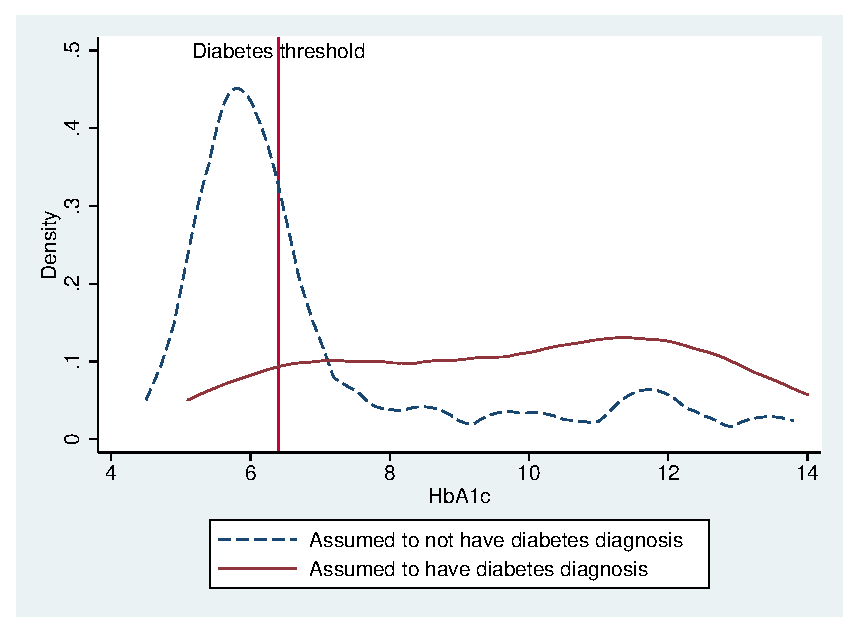
\includegraphics[width=.5\linewidth]{figures/kdensity_hba1c_inconsist.eps}\\
\end{center}
\end{figure}
\DIFaddend 





\end{appendix}

\subsection*{Acknowledgements}

We are grateful to the participants at the European Health Economics Association PhD-Supervisor conference September 2015 in Paris, the Health, Education and Labor Market Outcomes Workshop at the WifOR Institute in October 2015 in Darmstadt, Germany, seminar participants at the Centre for Health Economics at York University, and Max Bachmann for helpful comments.




%\noindent \bibliographystyle{elsarticle-harv} 

\printbibliography

%\bibliography{/home/till/Dokumente/BibTex/Second_Mexico_paper-Article}
\end{document}

